\chapter{常微分方程}
\label{chap:ordinary-differential-equations}

一间屋子比室外暖和，热量就会不断散出；暖气开着，热量又不断补进来。温度并不是每隔一分钟才跳一次，而是在每个瞬间都以某个速率变化，这个速率又取决于此刻屋里有多热。一只摆也是这样：此刻的角度和角速度决定了下一瞬间往哪边摆、摆多快。这类规律只说出“此刻往哪里走、走多快”，却没有直接给出一小时以后的状态。

于是有一连串自然的问题。只知道每个瞬间的变化率和出发点，整条轨迹是否就确定了，会不会有两条不同的轨迹满足同一规律，又能延续多久？初温量错了一点、暖气功率改了一点，一小时后的温度会差多少？哪些方程能直接写出解，长期来看轨迹趋向哪里，是停在某个平衡、绕着一条闭曲线转，还是越走越远？计算机只能一步一步地推进，算出来的轨迹离真实轨迹有多远，为什么有的问题必须换用隐式格式，为什么模拟行星或分子时又要特别照顾能量和相空间体积？

本章依次回答这些问题。第~\ref{sec:ode-ivp}节先说清楚方程和解的含义：向量场规定瞬时方向，积分把方向累计成轨迹；输入只在时间上可测时，解要放宽到绝对连续曲线。第~\ref{sec:ode-well-posedness}节用同一个积分方程回答存在、唯一、能走多远以及数据改变后轨迹怎样变化，并把解组织成从初态到当前状态的演化映射。第~\ref{sec:ode-analytic-solutions}节在能直接算出解的方程上落实这些概念，矩阵指数与状态转移矩阵给出线性系统的完整解法。第~\ref{sec:ode-stability}节转向长期行为，用谱、线性化和Lyapunov函数判断轨迹是否回到平衡，并研究持续输入留下的状态范围。第~\ref{sec:ode-numerics}节把精确流换成一步一步的数值映射，分析误差怎样产生、传播和控制，以及刚性怎样改变方法的选择。第~\ref{sec:ode-hamiltonian}节研究保守运动的特殊结构，说明为什么保持辛结构的低阶方法在长时间模拟中可以胜过高阶通用方法。

两个例子贯穿全章：室温模型$\dot x=-\lambda x+u$代表耗散、可以直接求解的线性系统，摆代表非线性、有能量结构的系统。第~\ref{chap:discrete-dynamical-systems}章研究一步更新直接给出下一状态的离散系统，本章的许多问题与之平行，但连续时间要先由变化率积分出状态，存在性、稳定区域和数值误差都因此出现新的形式。本章只讨论确定性的方程；输入和噪声带有随机性时的方程留到第~\ref{chap:continuous-time-stochastic-processes}章。所用的微积分、矩阵谱和压缩映射来自前置各卷，引用处先说明所用结论。

% 第8章第1节：初值问题与解（向量场与状态方程；微分形式与积分形式）。

\section{初值问题与解}
\label{sec:ode-ivp}

本节先确定要解的是什么：变化率怎样写成状态方程，高阶方程怎样化成一阶系统，以及一条曲线在什么意义下“满足”方程。存在性和唯一性是下一节的问题；这里只把两件事分开，免得在还不知道解是否存在时就谈论它的性质。

\subsection{向量场与状态方程}
\label{sec:ode-vector-fields}

\paragraph{从变化率到状态方程}
把房间相对室外的温差记作$x(t)$，暖气在时刻$t$送入的加热量记作$u(t)$。温差越大，单位时间散失的热量越多；在最简单的模型里散热率与温差成正比，比例系数$\lambda>0$由墙体和通风决定。于是温差的变化率是补进的热量减去散失的热量：
\begin{equation}
  \dot x(t)=-\lambda x(t)+u(t).
  \label{eq:ode-temperature}
\end{equation}
这里$\dot x$表示对时间的导数。式~\eqref{eq:ode-temperature}没有直接说出$x(t)$等于多少，只说出每个瞬间温差朝哪个方向、以多快的速率变化。本章常取$\lambda=0.2$（时间单位为分钟）和恒定加热量$u=0.4$，这时温差为$2$的状态恰好收支平衡：$-0.2\times2+0.4=0$。

摆给出第二种情形。设摆长为$\ell$，摆角为$\theta$，重力加速度为$g$，空气阻力与角速度成正比，系数为$c\geq0$。牛顿第二定律给出$\ddot\theta=-(g/\ell)\sin\theta-c\dot\theta$。为简化记号，选时间单位使$g/\ell=1$。这个方程含有二阶导数：只知道此刻的角度，还不能决定下一瞬间的变化，因为同一个角度上摆可能正向左摆，也可能正向右摆。

两种情形可以写进同一个框架。把此刻需要知道的量排成状态向量$\bm x(t)\in\mathbb R^d$，把给定的外部作用写成输入$\bm u(t)\in\mathbb R^m$，变化规律写成函数$\bm f$：
\begin{equation}
  \dot{\bm x}(t)=\bm f\bigl(t,\bm x(t),\bm u(t)\bigr),\qquad \bm x(t_0)=\bm x_0.
  \label{eq:ode-ivp-input}
\end{equation}
第一式是状态方程，第二式指定出发的时刻和状态。完整的问题还要说清三样东西：时间在哪个区间$I\ni t_0$中取值；状态允许在哪个开集$D\subseteq\mathbb R^d$中取值，例如浓度只能为正、摆的状态可以取遍$\mathbb R^2$；输入是哪一条事先给定的函数$\bm u:I\to\mathbb R^m$。

本章总把输入当作已经选定的一条时间函数。代入后得到只依赖时间与状态的函数
\[
  \bm g(t,\bm x)=\bm f\bigl(t,\bm x,\bm u(t)\bigr),
\]
状态方程就成为$\dot{\bm x}=\bm g(t,\bm x)$。根据当前状态选择输入，是控制问题要做的事；那时输入本身依赖状态，代入后仍得到一个$\bm g$，但它的性质取决于所选的反馈规则。把“选哪条输入”与“给定输入后怎样求解”分开，本章的结论才能在控制问题中直接使用。

\begin{definition}[初值问题]
  \label{def:ode-ivp}
  设$I\subseteq\mathbb R$是区间，$D\subseteq\mathbb R^d$是开集，$\bm g:I\times D\to\mathbb R^d$，$t_0\in I$，$\bm x_0\in D$。\term{初值问题}（initial value problem）是寻找区间$J\subseteq I$（$t_0\in J$）上的曲线$\bm x:J\to D$，使
  \begin{equation}
    \dot{\bm x}(t)=\bm g\bigl(t,\bm x(t)\bigr),\qquad \bm x(t_0)=\bm x_0.
    \label{eq:ode-ivp}
  \end{equation}
  $\bm g$称为方程的\term{向量场}。“曲线满足方程”的确切含义由定义~\ref{def:ode-classical-solution}和定义~\ref{def:ode-caratheodory-solution}给出。
\end{definition}

方程中只出现状态的一阶导数，因此称为\term{常微分方程}（ordinary differential equation, ODE）；“常”指未知函数只依赖一个自变量$t$。未知量若是依赖时间和空间位置的场，导数就会对多个变量求，得到第~\ref{chap:partial-differential-equations}章的偏微分方程。

\paragraph{斜率场与积分曲线}
在纸上画出向量场，比读公式更容易看出解的样子。对温度模型，在$(t,x)$平面的每个格点上画一小段线段，斜率等于$-0.2x+0.4$。图~\ref{fig:ode-slope-field}(a)显示：温差高于$2$的地方线段向下倾斜，低于$2$的地方向上倾斜，正好在$x=2$处变平。解就是一条处处与这些线段相切的曲线；从不同高度出发的曲线都被线段“引导”向$x=2$靠拢，越靠近越平缓。

\begin{figure*}[htbp]
  \centering
  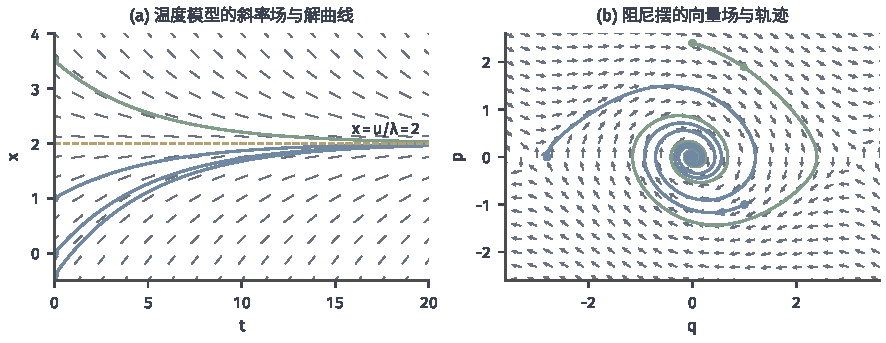
\includegraphics[width=150mm]{figures/03-optimization-evolution-and-signals/02-processes-and-trajectory-evolution/matplotlib/ode-slope-field/figure.pdf}
  \caption{向量场与解曲线。(a)温度模型$\dot x=-0.2x+0.4$的斜率场：每条灰色短线的斜率等于该点的变化率；蓝、绿曲线是从$x_0=-0.4,0,1,3.5$出发的解$x(t)=2+(x_0-2)e^{-0.2t}$，黄色虚线是收支平衡的温差$2$。(b)阻尼摆$\dot q=p$，$\dot p=-\sin q-0.3p$的相平面：箭头只表示向量场方向（已归一化长度），三条轨迹分别从$(-2.8,0)$、$(0,2.4)$、$(1,-1)$出发，计算到$t=25$。}
  \label{fig:ode-slope-field}
\end{figure*}

摆的状态是二维的，可以换一种画法。把角度$q=\theta$和角速度$p=\dot\theta$作为平面坐标，在每一点画出向量$\bigl(p,-\sin q-cp\bigr)$。这个平面称为\term{相平面}，更一般的状态空间也称\term{相空间}（phase space）。图~\ref{fig:ode-slope-field}(b)中，轨迹顺着箭头前进：上半平面$p>0$时角度增大，箭头向右；摆角为正时重力把角速度往下拉，箭头向下。阻尼使每一圈都比上一圈小，轨迹螺旋地落向原点。这里的时间不再是一条坐标轴，而是隐含在沿曲线前进的快慢中；这种画法要求向量场不显含时间，下面马上说明这一点。

\paragraph{高阶方程化为一阶系统}
摆的二阶方程化成了两个一阶方程
\[
  \dot q=p,\qquad \dot p=-\sin q-cp.
\]
做法是把“预测未来需要知道的量”全部放进状态。一般地，若标量未知函数$y$满足$n$阶方程
\[
  y^{(n)}=h\bigl(t,y,\dot y,\ldots,y^{(n-1)}\bigr),
\]
令$x_1=y$，$x_2=\dot y$，……，$x_n=y^{(n-1)}$，就得到一阶系统
\[
  \dot x_1=x_2,\quad\ldots,\quad\dot x_{n-1}=x_n,\quad\dot x_n=h(t,x_1,\ldots,x_n).
\]
相应地，初值必须同时给出$y(t_0),\dot y(t_0),\ldots,y^{(n-1)}(t_0)$这$n$个数。这与第~\ref{chap:discrete-dynamical-systems}章选择离散状态的原则相同：状态要足以决定未来的变化。高阶标量方程与一阶向量系统描述的是同一个对象，只是记号不同；本章的一般理论都对一阶系统陈述。

\paragraph{自治与非自治、线性与非线性}
两组分类经常被混在一起，需要分别说明。若向量场不显含时间，即$\bm g(t,\bm x)=\bm g(\bm x)$，称方程为\term{自治}的（autonomous），否则为非自治的。摆是自治的；温度模型在加热量随时间变化时是非自治的，即使散热系数恒定。自治方程的一个好处正是上面的相平面：同一状态上的方向永远相同，所以可以把方向箭头画在状态空间里而不必记录时间。非自治方程总能通过把时间当作一个新坐标$x_{d+1}=t$、$\dot x_{d+1}=1$改写成自治形式，代价是维数加一。

若$\bm g(t,\bm x)=\bm A(t)\bm x+\bm b(t)$，其中$\bm A(t)\in\mathbb R^{d\times d}$与$\bm b(t)\in\mathbb R^d$只依赖时间，称方程为线性的；$\bm b$不为零时它关于状态其实是仿射的，习惯上仍叫线性方程，$\bm b$称为强迫项。温度模型是线性的，摆因为含$\sin q$而是非线性的。线性与否、自治与否是两项独立的性质：常系数线性系统配上时变输入是线性非自治的，摆是非线性自治的。

\paragraph{与离散更新的对照}
第~\ref{chap:discrete-dynamical-systems}章的一步更新$\bm x_{n+1}=\bm F(\bm x_n)$直接给出下一状态；向量场只给出此刻的瞬时方向。要得到有限时间后的状态，必须沿途把方向累计起来。若在一小段时间$h$内把变化率冻结为起点的值，就得到近似
\[
  \bm x(t+h)\approx\bm x(t)+h\,\bm g\bigl(t,\bm x(t)\bigr).
\]
对温度模型取$h=1$，这个近似是$x(t+1)\approx0.8\,x(t)+u$；而后文第~\ref{sec:ode-constant-linear}小节会算出，在加热量保持不变时，精确的一分钟转移系数是$e^{-0.2}\approx0.8187$。两者接近但不相同，差别来自一分钟之内温差也在变，散热率也随之变化。离散更新与连续方程之间的这种关系，在第~\ref{sec:ode-numerics}节系统讨论。

\subsection{微分形式与积分形式}
\label{sec:ode-integral-form}

\paragraph{经典解与积分方程}
最直接的解的概念是逐点满足方程的可微曲线。

\begin{definition}[经典解]
  \label{def:ode-classical-solution}
  设$\bm g$在$I\times D$上连续。区间$J\ni t_0$上的曲线$\bm x:J\to D$若连续可微，满足$\bm x(t_0)=\bm x_0$，并且$\dot{\bm x}(t)=\bm g(t,\bm x(t))$对每个$t\in J$成立，称为初值问题~\eqref{eq:ode-ivp}的\term{经典解}（classical solution）。
\end{definition}

把方程两边从$t_0$积分到$t$，导数就被换成了状态的增量。这样得到的积分方程不再出现导数，是下一节证明存在唯一性的出发点。

\begin{lemma}[经典解的积分刻画]
  \label{lem:ode-integral-equation}
  设$\bm g$在$I\times D$上连续，$\bm x:J\to D$连续。则$\bm x$是初值问题~\eqref{eq:ode-ivp}的经典解，当且仅当
  \begin{equation}
    \bm x(t)=\bm x_0+\int_{t_0}^t\bm g\bigl(s,\bm x(s)\bigr)\,\mathrm ds\qquad\text{对每个}t\in J.
    \label{eq:ode-integral-equation}
  \end{equation}
\end{lemma}

\begin{proof}
  若$\bm x$是经典解，则$\dot{\bm x}$连续，微积分基本定理给出$\bm x(t)-\bm x(t_0)=\int_{t_0}^t\dot{\bm x}(s)\,\mathrm ds$，再代入方程与初值即得式~\eqref{eq:ode-integral-equation}。反过来，若$\bm x$连续并满足式~\eqref{eq:ode-integral-equation}，则被积函数$s\mapsto\bm g(s,\bm x(s))$是连续函数的复合，因而连续；微积分基本定理说明右端关于$t$连续可微，导数等于$\bm g(t,\bm x(t))$。于是$\bm x$连续可微并满足方程，代入$t=t_0$得到初值。
\end{proof}

式~\eqref{eq:ode-integral-equation}有一个直观的读法：此刻的状态等于出发时的状态，加上一路上速度的累计。对标量方程，它就是“初值加上速度曲线下的面积”。这个读法把求解问题变成了一个自洽条件：曲线$\bm x$决定了沿途的速度$\bm g(s,\bm x(s))$，速度的累计又必须重新给出同一条曲线。

\paragraph{只可测的输入}
经典解要求$\bm g$关于时间连续，实际的输入却常常有跳变。设暖气在前$5$分钟以$u=0.4$加热，随后关闭，即
\[
  u(t)=\begin{cases}0.4,&0\leq t<5,\\0,&t\geq5.\end{cases}
\]
在$t=5$处方程右端跳变，任何可微曲线都无法在这一点同时满足左右两侧的方程。但积分方程~\eqref{eq:ode-integral-equation}对这种分段常值输入仍然有意义，而且房间的温度在物理上确实随时间连续变化。

\begin{example}[开关暖气下的温差]
  \label{ex:ode-switched-heating}
  取$\lambda=0.2$，$x(0)=0$，输入如上。在$[0,5]$上，$x(t)=2(1-e^{-0.2t})$，于是$x(5)=2(1-e^{-1})\approx1.2642$。$t\geq5$时只剩散热，从这个值出发得到$x(t)=1.2642\,e^{-0.2(t-5)}$。两段在$t=5$处连在一起，但左导数$-0.2\times1.2642+0.4\approx0.1472$与右导数$-0.2\times1.2642\approx-0.2528$不同，曲线在这里出现折角。直接验算可知，这条曲线对每个$t\geq0$都满足积分方程~\eqref{eq:ode-integral-equation}，并且除$t=5$外处处满足微分方程。
\end{example}

这个例子提示应当放宽解的概念：允许在一个“可以忽略”的时刻集合上不可导，只要积分关系成立。可是放宽到什么程度？仅要求曲线连续、几乎处处满足方程是不够的。Cantor函数$c:[0,1]\to[0,1]$连续、单调不减，在Cantor集之外导数为零，而Cantor集的Lebesgue测度为零；可它从$c(0)=0$升到$c(1)=1$，并不是常数。若只要求几乎处处满足方程，Cantor函数就会成为方程$\dot x=0$、$x(0)=0$的一个“解”，零解的唯一性也就无从谈起。问题在于Cantor函数的全部变化都藏在导数看不见的零测集上，不能由导数积分还原。

能够由导数积分还原的函数恰好是绝对连续函数：若$x$在$[a,b]$上绝对连续，则它几乎处处可导，导数可积，并且$x(t)=x(a)+\int_a^t\dot x(s)\,\mathrm ds$；反之，可积函数的不定积分总是绝对连续的。这一刻画及Cantor函数为什么不绝对连续，可参考\BookChapterRef{chap:integration}{卷二“积分”章}。向量值曲线按分量理解，于是得到下面的定义。

\begin{definition}[绝对连续曲线]
  \label{def:ode-absolutely-continuous-curve}
  有限闭区间$[a,b]$上的曲线$\bm x:[a,b]\to\mathbb R^d$称为\term{绝对连续曲线}，若存在可积函数$\bm v\in L^1([a,b];\mathbb R^d)$，使$\bm x(t)=\bm x(a)+\int_a^t\bm v(s)\,\mathrm ds$对每个$t\in[a,b]$成立。此时$\dot{\bm x}=\bm v$几乎处处成立。一般区间上的曲线若在其中每个有限闭子区间上绝对连续，称为局部绝对连续。
\end{definition}

为让积分方程中的被积函数可积，需要对$\bm g$加下面三条要求，它们合称为\term{Carathéodory条件}：
\begin{enumerate}
  \item 对每个固定的$\bm x\in D$，$t\mapsto\bm g(t,\bm x)$可测；
  \item 对几乎每个$t\in I$，$\bm x\mapsto\bm g(t,\bm x)$连续；
  \item 对每个紧集$K\subseteq D$，存在在$I$的每个有限闭子区间上可积的函数$m_K\geq0$，使$\|\bm g(t,\bm x)\|_2\leq m_K(t)$对几乎每个$t$与全部$\bm x\in K$成立。
\end{enumerate}
前两条保证对每条连续曲线$\bm x$，复合函数$s\mapsto\bm g(s,\bm x(s))$可测；第三条保证当曲线留在紧集$K$中时，这个复合函数可积。若$\bm f$关于$(t,\bm x,\bm u)$连续，输入$\bm u$可测且局部有界，则$\bm g(t,\bm x)=\bm f(t,\bm x,\bm u(t))$满足这三条：第三条中的上界可取为$\bm f$在一个紧集上的最大值。开关暖气的例子正是这种情形。

\begin{definition}[Carathéodory解]
  \label{def:ode-caratheodory-solution}
  设$\bm g$满足Carathéodory条件。区间$J\ni t_0$上局部绝对连续的曲线$\bm x:J\to D$，若对每个$t\in J$满足积分方程~\eqref{eq:ode-integral-equation}，称为初值问题的\term{Carathéodory解}。等价地，$\bm x(t_0)=\bm x_0$且$\dot{\bm x}(t)=\bm g(t,\bm x(t))$对几乎每个$t\in J$成立。
\end{definition}

两种表述等价，正是绝对连续曲线的作用：积分方程给出的曲线自动绝对连续并几乎处处满足方程；反过来，一条几乎处处满足方程的绝对连续曲线可以由导数积分还原，因而满足积分方程。当$\bm g$连续时，引理~\ref{lem:ode-integral-equation}说明Carathéodory解就是经典解，所以这是对经典概念的推广而不是替换。本章在$\bm g$连续时直接说“解”指经典解；输入只可测时说“解”指Carathéodory解。

\paragraph{满足方程与解的存在是两个问题}
到这里只回答了“什么样的曲线算解”，还没有回答“这样的曲线是否存在、有几条、能延续多久”。积分方程~\eqref{eq:ode-integral-equation}把后一组问题变成了一个不动点问题：在曲线组成的集合上，映射
\[
  \bm x\longmapsto\bm x_0+\int_{t_0}^{\cdot}\bm g\bigl(s,\bm x(s)\bigr)\,\mathrm ds
\]
把一条候选曲线送到另一条曲线，解就是被送回自身的曲线。下一节研究这个映射在什么条件下恰有一个不动点。

% 第8章第2节：存在、唯一与连续依赖（局部存在唯一；最大解与爆炸；连续依赖与变分方程；演化映射与流）。

\section{存在、唯一与连续依赖}
\label{sec:ode-well-posedness}

本节始终围绕积分方程~\eqref{eq:ode-integral-equation}展开，但依次回答三个不同的问题。第一，在出发点附近，积分映射是否恰有一个不动点？第二，局部解能延续多久，延续不下去时发生了什么？第三，初值、输入或向量场改变一点，轨迹会改变多少？三个问题使用的条件不同：局部问题只需要向量场在出发点附近的性质，延续问题需要增长控制，比较问题需要沿两条轨迹共同成立的Lipschitz常数。最后把这些结论组织成从初态到当前状态的演化映射。

\subsection{局部存在与唯一性}
\label{sec:ode-local-existence}

\paragraph{Picard迭代：把猜测反复代入积分}
积分方程把解描述成一个自洽条件。一个朴素的求解办法是：先随便猜一条曲线，算出沿它的速度并积分，得到一条新曲线；再把新曲线当作猜测，重复这个过程。记积分映射为
\begin{equation}
  (\mathcal T\bm z)(t)=\bm x_0+\int_{t_0}^t\bm g\bigl(s,\bm z(s)\bigr)\,\mathrm ds,
  \label{eq:ode-picard-map}
\end{equation}
从常值曲线$\bm x^{(0)}(t)\equiv\bm x_0$出发，令$\bm x^{(k+1)}=\mathcal T\bm x^{(k)}$，这一列曲线称为\term{Picard迭代}（Picard iteration）。

\begin{example}[指数函数的Picard迭代]
  \label{ex:ode-picard-exponential}
  取$\dot x=x$，$x(0)=1$。从$x^{(0)}\equiv1$出发，
  \[
    x^{(1)}(t)=1+\int_0^t1\,\mathrm ds=1+t,\qquad
    x^{(2)}(t)=1+\int_0^t(1+s)\,\mathrm ds=1+t+\frac{t^2}{2},
  \]
  归纳可得$x^{(k)}(t)=\sum_{j=0}^kt^j/j!$，恰是$e^t$的Taylor多项式。由Taylor余项，$0\leq e^t-x^{(k)}(t)\leq t^{k+1}e^t/(k+1)!$对$t\geq0$成立。在$t=2$处，$x^{(4)}(2)=7$，而$e^2\approx7.389$。
\end{example}

图~\ref{fig:ode-picard}(b)画出前几次迭代。每次迭代都在离出发点更远的一段时间上贴近真解：$x^{(1)}$只在$t=0$附近与$e^t$相切，$x^{(4)}$已在$[0,1]$上几乎重合。迭代从出发点向外“修正”曲线，因为积分从$t_0$开始累计，越远的时刻累计的误差越多，也需要越多次迭代才能消除。

\begin{figure*}[htbp]
  \centering
  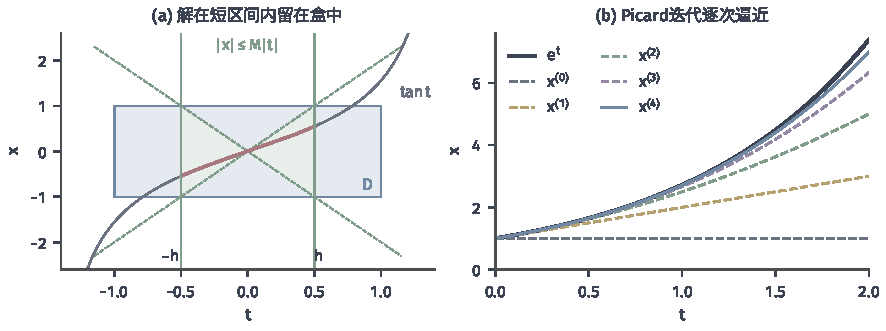
\includegraphics[width=150mm]{figures/03-optimization-evolution-and-signals/02-processes-and-trajectory-evolution/matplotlib/ode-picard/figure.pdf}
  \caption{局部存在性的两个画面。(a)方程$\dot x=1+x^2$，$x(0)=0$：蓝色矩形是$D=[-1,1]\times[-1,1]$，其中$|\dot x|\leq M=2$；绿色虚线是斜率$\pm M$的锥面，任何解在离开矩形之前都被限制在锥内。取$h=\min(a,b/M)=0.5$，红色的真解$\tan t$在$|t|\leq h$上留在矩形中；灰色是$\tan t$在更大区间上的部分。(b)方程$\dot x=x$，$x(0)=1$的Picard迭代$x^{(0)},\ldots,x^{(4)}$（虚线到实线）与真解$e^t$（黑色粗线）。}
  \label{fig:ode-picard}
\end{figure*}

迭代是否总能收敛，收敛的极限是否唯一？关键在于映射$\mathcal T$是否在某个完备的曲线空间里把两条曲线的距离缩小。设$\bm g$关于状态满足Lipschitz条件，常数为$L$，即$\|\bm g(t,\bm x)-\bm g(t,\bm y)\|_2\leq L\|\bm x-\bm y\|_2$。对两条曲线$\bm z_1,\bm z_2$，
\[
  \begin{aligned}
  \bigl\|(\mathcal T\bm z_1)(t)-(\mathcal T\bm z_2)(t)\bigr\|_2
  &\leq\left|\int_{t_0}^tL\|\bm z_1(s)-\bm z_2(s)\|_2\,\mathrm ds\right|\\
  &\leq L|t-t_0|\,\sup_s\|\bm z_1(s)-\bm z_2(s)\|_2.
  \end{aligned}
\]
时间区间长度不超过$h$时，$\mathcal T$至少把一致距离缩小到原来的$Lh$倍；$Lh<1$便是压缩。完备度量空间上的压缩映射恰有一个不动点，并且从任意初始点出发的迭代都收敛到它，这就是压缩映射定理，可参考\BookChapterRef{chap:metric-spaces}{卷二“度量空间”章}。剩下的问题是让$\mathcal T$把一个完备集合映回自身。

\paragraph{在短时间的曲线空间里压缩}
向量场通常只在出发点附近有界、有Lipschitz常数，所以只能在一个盒子里工作。图~\ref{fig:ode-picard}(a)画出这个盒子：时间方向半宽$a$，状态方向半径$b$。若盒中$\|\bm g\|_2\leq M$，任何解在离开盒子之前，状态偏离$\bm x_0$的距离不超过$M|t-t_0|$，即被限制在斜率为$\pm M$的锥里。只要时间不超过$b/M$，锥就还在盒子之内，解没有机会离开。于是时间区间要同时满足两个限制：留在盒中需要$Mh\leq b$，压缩需要$Lh<1$。

为此先说明关于状态的局部条件。称$\bm g$在$I\times D$上关于状态\term{局部Lipschitz}，若每一点$(t,\bm x)$都有邻域$U$与常数$L_U$，使$U$中同一时刻的两点满足$\|\bm g(t,\bm y)-\bm g(t,\bm z)\|_2\leq L_U\|\bm y-\bm z\|_2$。若$\bm g$对状态有连续偏导数，它就是局部Lipschitz的：在以$\bm x$为心的闭球上，Jacobian矩阵的范数有界，中值不等式沿两点间的线段给出Lipschitz常数。摆的向量场$(p,-\sin q-cp)$以及一切多项式向量场都属于这种情形。

\begin{theorem}[局部存在唯一性]
  \label{thm:ode-picard-lindelof}
  设$a,b>0$，$R=[t_0-a,t_0+a]\times\{\bm x:\|\bm x-\bm x_0\|_2\leq b\}\subseteq I\times D$，$\bm g$在$R$上连续，并且存在$L\geq0$使$R$中同一时刻的两点满足$\|\bm g(t,\bm y)-\bm g(t,\bm z)\|_2\leq L\|\bm y-\bm z\|_2$。记$M=\max_R\|\bm g\|_2$，取$h>0$满足
  \[
    h\leq a,\qquad Mh\leq b,\qquad Lh<1.
  \]
  则在$J=[t_0-h,t_0+h]$上初值问题~\eqref{eq:ode-ivp}恰有一个解；并且对任何包含$t_0$的区间$J'\subseteq J$，$J'$上的解都等于这个解在$J'$上的限制。
\end{theorem}

\begin{proof}
  令$\mathcal X$为$J$上满足$\|\bm z(t)-\bm x_0\|_2\leq b$（对每个$t\in J$）的连续曲线全体，取一致距离$\|\bm z_1-\bm z_2\|_\infty=\max_{t\in J}\|\bm z_1(t)-\bm z_2(t)\|_2$。$J$上的连续曲线在一致距离下构成完备空间，$\mathcal X$是其中的闭子集，因而也完备。

  \emph{映回。}对$\bm z\in\mathcal X$，点$(s,\bm z(s))$都在$R$中，所以式~\eqref{eq:ode-picard-map}的被积函数连续且范数不超过$M$。于是$\mathcal T\bm z$连续，并且$\|(\mathcal T\bm z)(t)-\bm x_0\|_2\leq M|t-t_0|\leq Mh\leq b$，即$\mathcal T\bm z\in\mathcal X$。

  \emph{压缩。}对$\bm z_1,\bm z_2\in\mathcal X$，上一段之前的估计给出$\|\mathcal T\bm z_1-\mathcal T\bm z_2\|_\infty\leq Lh\|\bm z_1-\bm z_2\|_\infty$，而$Lh<1$。由压缩映射定理，$\mathcal T$在$\mathcal X$中恰有一个不动点$\bm x$，由引理~\ref{lem:ode-integral-equation}它是$J$上的解。

  \emph{任何解都在盒中。}设$\bm y$是$J'$上的解，只看$t\geq t_0$的一侧，另一侧对称。令$t^\ast$为使$\bm y$在$[t_0,t^\ast]$上留在闭球中的最大时刻（闭球与$\bm y$的连续性保证最大值取到）。若$t^\ast<\sup J'$，则在$[t_0,t^\ast]$上点$(s,\bm y(s))$都在$R$中，积分方程给出$\|\bm y(t^\ast)-\bm x_0\|_2\leq M(t^\ast-t_0)<Mh\leq b$。严格不等式与连续性说明$\bm y$在$t^\ast$之后的一小段时间仍在球内，与$t^\ast$的最大性矛盾。因此$\bm y$在整个$J'$上留在球中。

  \emph{唯一。}把$\mathcal X$与$\mathcal T$中的$J$换成$J'$，上述映回与压缩的论证不变，所以$J'$上的不动点唯一。$\bm y$与$\bm x$在$J'$上的限制都是这个不动点，故二者相等。
\end{proof}

条件$Lh<1$只是为了让一致距离直接收缩，并不是本质限制。换用加权距离$\|\bm z\|_{L}=\max_{t\in J}e^{-2L|t-t_0|}\|\bm z(t)\|_2$，同样的估计给出
\[
  \bigl\|(\mathcal T\bm z_1-\mathcal T\bm z_2)(t)\bigr\|_2
  \leq L\left|\int_{t_0}^te^{2L|s-t_0|}\,\mathrm ds\right|\,\|\bm z_1-\bm z_2\|_{L}
  \leq\frac12e^{2L|t-t_0|}\|\bm z_1-\bm z_2\|_{L},
\]
即$\mathcal T$在加权距离下总以因子$\tfrac12$压缩，不论$h$多大。所以局部解的存在时间只受$h\leq a$与$Mh\leq b$限制，也就是只受“解不能跑出盒子”的限制。图~\ref{fig:ode-picard}(a)中的方程$\dot x=1+x^2$取$a=b=1$，得$M=2$，$h=0.5$；真解$\tan t$在$|t|\leq0.5$上满足$|\tan t|\leq0.547<1$，确实留在盒内，而它在$t=\pi/2$处趋于无穷，说明局部结论不能随意扩大到长时间区间。

把连续性换成Carathéodory条件，同一证明几乎原样适用，只是把常数换成可积函数。

\begin{theorem}[可测输入下的局部存在唯一性]
  \label{thm:ode-caratheodory-local}
  设$\bm g$满足第~\ref{sec:ode-integral-form}小节的Carathéodory条件，并且对每个紧集$K\subseteq D$存在在$I$的有限闭子区间上可积的函数$\ell_K\geq0$，使$\|\bm g(t,\bm y)-\bm g(t,\bm z)\|_2\leq\ell_K(t)\|\bm y-\bm z\|_2$对几乎每个$t$与全部$\bm y,\bm z\in K$成立。则存在$h>0$，使初值问题在$[t_0-h,t_0+h]\cap I$上恰有一个Carathéodory解。
\end{theorem}

\begin{proof}
  取闭球$K=\{\bm x:\|\bm x-\bm x_0\|_2\leq b\}\subseteq D$及其上的$m_K,\ell_K$。由积分的绝对连续性，可取$h>0$使$\int_{t_0-h}^{t_0+h}m_K\leq b$且$\int_{t_0-h}^{t_0+h}\ell_K<1$。在定理~\ref{thm:ode-picard-lindelof}的证明中，用$\int m_K$代替$Mh$，用$\int\ell_K$代替$Lh$，映回、压缩与“任何解都在盒中”三步的不等式都照样成立；不动点由积分给出，因而绝对连续。
\end{proof}

开关暖气的例子满足这两个定理之一吗？温度模型的向量场$-0.2x+u(t)$对状态是全局Lipschitz的，常数$0.2$，而$u$分段常值、可测有界，所以定理~\ref{thm:ode-caratheodory-local}适用，示例~\ref{ex:ode-switched-heating}中的折线状曲线就是唯一的Carathéodory解。

\paragraph{只有连续性时：等待后离开}
Lipschitz条件不能简单删去。考虑
\[
  \dot x=\sqrt{|x|},\qquad x(0)=0.
\]
零函数满足方程与初值，是一个解。对任意$c\geq0$，曲线
\[
  x_c(t)=\begin{cases}0,&0\leq t\leq c,\\(t-c)^2/4,&t>c\end{cases}
\]
也是解：在$t>c$处$\dot x_c=(t-c)/2=\sqrt{x_c}$，在$t=c$处左右导数都是零。于是同一个初值有无穷多个解，它们在原点“等待”任意长时间后离开，如图~\ref{fig:ode-nonunique}所示。

\begin{figure}[htbp]
  \centering
  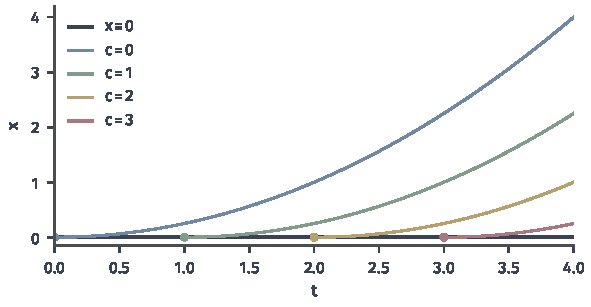
\includegraphics[width=100mm]{figures/03-optimization-evolution-and-signals/02-processes-and-trajectory-evolution/matplotlib/ode-nonunique/figure.pdf}
  \caption{方程$\dot x=\sqrt{|x|}$、$x(0)=0$的一族解。黑线是零解；彩色曲线是$x_c(t)=(t-c)^2/4$（$t>c$），在$c=0,1,2,3$之前停在原点（圆点标出离开时刻）。向量场连续，但在$x=0$处不满足Lipschitz条件。}
  \label{fig:ode-nonunique}
\end{figure}

问题出在原点附近。$\sqrt{|x|}/|x|=1/\sqrt{|x|}$在$x\to0$时无界，所以不存在包含原点的Lipschitz邻域。直观地说，向量场在原点为零，却在原点旁边以$\sqrt{|x|}$的速度推开状态；这个推力随距离缩小得太慢，使得从原点离开只需要有限时间。第~\ref{sec:ode-separable-linear}小节会用“时间等于路程除以速度的积分”把这个现象说得更清楚。若初值$x(0)=1$，则解在一段时间内远离原点，那里$\sqrt{x}$可微，定理~\ref{thm:ode-picard-lindelof}照样给出局部唯一性。

只要求连续时，存在性仍然成立：若$\bm g$在$(t_0,\bm x_0)$的邻域内连续，则初值问题至少有一个局部解。这就是Peano定理。证明的思路是用越来越细的Euler折线逼近解，这些折线在盒中有共同的斜率界$M$，因而一致有界、等度连续，由Arzelà--Ascoli定理可抽出一致收敛的子列，其极限满足积分方程\scite{math-hairer1993ode}。Peano定理只保证存在，正如上例所示，不保证唯一。本章后文的结论都建立在局部Lipschitz条件之上，Peano定理只作补充。

\subsection{最大解、延拓与爆炸}
\label{sec:ode-maximal-solutions}

本小节假设时间区间$I$是开区间，$\bm g$在$I\times D$上连续并关于状态局部Lipschitz。定理~\ref{thm:ode-picard-lindelof}在每个出发点附近给出局部解；现在问这些局部解能拼接成多长的一条。

\paragraph{用唯一性拼接局部解}
设$\bm x$定义在区间$J_1$上，$\bm y$定义在区间$J_2$上，二者都是同一初值问题的解。它们在公共区间$J_1\cap J_2$上必须相同。令$S=\{t\in J_1\cap J_2:\bm x(t)=\bm y(t)\}$。$S$包含$t_0$，并且由连续性在$J_1\cap J_2$中是闭集。$S$也是开集：若$\bm x(t_1)=\bm y(t_1)$，则$\bm x$与$\bm y$都是从$(t_1,\bm x(t_1))$出发的解，定理~\ref{thm:ode-picard-lindelof}说明它们在$t_1$附近的一个区间上相同。区间是连通的，既开又闭的非空子集只能是整个区间，所以$S=J_1\cap J_2$。

于是所有解可以无矛盾地拼在一起：把每个解的定义区间并起来，在并集的每一点上取任意一个在该点有定义的解的值。这样得到的曲线仍是解，而且任何解都是它的限制。

\begin{definition}[最大解]
  \label{def:ode-maximal-solution}
  初值问题的解$\bm x:J\to D$若不能延拓为更大区间上的解，称为\term{最大解}（maximal solution），$J$称为\term{最大存在区间}，记为$(\omega_-,\omega_+)$。
\end{definition}

最大存在区间是开区间：若它包含右端点$\omega_+<\sup I$，从$(\omega_+,\bm x(\omega_+))$出发的局部解就能把它再延长一段。若$\omega_+=\sup I$，解在整个未来都有定义，称为正向全局存在；若$(\omega_-,\omega_+)=I$，称为\term{全局解}。

\paragraph{有限时间爆炸}
光滑的向量场也可能只有有限的$\omega_+$。考虑
\[
  \dot x=x^2,\qquad x(0)=x_0>0.
\]
直接验算可知$x(t)=x_0/(1-x_0t)$是解，它在$t\uparrow1/x_0$时趋于无穷，所以$\omega_+=1/x_0$。初值越大，爆炸越早，见图~\ref{fig:ode-blowup}(a)。

\begin{figure*}[htbp]
  \centering
  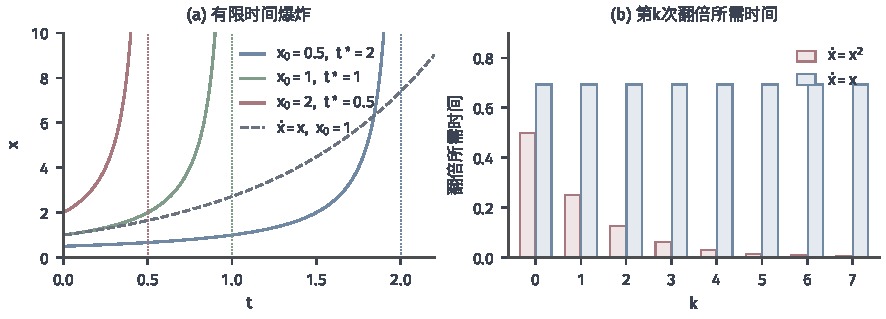
\includegraphics[width=150mm]{figures/03-optimization-evolution-and-signals/02-processes-and-trajectory-evolution/matplotlib/ode-blowup/figure.pdf}
  \caption{有限时间爆炸。(a)$\dot x=x^2$从$x_0=0.5,1,2$出发的解$x_0/(1-x_0t)$，点线标出爆炸时刻$t^\ast=1/x_0$；灰色虚线是$\dot x=x$、$x_0=1$的解$e^t$，对每个有限时刻都有定义。(b)从$x_0=1$出发，状态从$2^k$增长到$2^{k+1}$所需的时间：$\dot x=x^2$需要$1/2^{k+1}$，总和为$1$；$\dot x=x$每次都需要$\log2\approx0.693$，总和发散。}
  \label{fig:ode-blowup}
\end{figure*}

为什么$\dot x=x^2$会爆炸而$\dot x=x$不会？看状态每翻一番要花多少时间。速度为$x^2$时，从$X$走到$2X$所需时间是
\[
  \int_X^{2X}\frac{\mathrm d\xi}{\xi^2}=\frac1{2X},
\]
越往后翻倍越快；从$1$出发，所有翻倍时间之和$\tfrac12+\tfrac14+\cdots=1$有限，所以有限时间内要翻倍无穷多次。速度为$x$时，每次翻倍都需要$\int_X^{2X}\mathrm d\xi/\xi=\log2$，无穷多次翻倍需要无穷长时间。图~\ref{fig:ode-blowup}(b)把这两列时间并排画出。增长自我加速得足够快时，有限时间就能走完无限长的路。

解还可能以另一种方式停下来：没有趋于无穷，而是撞到状态集合的边界。取$D=(0,\infty)$，$\dot x=-1/x$，$x(0)=1$。由$\frac{\mathrm d}{\mathrm dt}x^2=2x\dot x=-2$得$x(t)=\sqrt{1-2t}$，它在$t\uparrow\tfrac12$时趋于$0$，速度$-1/x$却趋于$-\infty$；状态始终有界，但已经抵达$D$的边界，向量场在那里没有定义。两种情形的共同点是：轨迹终将离开$D$中的每个紧集。

\begin{theorem}[有限时间内离开每个紧集]
  \label{thm:ode-escape}
  设$I$为开区间，$\bm g$在$I\times D$上连续并关于状态局部Lipschitz，$\bm x$是最大解，最大存在区间为$(\omega_-,\omega_+)$。若$\omega_+<\sup I$，则对每个紧集$K\subseteq D$，存在$t_K<\omega_+$，使$\bm x(t)\notin K$对全部$t\in(t_K,\omega_+)$成立。特别地，$D=\mathbb R^d$时$\|\bm x(t)\|_2\to\infty$（$t\uparrow\omega_+$）。$\omega_-$一侧有对称的结论。
\end{theorem}

\begin{proof}
  先为$K$中的全部出发点找一个统一的局部存在时间。取$b>0$使$K_b=\{\bm y:\operatorname{dist}(\bm y,K)\leq b\}$仍是$D$中的紧集，取$a>0$使$T'=[t_0-a,\omega_++a]\subseteq I$。$\bm g$在紧集$T'\times K_b$上连续，因而有界，记上界为$M$。$\bm g$在这个紧集上关于状态还有统一的Lipschitz常数$L$：否则存在同一时刻的点对$(t_n,\bm y_n),(t_n,\bm z_n)$使差商超过$n$；由有界性$\|\bm y_n-\bm z_n\|_2\leq2M/n\to0$，抽子列使两列点收敛到同一点，那一点的Lipschitz邻域最终同时包含两列点，与差商超过$n$矛盾。

  于是对任意$s\in[t_0,\omega_+]$与$\bm\xi\in K$，盒子$[s-a,s+a]\times\{\|\bm y-\bm\xi\|_2\leq b\}$都在$T'\times K_b$中，定理~\ref{thm:ode-picard-lindelof}以统一的$h=\min\{a,b/M,1/(2L)\}$给出从$(s,\bm\xi)$出发、定义在$[s,s+h]$上的解。若某个$t_1\in(\omega_+-h,\omega_+)$使$\bm x(t_1)\in K$，从$(t_1,\bm x(t_1))$出发的解至少延续到$t_1+h>\omega_+$；由拼接论证，它与$\bm x$在公共区间上相同，二者合起来是超过$\omega_+$的解，与最大性矛盾。所以可取$t_K=\omega_+-h$。
\end{proof}

这个定理把“解能否延续”变成了“解是否留在某个紧集中”。只要事先知道轨迹在任意有限时间内都不会跑出某个紧集，最大解就延续到整个$I$。下面的Grönwall不等式正是得到这类先验界的工具。

\paragraph{Grönwall不等式}
设一个非负量$u(t)$的增长率不超过它自身的$b(t)$倍，即$\dot u\leq b(t)u$。把它与等号情形$\dot v=b(t)v$对比，后者的解是$v(t)=v(t_0)\exp\int_{t_0}^tb$，可以想见$u$不会超过这条指数包络。实际使用时，$u$常是两条轨迹之差的范数或状态的范数，它未必可微，能写出的只是积分形式的不等式。下面的引理处理积分形式。

\begin{lemma}[Grönwall积分不等式]
  \label{lem:ode-gronwall}
  \label{lem:action-state-gronwall}
  设$u$是$[t_0,T]$上的非负连续函数，$a\geq0$为常数，$b,r$是$[t_0,T]$上的非负可积函数（例如非负连续函数）。若对每个$t\in[t_0,T]$，
  \begin{equation}
    u(t)\leq a+\int_{t_0}^t\bigl(b(s)u(s)+r(s)\bigr)\,\mathrm ds,
    \label{eq:ode-gronwall-hypothesis}
  \end{equation}
  则对每个$t\in[t_0,T]$，
  \begin{equation}
    u(t)\leq a\exp\left(\int_{t_0}^tb(s)\,\mathrm ds\right)+\int_{t_0}^tr(s)\exp\left(\int_s^tb(\tau)\,\mathrm d\tau\right)\mathrm ds.
    \label{eq:ode-gronwall}
  \end{equation}
  特别地，$r=0$时$u(t)\leq a\exp\int_{t_0}^tb$；若进一步$a=0$，则$u\equiv0$。
\end{lemma}

\begin{proof}
  令$E(t)=a+\int_{t_0}^t(bu+r)$为式~\eqref{eq:ode-gronwall-hypothesis}的右端，则$u\leq E$。$E$是可积函数的不定积分，因而绝对连续，并且几乎处处有$\dot E=bu+r\leq bE+r$，这里用到$b\geq0$与$u\leq E$。令$B(t)=\int_{t_0}^tb$，$e^{-B}$也绝对连续，乘积法则几乎处处给出
  \[
    \frac{\mathrm d}{\mathrm dt}\bigl(E(t)e^{-B(t)}\bigr)=(\dot E-bE)e^{-B}\leq r\,e^{-B}.
  \]
  两个绝对连续函数之积仍绝对连续，可以由导数积分还原。从$t_0$积分到$t$，得$E(t)e^{-B(t)}\leq a+\int_{t_0}^tr(s)e^{-B(s)}\,\mathrm ds$。两边乘以$e^{B(t)}$，再用$u\leq E$，即得式~\eqref{eq:ode-gronwall}。
\end{proof}

$a=0$的特殊情形最常用来证明某个量恒为零：若非负连续的$u$满足$u(t)\leq\int_{t_0}^tb(s)u(s)\,\mathrm ds$，就只能$u\equiv0$。例如两条从同一初值出发的解，其差的范数$u$满足$u(t)\leq L\int_{t_0}^tu$，于是两条解相同；这是唯一性的另一种证明，而且不需要把时间区间缩短。

\paragraph{线性增长与全局存在}
$\dot x=x^2$爆炸，是因为速度的增长快于状态的线性函数。若向量场的大小至多随状态线性增长，Grönwall不等式就能阻止有限时间逃逸。

\begin{theorem}[线性增长下的全局存在]
  \label{thm:ode-global-existence}
  设$I$为开区间，$\bm g$在$I\times\mathbb R^d$上连续并关于状态局部Lipschitz，并且存在$I$上的非负连续函数$b,r$，使
  \[
    \|\bm g(t,\bm x)\|_2\leq b(t)\|\bm x\|_2+r(t)\qquad\text{对全部}(t,\bm x)\in I\times\mathbb R^d.
  \]
  则每个初值问题的最大解都在整个$I$上有定义。
\end{theorem}

\begin{proof}
  只证正向，反向相同。设$\omega_+<\sup I$。在$[t_0,\omega_+)$上，积分方程与增长条件给出
  \[
    \|\bm x(t)\|_2\leq\|\bm x_0\|_2+\int_{t_0}^{\omega_+}r+\int_{t_0}^tb(s)\|\bm x(s)\|_2\,\mathrm ds.
  \]
  $b,r$在紧区间$[t_0,\omega_+]$上连续，因而有界。对每个$T<\omega_+$在$[t_0,T]$上应用引理~\ref{lem:ode-gronwall}（取$r=0$，常数$a$为前两项之和），得$\|\bm x(t)\|_2\leq a\exp\int_{t_0}^{\omega_+}b$，右端与$T$无关。于是$\bm x$在$[t_0,\omega_+)$上留在一个闭球中，与定理~\ref{thm:ode-escape}矛盾。
\end{proof}

若$\bm g$关于状态全局Lipschitz，常数为$L$，则$\|\bm g(t,\bm x)\|_2\leq\|\bm g(t,\bm0)\|_2+L\|\bm x\|_2$，增长条件自动成立。摆的向量场$(p,-\sin q-cp)$的Jacobian矩阵为$\begin{bmatrix}0&1\\-\cos q&-c\end{bmatrix}$，其范数有统一上界，所以摆的每条轨迹都对全部时间存在。系数$\bm A(t),\bm b(t)$在$I$上连续的线性方程同样满足增长条件，解在整个$I$上存在。

增长条件只是充分条件。Logistic方程$\dot x=x(1-x)$的右端按$x^2$增长，可是从$x_0\in[0,1]$出发的解永远留在$[0,1]$中：$x\equiv0$和$x\equiv1$都是解，而拼接论证说明两条不同的解不能在同一时刻取同一值，所以一维自治方程的解不能穿过常值解。留在紧集$[0,1]$中的解由定理~\ref{thm:ode-escape}对全部时间存在。对$x_0>1$，正向解单调下降到$1$，也全局存在；反向时刻的解却在有限时间内趋于$+\infty$。状态集合有边界时，也要用同样的方式检查轨迹是否留在域内，例如浓度模型须说明从正值出发的状态不会变为负值。

\subsection{初值、输入与参数的连续依赖}
\label{sec:ode-continuous-dependence}

\paragraph{把差别送进积分方程}
测量初温时有误差，暖气的实际功率与标称值不同，模型中的散热系数也只是估计。若这些小差别会让一小时后的温度完全不同，模型就无法用于预测。下面把三种差别放进同一个估计：两条轨迹分别由$(\bm x_0,\bm u,\bm f)$与$(\widetilde{\bm x}_0,\widetilde{\bm u},\widetilde{\bm f})$产生，在积分方程中逐项相减。

\begin{theorem}[有限时间连续依赖]
  \label{thm:ode-continuous-dependence}
  设$\bm x,\widetilde{\bm x}:[t_0,T]\to D$分别是
  \[
    \dot{\bm x}=\bm f(t,\bm x,\bm u(t)),\ \bm x(t_0)=\bm x_0
    \qquad\text{与}\qquad
    \dot{\widetilde{\bm x}}=\widetilde{\bm f}(t,\widetilde{\bm x},\widetilde{\bm u}(t)),\ \widetilde{\bm x}(t_0)=\widetilde{\bm x}_0
  \]
  的解，并且两条轨迹都留在集合$K\subseteq D$中。设存在常数$L,L_u\geq0$与可积函数$\rho\geq0$，使对$t\in[t_0,T]$、$\bm y,\bm z\in K$以及输入所取的值$\bm v,\bm w$，
  \[
    \begin{aligned}
      \|\bm f(t,\bm y,\bm v)-\bm f(t,\bm z,\bm v)\|_2&\leq L\|\bm y-\bm z\|_2,\\
      \|\bm f(t,\bm y,\bm v)-\bm f(t,\bm y,\bm w)\|_2&\leq L_u\|\bm v-\bm w\|_2,\\
      \|\bm f(t,\bm y,\bm v)-\widetilde{\bm f}(t,\bm y,\bm v)\|_2&\leq\rho(t).
    \end{aligned}
  \]
  则对每个$t\in[t_0,T]$，
  \begin{equation}
    \begin{aligned}
    \|\bm x(t)-\widetilde{\bm x}(t)\|_2
    \leq{}&e^{L(t-t_0)}\|\bm x_0-\widetilde{\bm x}_0\|_2\\
    &+\int_{t_0}^te^{L(t-s)}\bigl(L_u\|\bm u(s)-\widetilde{\bm u}(s)\|_2+\rho(s)\bigr)\,\mathrm ds.
    \end{aligned}
    \label{eq:ode-continuous-dependence}
  \end{equation}
\end{theorem}

\begin{proof}
  两个积分方程相减，把被积函数之差拆成三段：
  \[
    \begin{aligned}
    \bm f(s,\bm x,\bm u)-\widetilde{\bm f}(s,\widetilde{\bm x},\widetilde{\bm u})
    ={}&\bigl[\bm f(s,\bm x,\bm u)-\bm f(s,\widetilde{\bm x},\bm u)\bigr]\\
    &+\bigl[\bm f(s,\widetilde{\bm x},\bm u)-\bm f(s,\widetilde{\bm x},\widetilde{\bm u})\bigr]\\
    &+\bigl[\bm f(s,\widetilde{\bm x},\widetilde{\bm u})-\widetilde{\bm f}(s,\widetilde{\bm x},\widetilde{\bm u})\bigr],
    \end{aligned}
  \]
  其中各量都在时刻$s$取值。三项依次不超过$L\|\bm x(s)-\widetilde{\bm x}(s)\|_2$、$L_u\|\bm u(s)-\widetilde{\bm u}(s)\|_2$与$\rho(s)$。于是$e(t)=\|\bm x(t)-\widetilde{\bm x}(t)\|_2$满足引理~\ref{lem:ode-gronwall}的假设，其中$a=\|\bm x_0-\widetilde{\bm x}_0\|_2$，$b\equiv L$，$r=L_u\|\bm u-\widetilde{\bm u}\|_2+\rho$。代入式~\eqref{eq:ode-gronwall}即得结论。
\end{proof}

式~\eqref{eq:ode-continuous-dependence}的三项对应三种误差来源：初值误差在开始时注入一次，此后最多按$e^{L(t-t_0)}$放大；输入误差和模型误差在每个时刻$s$持续注入，各自经过剩余时间$t-s$的放大后累计起来。三者来源不同，却都经过同一个传播因子。

定理要求两条轨迹都留在共同的集合$K$中，这是把局部条件用于全局比较时必须付出的代价。若向量场只是局部Lipschitz，可以取$K$为名义轨迹周围半径为$b$的闭管道，它是紧集，因而有统一的常数$L$。只要式~\eqref{eq:ode-continuous-dependence}右端在$[t_0,T]$上小于$b$，扰动后的轨迹就不可能离开这个管道：在它第一次触到管道边界之前，估计都成立，而估计说明它离名义轨迹的距离严格小于$b$。所以初值、输入和模型的扰动足够小时，扰动解在整个$[t_0,T]$上存在，并满足同一估计。

\paragraph{轨迹管}
图~\ref{fig:ode-trajectory-tube}把这个估计画成一束轨迹。对无阻尼摆$\dot q=p$，$\dot p=-\sin q$，Jacobian矩阵$\begin{bmatrix}0&1\\-\cos q&0\end{bmatrix}$的谱范数不超过$1$，所以可取$L=1$。从半径$0.05$的小圆上取$24$个初值，整束轨迹在$t\leq8$内的最大偏差被$0.05e^t$控制；$t=8$时这个上界约为$149$，比相平面本身还大。实际偏差小得多：圆心在$(0,1.2)$时，$t=8$的最大偏差只有约$0.11$。

\begin{figure*}[htbp]
  \centering
  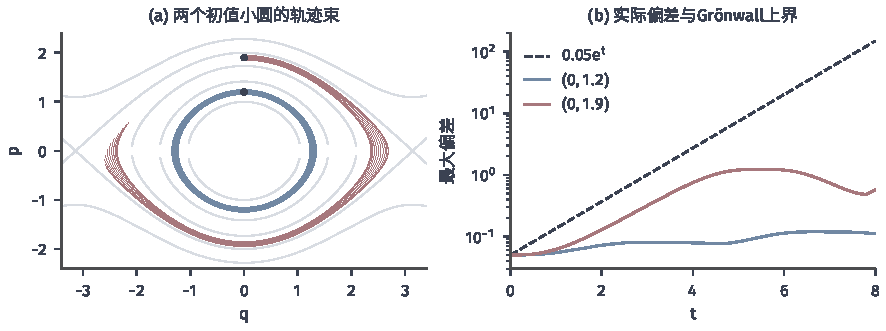
\includegraphics[width=150mm]{figures/03-optimization-evolution-and-signals/02-processes-and-trajectory-evolution/matplotlib/ode-trajectory-tube/figure.pdf}
  \caption{初值扰动的轨迹管。方程为无阻尼摆$\dot q=p$，$\dot p=-\sin q$，取$L=1$。(a)两个半径$0.05$的初值圆，圆心分别为$(0,1.2)$（蓝）与$(0,1.9)$（红），各取$24$个初值计算到$t=8$；浅灰曲线是能量等值线。(b)这些轨迹与圆心轨迹的最大欧氏距离（对数纵轴），黑色虚线是定理~\ref{thm:ode-continuous-dependence}的上界$0.05e^t$。}
  \label{fig:ode-trajectory-tube}
\end{figure*}

两束轨迹的表现不同，原因在于摆动周期依赖能量。圆心在$(0,1.9)$时，状态接近能把摆推过顶点的临界能量，周期对能量非常敏感：小圆上能量稍高的点转得慢、稍低的点转得快，轨迹束沿着能量等值线被拉成细长的弧。圆心在$(0,1.2)$时周期对能量不太敏感，轨迹束几乎保持原状。Grönwall上界只用到Lipschitz常数，无法区分这两种情形，它给出的是最坏情况的保证。

上界也看不出向量场的方向。温度模型$\dot x=-\lambda x+u$的Lipschitz常数是$\lambda$，若两条轨迹的初值相同，而加热量相差常数$\delta u$，式~\eqref{eq:ode-continuous-dependence}给出$|x-\widetilde x|\leq\delta u\,(e^{\lambda t}-1)/\lambda$，随时间指数增长。实际的差$x-\widetilde x$满足$\dot e=-\lambda e+\delta u$、$e(0)=0$，所以$e(t)=\delta u\,(1-e^{-\lambda t})/\lambda$，始终不超过$\delta u/\lambda$。散热把差别往回拉，Lipschitz常数只记录了“拉力的大小”，没有记录“往哪个方向拉”。利用方向得到不随时间增长的界，是第~\ref{sec:ode-stability}节的任务；在有限时间内，式~\eqref{eq:ode-continuous-dependence}已经足以说明解对数据连续依赖。

\paragraph{变分方程与灵敏度}
连续依赖说明误差可控；若向量场可微，还可以问误差的一阶近似是什么。设向量场依赖一组参数$\bm\theta\in\Theta\subseteq\mathbb R^k$（$\Theta$为开集），写$\bm g(t,\bm x,\bm\theta)$，并以$\bm x(t;\bm\xi,\bm\theta)$记从$\bm x(t_0)=\bm\xi$出发的解。初值或参数作一个小改变$\delta\bm\xi$、$\delta\bm\theta$，解的改变量近似为$\bm S(t)\delta\bm\xi+\bm s(t)\delta\bm\theta$，其中
\[
  \bm S(t)=\frac{\partial\bm x(t;\bm\xi,\bm\theta)}{\partial\bm\xi}\in\mathbb R^{d\times d},\qquad
  \bm s(t)=\frac{\partial\bm x(t;\bm\xi,\bm\theta)}{\partial\bm\theta}\in\mathbb R^{d\times k}
\]
称为\term{灵敏度矩阵}（sensitivity matrix）。它们本身满足线性微分方程。

\begin{theorem}[变分方程]
  \label{thm:ode-variational-equation}
  设$\bm g$在$I\times D\times\Theta$上连续，关于$\bm x$与$\bm\theta$有连续偏导数。则在解的存在区间上，$\bm x(t;\bm\xi,\bm\theta)$关于$(\bm\xi,\bm\theta)$连续可微，并且沿该解
  \begin{equation}
    \dot{\bm S}=\partial_{\bm x}\bm g\,\bm S,\quad\bm S(t_0)=\bm I;\qquad
    \dot{\bm s}=\partial_{\bm x}\bm g\,\bm s+\partial_{\bm\theta}\bm g,\quad\bm s(t_0)=\bm0,
    \label{eq:ode-variational-equation}
  \end{equation}
  其中$\partial_{\bm x}\bm g$与$\partial_{\bm\theta}\bm g$在$(t,\bm x(t;\bm\xi,\bm\theta),\bm\theta)$处取值。
\end{theorem}

解对初值和参数可微是标准结论，其证明对差商应用定理~\ref{thm:ode-continuous-dependence}一类的估计\scite{math-hairer1993ode}；这里引用它，只推导方程本身。对积分方程$\bm x(t)=\bm\xi+\int_{t_0}^t\bm g(s,\bm x(s),\bm\theta)\,\mathrm ds$关于$\bm\xi$求导，链式法则给出$\bm S(t)=\bm I+\int_{t_0}^t\partial_{\bm x}\bm g\,\bm S(s)\,\mathrm ds$；关于$\bm\theta$求导，$\bm\xi$不依赖$\bm\theta$，得$\bm s(t)=\int_{t_0}^t(\partial_{\bm x}\bm g\,\bm s+\partial_{\bm\theta}\bm g)\,\mathrm ds$。再对$t$求导就是式~\eqref{eq:ode-variational-equation}。$\bm S$的方程正是把原方程沿解线性化：初值的小扰动按沿途的Jacobian矩阵传播。

\begin{example}[散热系数的灵敏度]
  \label{ex:ode-temperature-sensitivity}
  温度模型$\dot x=-\lambda x+u$，取$x(0)=0$，$u=0.4$，参数$\theta=\lambda=0.2$。解为$x(t)=(u/\lambda)(1-e^{-\lambda t})$。由式~\eqref{eq:ode-variational-equation}，$s=\partial x/\partial\lambda$满足$\dot s=-\lambda s-x$，$s(0)=0$。直接对解求导也可得到
  \[
    s(t)=-\frac u{\lambda^2}\bigl(1-e^{-\lambda t}\bigr)+\frac u\lambda\,t\,e^{-\lambda t},
  \]
  代入可验证它满足上述方程。在$t=5$处，$s(5)=-10(1-e^{-1})+10e^{-1}\approx-2.642$。若散热系数增加$0.01$，五分钟时的温差约降低$0.0264$；实际重算$\lambda=0.21$得$x(5)\approx1.2382$，比$\lambda=0.2$时的$1.2642$低$0.0260$，与一阶近似一致。
\end{example}

训练含连续时间动态的模型时，损失对参数的梯度正是通过这类灵敏度，或与之等价的伴随方程计算的\scite{pgm-generative-chen2018}。需要注意，灵敏度描述的是有限时间内的局部一阶变化，与长期稳定是两件事：无阻尼摆的$\bm S(t)$一般随时间增长，轨迹却并不发散；阻尼摆的$\bm S(t)$最终趋于零，但这是第~\ref{sec:ode-stability}节要用稳定性理论证明的事。

\subsection{演化映射与流}
\label{sec:ode-flows}

\paragraph{解映射与复合关系}
在存在唯一的条件下，每个出发时刻$s$和出发状态$\bm\xi$决定一条最大解。把它在时刻$t$的值记作
\[
  \bm\varphi_{t,s}(\bm\xi)=\bm x(t),\qquad\text{其中}\bm x\text{是满足}\bm x(s)=\bm\xi\text{的最大解},
\]
它对最大存在区间$J(s,\bm\xi)$中的每个$t$有定义。固定$t,s$，$\bm\varphi_{t,s}$是从时刻$s$的状态到时刻$t$的状态的映射，称为\term{演化映射}（evolution map）。本章后面的状态转移矩阵、灵敏度矩阵和数值方法的误差分析，都是在研究这个映射。

\begin{theorem}[演化映射的复合]
  \label{thm:ode-evolution-composition}
  设$\bm g$连续并关于状态局部Lipschitz。若$s,t\in J(r,\bm\xi)$，则$\bm\varphi_{t,s}\bigl(\bm\varphi_{s,r}(\bm\xi)\bigr)=\bm\varphi_{t,r}(\bm\xi)$，并且$J\bigl(s,\bm\varphi_{s,r}(\bm\xi)\bigr)=J(r,\bm\xi)$。特别地，$\bm\varphi_{r,s}\bigl(\bm\varphi_{s,r}(\bm\xi)\bigr)=\bm\xi$。
\end{theorem}

\begin{proof}
  曲线$t\mapsto\bm\varphi_{t,r}(\bm\xi)$是最大解，并在时刻$s$经过$\bm\eta=\bm\varphi_{s,r}(\bm\xi)$。从$(s,\bm\eta)$出发的最大解是唯一的，拼接论证说明它与这条曲线有相同的定义区间并处处相同。于是$\bm\varphi_{t,s}(\bm\eta)=\bm\varphi_{t,r}(\bm\xi)$。取$t=r$得最后一式。
\end{proof}

图~\ref{fig:ode-flow-composition}画出这件事：从$r$走到$s$，再从$s$走到$t$，与直接从$r$走到$t$到达同一个状态。原因只是“这三点在同一条解上”，而这又来自唯一性。若解不唯一，例如$\dot x=\sqrt{|x|}$，从原点出发走到$s$后，下一步可以接任何一条等待后离开的解，复合关系便失去意义。

\begin{figure}[htbp]
  \centering
  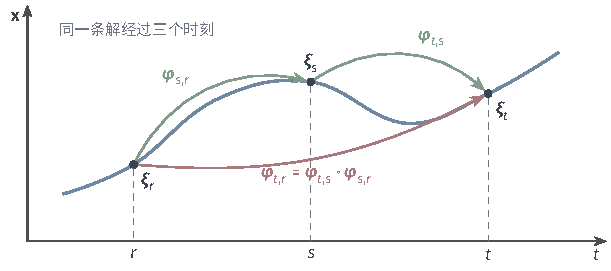
\includegraphics[width=100mm]{figures/03-optimization-evolution-and-signals/02-processes-and-trajectory-evolution/tikz/ode-flow-composition/figure.pdf}
  \caption{演化映射的复合关系示意。蓝色曲线是一条解在$(t,\bm x)$平面中的图像，它在时刻$r<s<t$分别经过$\bm\xi_r,\bm\xi_s,\bm\xi_t$。绿色箭头表示分两段传播$\bm\varphi_{s,r}$与$\bm\varphi_{t,s}$，红色箭头表示一次传播$\bm\varphi_{t,r}$；三者到达同一状态，是因为解唯一。}
  \label{fig:ode-flow-composition}
\end{figure}

\paragraph{自治方程的流}
向量场不显含时间时，规律不随时间改变，所以从$s$出发走$\tau$时间，与从$0$出发走$\tau$时间结果相同：若$\bm x$是从$(0,\bm\xi)$出发的解，则$\bm y(t)=\bm x(t-s)$满足$\dot{\bm y}(t)=\bm g(\bm y(t))$、$\bm y(s)=\bm\xi$，由唯一性它就是从$(s,\bm\xi)$出发的解。于是$\bm\varphi_{t,s}=\bm\varphi_{t-s,0}$只依赖时间差。

\begin{definition}[流]
  \label{def:ode-flow}
  设自治向量场$\bm g:D\to\mathbb R^d$局部Lipschitz，$J(\bm\xi)$是从$\bm x(0)=\bm\xi$出发的最大存在区间。映射$(t,\bm\xi)\mapsto\bm\varphi_t(\bm\xi)=\bm\varphi_{t,0}(\bm\xi)$（$t\in J(\bm\xi)$）称为$\bm g$的（局部）\term{流}。它满足$\bm\varphi_0=\mathrm{id}$，并在两边有定义时满足
  \begin{equation}
    \bm\varphi_{t+s}=\bm\varphi_t\circ\bm\varphi_s.
    \label{eq:ode-flow-group}
  \end{equation}
\end{definition}

式~\eqref{eq:ode-flow-group}由定理~\ref{thm:ode-evolution-composition}与时间平移得到。非自治方程没有这样的结构：$\dot x=tx$的解为$x(t)=\xi e^{(t^2-s^2)/2}$，于是$\bm\varphi_{1,0}(1)=e^{1/2}$，而同样经过一个单位时间的$\bm\varphi_{2,1}(1)=e^{3/2}$。规律本身随时间变化，传播效果就同时依赖起止两个时刻。

\paragraph{流把一团初值整体搬运}
固定$t$，流$\bm\varphi_t$把整个状态空间的点同时往前推$t$时间。与其一条一条地看轨迹，不如看一团初值被推成了什么形状。图~\ref{fig:ode-flow-deformation}从以$(-1,0)$为心、半径$0.35$的圆盘出发，画出它在$t=1.5,3,4.5$时的像。无阻尼摆把圆盘拉长、弯曲，但面积始终是$0.3848$，与初始圆盘相同；阻尼摆把圆盘越压越小，面积依次约为$0.2112$、$0.1159$、$0.0636$，恰好按$e^{-0.4t}$缩小。

\begin{figure*}[htbp]
  \centering
  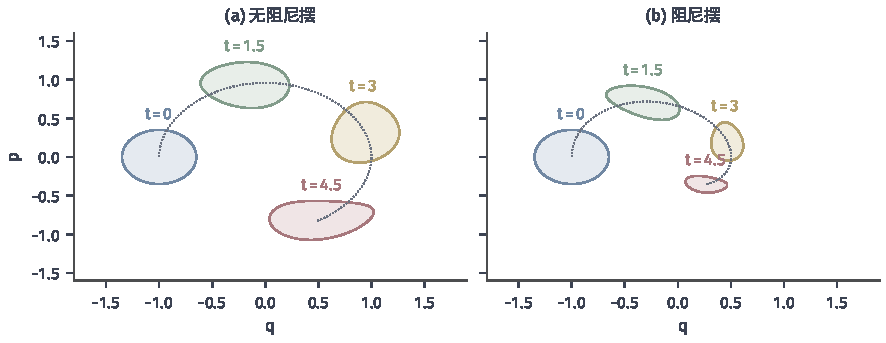
\includegraphics[width=150mm]{figures/03-optimization-evolution-and-signals/02-processes-and-trajectory-evolution/matplotlib/ode-flow-deformation/figure.pdf}
  \caption{流把一团初值整体搬运。初始集合是以$(-1,0)$为心、半径$0.35$的圆盘（蓝），依次画出它在$t=1.5$（绿）、$3$（黄）、$4.5$（红）时的像，点线是圆心的轨迹；边界由$400$个点分别积分得到。(a)无阻尼摆$\dot q=p$，$\dot p=-\sin q$：形状变化，面积保持$\pi\times0.35^2\approx0.3848$。(b)阻尼摆$\dot p=-\sin q-0.4p$：面积依次为$0.3848$、$0.2112$、$0.1159$、$0.0636$，与$0.3848e^{-0.4t}$一致。}
  \label{fig:ode-flow-deformation}
\end{figure*}

面积的变化由灵敏度矩阵控制。$\bm\varphi_t$在$\bm\xi$处的Jacobian矩阵就是定理~\ref{thm:ode-variational-equation}中的$\bm S(t)$，小区域的面积按$|\det\bm S(t)|$缩放。$\bm S$满足线性方程$\dot{\bm S}=\partial_{\bm x}\bm g\,\bm S$，第~\ref{sec:ode-time-varying-linear}小节将对这类方程证明$\det\bm S(t)=\exp\int_0^t\operatorname{tr}\partial_{\bm x}\bm g$。摆的$\partial_{\bm x}\bm g$的迹恒为$-c$，所以面积按$e^{-ct}$变化；无阻尼时迹为零，面积保持。这个观察是第~\ref{sec:ode-hamiltonian}节的起点。

\paragraph{局部流、正向全局与双向全局}
流是否对全部时间有定义，取决于最大存在区间。$\dot x=x^2$在$\xi>0$时$J(\xi)=(-\infty,1/\xi)$，在$\xi<0$时$J(\xi)=(1/\xi,\infty)$；对任何固定的$t>0$，$\bm\varphi_t$只在$\xi<1/t$上有定义，这种流称为局部流。

$\dot x=-x^3$的情形更微妙。由$\frac{\mathrm d}{\mathrm dt}x^{-2}=2$得$x(t)=\xi/\sqrt{1+2\xi^2t}$，它对全部$t\geq0$有定义，所以$\bm\varphi_t$对每个$t\geq0$在整条实轴上有定义，称为正向全局存在。反向时刻却只能退到$t>-1/(2\xi^2)$。经过时间$t$后，全部状态被压进区间$|x|<1/\sqrt{2t}$；这个区间之外的状态不是任何初值在$t$时间后的像。所以从$\bm\varphi_t(\xi)$恢复$\xi$总是可以的，只要沿原轨迹倒退；但随便指定一个状态往回推$t$时间，却可能在途中爆炸。逆向恢复需要相应方向的存在唯一。

若每个初值的最大解都在$(-\infty,\infty)$上存在，称流为全局流。这时每个$\bm\varphi_t$都是$\mathbb R^d$到自身的双射，逆映射是$\bm\varphi_{-t}$；常系数线性方程和摆都属于这种情形。下一节的状态转移矩阵是线性方程演化映射的矩阵表示，灵敏度矩阵则是非线性演化映射的一阶近似。

% 第8章第3节：典型方程的解析求解（可分离变量与标量线性方程；常系数线性系统；时变线性系统）。

\section{典型方程的解析求解}
\label{sec:ode-analytic-solutions}

上一节的理论说明解存在、唯一并连续依赖数据，却没有给出解的公式。本节处理能直接算出解的几类方程。每个公式都要同时核对两件事：它满足方程，也满足初值；它在哪个时间区间上成立。一般非线性方程没有闭式解，前一节的理论对它们照样适用，数值方法则在第~\ref{sec:ode-numerics}节处理。

\subsection{可分离变量方程与标量线性方程}
\label{sec:ode-separable-linear}

\paragraph{可分离变量方程}
若标量方程的右端可以写成时间因子与状态因子的乘积，
\begin{equation}
  \dot x=a(t)\,h(x),
  \label{eq:ode-separable}
\end{equation}
其中$a$在区间$I$上连续，$h$在开区间$D$上局部Lipschitz，就称它为可分离变量方程。形式上把$x$都移到一边、$t$移到另一边再积分，就得到解的隐式关系。下面说明这一操作何时合法。

先看$h(x_0)=0$的情形：常值函数$x\equiv x_0$满足方程与初值，由唯一性它就是解。这类解称为平衡解，在形式计算中两边除以$h(x)$时会被丢掉，必须单独列出。

再看$h(x_0)\neq0$的情形。这时解在整个最大存在区间上都满足$h(x(t))\neq0$：若某时刻$t_1$有$h(x(t_1))=0$，则常值函数$x\equiv x(t_1)$与$x$是从$(t_1,x(t_1))$出发的两个解，唯一性要求二者相同，与$h(x_0)\neq0$矛盾。于是$x(t)$始终留在包含$x_0$、使$h\neq0$的那个开区间$D_0$中。在$D_0$上令
\[
  G(x)=\int_{x_0}^x\frac{\mathrm d\xi}{h(\xi)},
\]
$G'=1/h$不变号，所以$G$严格单调。链式法则给出$\frac{\mathrm d}{\mathrm dt}G(x(t))=\dot x/h(x)=a(t)$，从$t_0$积分得
\begin{equation}
  G\bigl(x(t)\bigr)=\int_{t_0}^ta(s)\,\mathrm ds.
  \label{eq:ode-separable-implicit}
\end{equation}
$G$可逆，因此$x(t)=G^{-1}\bigl(\int_{t_0}^ta\bigr)$；这个式子在右端的积分落在$G$的值域内时成立，值域的端点正对应最大存在区间的端点。

\paragraph{时间等于路程除以速度}
取$a\equiv1$，式~\eqref{eq:ode-separable-implicit}变成
\[
  t-t_0=\int_{x_0}^{x(t)}\frac{\mathrm d\xi}{h(\xi)},
\]
即走过一段路程所需的时间等于路程元除以速度再累计。上一节的两个现象都可以从这个积分读出。若$h$在$+\infty$附近增长得足够快，使$\int_{x_0}^{\infty}\mathrm d\xi/h(\xi)<\infty$，解就在有限时间走到无穷远，这就是$\dot x=x^2$的爆炸。另一方面，若$h$在一个零点$x^\ast$附近满足Lipschitz条件，$|h(\xi)|\leq L|\xi-x^\ast|$，则$\int\mathrm d\xi/|h(\xi)|$在$x^\ast$附近像$\int\mathrm d\xi/|\xi-x^\ast|$一样发散，状态永远无法在有限时间到达平衡点，这与唯一性一致。$\dot x=\sqrt{|x|}$的反例恰好相反：$\int_0^1\mathrm d\xi/\sqrt\xi=2$有限，所以从原点出发到达$x=1$只需$2$个单位时间，平衡点可以在有限时间内被离开。

\begin{example}[Logistic方程]
  \label{ex:ode-logistic}
  考虑$\dot x=rx(1-x)$，$r>0$。平衡解是$x\equiv0$与$x\equiv1$。对$x_0\notin\{0,1\}$，部分分式给出$\int\mathrm d\xi/(\xi(1-\xi))=\log|\xi/(1-\xi)|$，式~\eqref{eq:ode-separable-implicit}化为$\log\left|\frac{x(1-x_0)}{x_0(1-x)}\right|=rt$。由于$x(t)$与$x_0$位于同一个$D_0$中，绝对值内的量为正，解出
  \[
    x(t)=\frac{x_0e^{rt}}{1-x_0+x_0e^{rt}}.
  \]
  对$x_0\in(0,1)$，分母恒正，解在全部时间存在并单调趋于$1$。对$x_0>1$，分母在$t=\frac1r\log\frac{x_0-1}{x_0}<0$处为零，所以解在过去某时刻从$+\infty$下来，正向全局存在。对$x_0<0$，分母在$t=\frac1r\log\frac{x_0-1}{x_0}>0$处为零，解在有限时间趋于$-\infty$。同一个公式在三种初值下给出三种存在区间，必须结合初值逐一判断。
\end{example}

隐式关系还可能需要选择分支。方程$\dot x=-t/x$定义在$D=(0,\infty)$上，$x(0)=x_0>0$。分离变量得$x\,\mathrm dx=-t\,\mathrm dt$，积分得$x^2+t^2=x_0^2$，这是一个圆。圆上有两个分支$x=\pm\sqrt{x_0^2-t^2}$，初值$x_0>0$选定上半支。解在$(-x_0,x_0)$上存在；在端点处$x\to0$，正是状态集合的边界，向量场$-t/x$在那里没有定义。圆的下半支是另一个初值问题的解，不能接在上半支后面。

\paragraph{积分因子与常数变易}
标量线性方程
\begin{equation}
  \dot x=-a(t)\,x+b(t),\qquad x(t_0)=x_0,
  \label{eq:ode-scalar-linear}
\end{equation}
其中$a,b$在$I$上连续，可以用积分因子求解。令$A(t)=\int_{t_0}^ta(s)\,\mathrm ds$，乘积法则给出$\frac{\mathrm d}{\mathrm dt}\bigl(e^{A(t)}x(t)\bigr)=e^{A(t)}\bigl(\dot x+a x\bigr)=e^{A(t)}b(t)$，积分后得到
\begin{equation}
  x(t)=e^{-A(t)}x_0+\int_{t_0}^te^{-(A(t)-A(s))}\,b(s)\,\mathrm ds.
  \label{eq:ode-scalar-variation}
\end{equation}
代入$t=t_0$得到初值，对$t$求导可验证方程，所以这确是解；由唯一性也是唯一的解。同一公式也可以这样得到：齐次方程$\dot x=-ax$的解是$Ce^{-A(t)}$，让常数$C$随时间变化，代入原方程得$\dot C=e^{A}b$，再积分。这一做法称为\term{常数变易}（variation of constants）。

式~\eqref{eq:ode-scalar-variation}把解分成两部分。第一项是初值的记忆，被因子$e^{-A(t)}$逐渐抹去；第二项是输入的累计，时刻$s$的输入在时刻$t$只剩下$e^{-(A(t)-A(s))}$的份额。对温度模型，$a\equiv\lambda$，$b=u$，
\[
  x(t)=e^{-\lambda(t-t_0)}x_0+\int_{t_0}^te^{-\lambda(t-s)}u(s)\,\mathrm ds.
\]
可以把它想象成：每一时刻送进的一小份热量$u(s)\,\mathrm ds$都以速率$\lambda$独立地散掉，此刻的温差是所有尚未散尽的份额之和。$\lambda=0.2$时，一份热量的半衰期是$\log2/0.2\approx3.47$分钟。恒定输入$u$下，积分算得$x(t)=u/\lambda+(x_0-u/\lambda)e^{-\lambda(t-t_0)}$：初值的作用消退，输入留下平衡值$u/\lambda$。“初值作用趋零”与“状态趋零”是两回事。

\begin{example}[周期加热的稳态响应]
  \label{ex:ode-periodic-heating}
  取$\lambda=0.2$，加热量在$0.4$上下摆动：$u(t)=0.4+0.2\sin\omega t$。试探形如$x_p(t)=2+\alpha\sin\omega t+\beta\cos\omega t$的解，代入方程并比较$\sin\omega t$与$\cos\omega t$的系数，得$\alpha\omega=-\lambda\beta$与$-\beta\omega=-\lambda\alpha+0.2$，解出
  \[
    \alpha=\frac{0.2\lambda}{\lambda^2+\omega^2},\qquad\beta=-\frac{0.2\omega}{\lambda^2+\omega^2}.
  \]
  所以$x_p(t)=2+\frac{0.2}{\sqrt{\lambda^2+\omega^2}}\sin(\omega t-\phi)$，其中$\phi=\arctan(\omega/\lambda)$。取$\omega=0.5$，振幅为$0.2/\sqrt{0.29}\approx0.371$，相位滞后约$1.19$弧度。一般解是$x_p$加上齐次解：$x(t)=x_p(t)+\bigl(x_0-x_p(0)\bigr)e^{-0.2t}$，其中$x_p(0)=2+\beta\approx1.655$。输入摆动越快，状态的摆动越小、越滞后：房间的热容把快速变化平滑掉了。
\end{example}

\paragraph{解析解作为数值基准}
解析解的价值不只在于给出公式。它让我们能精确核对一条轨迹的每个特征：平衡值、衰减速率、稳态振幅、爆炸时刻。第~\ref{sec:ode-numerics}节比较数值方法时，正是用这些公式算出“真值”，再测量误差随步长的变化；没有可核验的真值，就无法区分方法的误差与方程本身的行为。

\subsection{常系数线性系统}
\label{sec:ode-constant-linear}

\paragraph{矩阵指数}
标量方程$\dot x=ax$的解是$e^{at}x_0$。对向量方程$\dot{\bm x}=\bm A\bm x$，$\bm A\in\mathbb R^{d\times d}$，自然的猜测是用某种“矩阵的指数”代替$e^{at}$。指数函数的幂级数只用到乘法与加法，对方阵同样可以写出。矩阵指数在本书前置各卷中没有建立，这里从定义开始。

\begin{definition}[矩阵指数]
  \label{def:ode-matrix-exponential}
  对方阵$\bm A\in\mathbb R^{d\times d}$，定义\term{矩阵指数}
  \begin{equation}
    e^{\bm A}=\sum_{j=0}^\infty\frac{\bm A^j}{j!}=\bm I+\bm A+\frac{\bm A^2}{2!}+\cdots.
    \label{eq:ode-matrix-exponential}
  \end{equation}
\end{definition}

\begin{theorem}[矩阵指数的基本性质]
  \label{thm:ode-matrix-exponential-properties}
  设$\bm A,\bm B\in\mathbb R^{d\times d}$。
  \begin{enumerate}
    \item 级数~\eqref{eq:ode-matrix-exponential}绝对收敛；$\sum_jt^j\bm A^j/j!$在$t$的每个有界集合上一致收敛。
    \item $\frac{\mathrm d}{\mathrm dt}e^{t\bm A}=\bm Ae^{t\bm A}=e^{t\bm A}\bm A$。
    \item 若$\bm A\bm B=\bm B\bm A$，则$e^{\bm A+\bm B}=e^{\bm A}e^{\bm B}$。特别地，$e^{(t+s)\bm A}=e^{t\bm A}e^{s\bm A}$，并且$e^{t\bm A}$可逆，逆为$e^{-t\bm A}$。
    \item 若$\bm V$可逆，则$e^{\bm V\bm\Lambda\bm V^{-1}}=\bm Ve^{\bm\Lambda}\bm V^{-1}$。
  \end{enumerate}
\end{theorem}

\begin{proof}
  (1)取任一次乘性矩阵范数，例如谱范数，则$\|t^j\bm A^j/j!\|\leq(|t|\|\bm A\|)^j/j!$。右端是收敛的数值级数$e^{|t|\|\bm A\|}$的通项，在$|t|\leq T$上一致地被$(T\|\bm A\|)^j/j!$控制，由Weierstrass判别法得结论。

  (2)逐项求导得到级数$\sum_{j\geq1}t^{j-1}\bm A^j/(j-1)!=\bm A\sum_{i\geq0}t^i\bm A^i/i!$，由(1)它在有界区间上一致收敛，所以逐项求导合法。把$\bm A$提到右边也一样。

  (3)两个绝对收敛级数可以按Cauchy乘积相乘并重排：
  \[
    e^{\bm A}e^{\bm B}=\sum_{n\geq0}\sum_{j+k=n}\frac{\bm A^j\bm B^k}{j!\,k!}
    =\sum_{n\geq0}\frac1{n!}\sum_{j=0}^n\binom nj\bm A^j\bm B^{n-j}
    =\sum_{n\geq0}\frac{(\bm A+\bm B)^n}{n!}.
  \]
  最后一步是二项式展开，只有在$\bm A$与$\bm B$可交换时才成立。$t\bm A$与$s\bm A$可交换，取$s=-t$得$e^{t\bm A}e^{-t\bm A}=e^{\bm0}=\bm I$。

  (4)$(\bm V\bm\Lambda\bm V^{-1})^j=\bm V\bm\Lambda^j\bm V^{-1}$，逐项代入并提出$\bm V$与$\bm V^{-1}$。
\end{proof}

由(2)，$\bm x(t)=e^{(t-t_0)\bm A}\bm x_0$满足$\dot{\bm x}=\bm A\bm x$与初值；线性向量场关于状态全局Lipschitz，所以这就是唯一的解，并且对全部$t\in\mathbb R$存在。性质(3)中的可交换条件不能省略，第~\ref{sec:ode-time-varying-linear}小节会给出反例。

\paragraph{常数变易公式}
加入输入后，方程变为
\begin{equation}
  \dot{\bm x}(t)=\bm A\bm x(t)+\bm B\bm u(t),\qquad\bm x(t_0)=\bm x_0,
  \label{eq:ode-lti}
\end{equation}
其中$\bm B\in\mathbb R^{d\times m}$，$\bm u$局部可积。仿照标量情形，令$\bm z(t)=e^{-t\bm A}\bm x(t)$，乘积法则与性质(2)给出$\dot{\bm z}=e^{-t\bm A}(\dot{\bm x}-\bm A\bm x)=e^{-t\bm A}\bm B\bm u(t)$。积分并乘回$e^{t\bm A}$，得到
\begin{equation}
  \bm x(t)=e^{(t-t_0)\bm A}\bm x_0+\int_{t_0}^te^{(t-s)\bm A}\bm B\bm u(s)\,\mathrm ds.
  \label{eq:ode-lti-variation}
\end{equation}
代入$t=t_0$得初值；对上限求导可验证方程，局部可积输入下验证在几乎处处意义上成立。读法与标量情形相同：初态经过$e^{(t-t_0)\bm A}$传播，每一时刻的输入经过剩余时间$t-s$的传播后累加。

\paragraph{用特征方向读出相图}
$e^{t\bm A}$怎样作用，取决于$\bm A$的特征结构。若$\bm A$可对角化，$\bm A=\bm V\bm\Lambda\bm V^{-1}$，性质(4)给出$e^{t\bm A}=\bm Ve^{t\bm\Lambda}\bm V^{-1}$：把初态在特征向量基下展开，第$i$个坐标独立地乘以$e^{\lambda_it}$。实特征值$\lambda_i<0$的方向按指数收缩，$\lambda_i>0$的方向按指数伸长。一对共轭复特征值$\alpha\pm\mathrm i\beta$（$\beta\neq0$）对应一个二维实不变平面：若特征向量为$\bm v=\bm v_{\mathrm r}+\mathrm i\bm v_{\mathrm i}$，在基$\{\bm v_{\mathrm r},\bm v_{\mathrm i}\}$下$\bm A$的作用是$\begin{bmatrix}\alpha&\beta\\-\beta&\alpha\end{bmatrix}$，其指数为
\[
  e^{\alpha t}\begin{bmatrix}\cos\beta t&\sin\beta t\\-\sin\beta t&\cos\beta t\end{bmatrix},
\]
即一边以角速度$\beta$旋转、一边按$e^{\alpha t}$伸缩。实部决定靠近还是远离，虚部决定转得多快。

并非每个矩阵都有完整的特征向量基。若$\bm A$有Jordan块$\lambda\bm I+\bm N$，$\bm N$是幂零矩阵，则$\lambda\bm I$与$\bm N$可交换，性质(3)给出$e^{t(\lambda\bm I+\bm N)}=e^{\lambda t}\sum_{j<r}t^j\bm N^j/j!$，其中$r$是块的大小。指数因子之外多出了$t$的多项式。Jordan块及其幂中出现的多项式因子可参考\BookChapterRef{chap:linear-analysis}{卷一“谱和奇异值”章}。

图~\ref{fig:ode-phase-portraits}用二维例子把这些情形画出来。除(b)外，各图都是线性化的阻尼摆$\dot x_1=x_2$、$\dot x_2=-x_1-cx_2$，只改变阻尼系数$c$。特征方程$\lambda^2+c\lambda+1=0$给出$\lambda=\bigl(-c\pm\sqrt{c^2-4}\bigr)/2$。$c=2.5$时两个负实根$-0.5,-2$，轨迹不旋转地进入原点，并沿收缩较慢的方向$-0.5$贴近原点，称为稳定结点；$c=0.5$时一对实部为$-0.25$的复根，轨迹螺旋进入，称为稳定焦点；$c=0$时纯虚根$\pm\mathrm i$，轨迹是闭合的椭圆，称为中心；$c=-0.5$（负阻尼，相当于不断注入能量）时螺旋向外，称为不稳定焦点。$c=2$是临界情形：$\lambda=-1$是二重根，但$\bm A+\bm I=\begin{bmatrix}1&1\\-1&-1\end{bmatrix}$不为零而平方为零，只有一个特征方向$(1,-1)$，于是
\[
  e^{t\bm A}=e^{-t}\bigl(\bm I+t(\bm A+\bm I)\bigr)=e^{-t}\begin{bmatrix}1+t&t\\-t&1-t\end{bmatrix},
\]
轨迹都沿这唯一的方向进入原点，称为退化结点。(b)是倒立摆在顶点附近的线性化$\dot x_1=x_2$、$\dot x_2=x_1$，特征值$\pm1$，沿$(1,1)$方向伸长、沿$(1,-1)$方向收缩，称为鞍点。

\begin{figure*}[htbp]
  \centering
  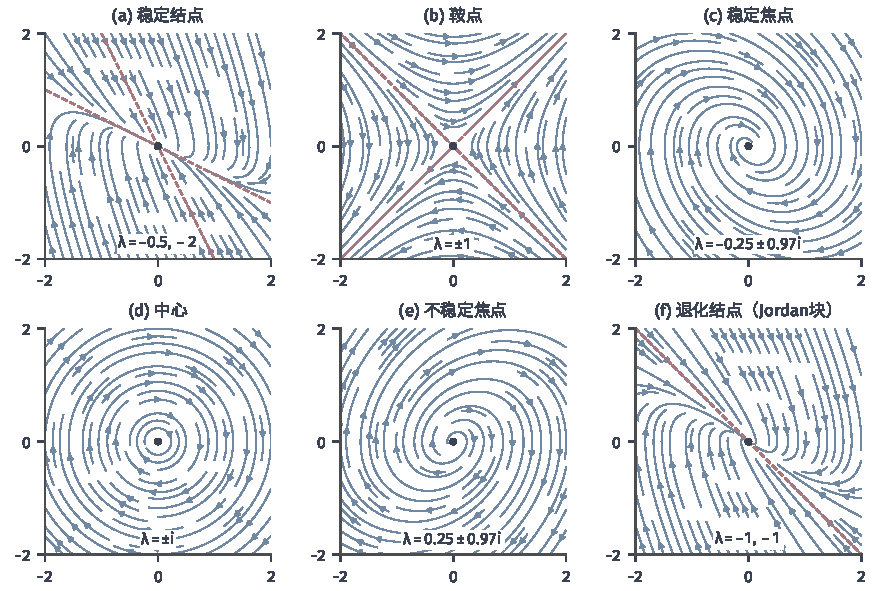
\includegraphics[width=150mm]{figures/03-optimization-evolution-and-signals/02-processes-and-trajectory-evolution/matplotlib/ode-phase-portraits/figure.pdf}
  \caption{二维常系数线性系统$\dot{\bm x}=\bm A\bm x$的相图。(a)(c)(d)(e)(f)取$\bm A=\begin{bmatrix}0&1\\-1&-c\end{bmatrix}$，阻尼系数依次为$c=2.5,0.5,0,-0.5,2$；(b)取$\bm A=\begin{bmatrix}0&1\\1&0\end{bmatrix}$。各图底部标出特征值，红色虚线是实特征向量方向（(f)只有一个）。流线由向量场绘制，箭头表示时间方向。}
  \label{fig:ode-phase-portraits}
\end{figure*}

一般的二阶矩阵可以按迹$\tau=\operatorname{tr}\bm A$与行列式$\Delta=\det\bm A$分类，因为特征值是$\bigl(\tau\pm\sqrt{\tau^2-4\Delta}\bigr)/2$：$\Delta<0$时为鞍点；$\Delta>0$且$\tau^2>4\Delta$时为结点；$\tau^2<4\Delta$时为焦点，$\tau=0$时退化为中心；$\tau^2=4\Delta$是分界情形，由是否可对角化决定是退化结点还是各方向等速收缩的星形结点。稳定与否由$\tau$的符号决定。这些画面在第~\ref{sec:ode-stability}节中用来判断非线性平衡点附近的行为。

\paragraph{分段常值输入下的精确离散}
计算机和控制器通常每隔$h$时间更新一次输入，在两次更新之间保持不变。设$\bm u(t)=\bm u_n$对$t\in[t_n,t_n+h)$成立。把式~\eqref{eq:ode-lti-variation}限制在这一段上，积分中的$\bm u$是常向量，可以提出：
\begin{equation}
  \bm x_{n+1}=\bm A_h\bm x_n+\bm B_h\bm u_n,\qquad
  \bm A_h=e^{h\bm A},\qquad
  \bm B_h=\int_0^he^{r\bm A}\,\mathrm dr\,\bm B,
  \label{eq:ode-zoh}
\end{equation}
其中$\bm x_n=\bm x(t_n)$，积分变量已换成$r=t_n+h-s$。这称为\term{零阶保持离散化}，它在输入确实分段常值时是精确的，与$h$大小无关。若$\bm A$可逆，$\int_0^he^{r\bm A}\,\mathrm dr=\bm A^{-1}(e^{h\bm A}-\bm I)$；$\bm A$奇异时应保留积分形式，或用分块矩阵一次算出两者：
\[
  \exp\left(h\begin{bmatrix}\bm A&\bm B\\\bm0&\bm0\end{bmatrix}\right)=\begin{bmatrix}\bm A_h&\bm B_h\\\bm0&\bm I\end{bmatrix}.
\]
这个等式的理由是：增广状态$(\bm x,\bm u)$满足$\dot{\bm x}=\bm A\bm x+\bm B\bm u$、$\dot{\bm u}=\bm0$，它在$h$时间后的状态既可以用分块矩阵的指数表示，也可以由式~\eqref{eq:ode-zoh}表示。

对温度模型，$\bm A=-\lambda$，$\bm B=1$，于是$a=e^{-\lambda h}$，$b=(1-e^{-\lambda h})/\lambda$。$\lambda=0.2$、$h=1$时$a\approx0.8187$，$b\approx0.9063$。冻结斜率的Euler近似则给出$a=1-\lambda h=0.8$，$b=h=1$。图~\ref{fig:ode-zoh-euler}取$h=2$以放大差别：前$10$分钟加热$0.4$，随后停止。精确离散的点（$a=e^{-0.4}\approx0.6703$，$b\approx1.6484$）恰好落在连续解上，$t=10$时都是$1.7293$；Euler的点（$a=0.6$，$b=2$）在加热阶段偏高，$t=10$时为$1.8445$，停止加热后又衰减过快，$t=20$时为$0.1434$，而真值是$0.2340$。

\begin{figure}[htbp]
  \centering
  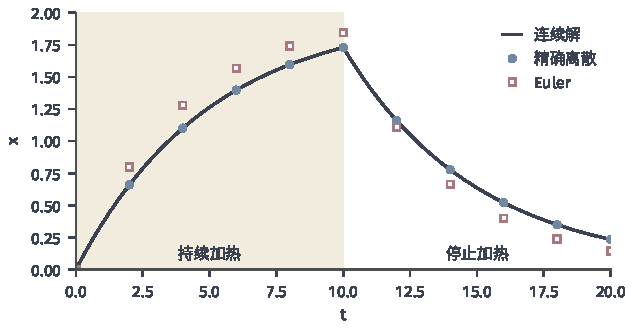
\includegraphics[width=107mm]{figures/03-optimization-evolution-and-signals/02-processes-and-trajectory-evolution/matplotlib/ode-zoh-euler/figure.pdf}
  \caption{分段常值输入下的精确离散与Euler近似。温度模型$\dot x=-0.2x+u$，$x(0)=0$，$u=0.4$（$0\leq t<10$，浅黄底）与$u=0$（$t\geq10$）。黑线为连续解；蓝点为步长$h=2$的零阶保持离散$x_{n+1}=e^{-0.4}x_n+1.6484\,u_n$，与连续解在采样时刻重合；红色方框为同一步长的Euler近似$x_{n+1}=0.6x_n+2u_n$。}
  \label{fig:ode-zoh-euler}
\end{figure}

反过来，从一个离散系数不能唯一推出连续模型。若已知离散模型$x_{n+1}=0.8x_n+u_n$，并把它看作步长$h=1$的Euler近似，对应$\lambda=0.2$、输入增益$1$；若看作零阶保持的精确采样，则需$e^{-\lambda}=0.8$，即$\lambda\approx0.2231$，而输入增益$\beta$须满足$\beta(1-0.8)/0.2231=1$，即$\beta\approx1.116$。两种解释给出不同的连续系统；若步长也未知，可能的连续模型还有无穷多个。此外，零阶保持的精确性依赖“输入在区间内不变”的约定；若真实输入在区间内线性变化，同样的$\bm A_h,\bm B_h$就不再精确。

\subsection{时变线性系统}
\label{sec:ode-time-varying-linear}

\paragraph{状态转移矩阵}
若系数随时间变化，$\dot{\bm x}=\bm A(t)\bm x$，标量情形的积分因子$e^{-\int a}$不能直接推广，原因稍后说明。可以换一个思路：不求公式，而把演化映射本身当作未知量。线性方程的演化映射是线性的，可以用矩阵表示。

\begin{definition}[状态转移矩阵]
  \label{def:ode-state-transition-matrix}
  设$\bm A:I\to\mathbb R^{d\times d}$连续。对$s\in I$，矩阵值函数$t\mapsto\bm\Phi(t,s)$若满足
  \begin{equation}
    \partial_t\bm\Phi(t,s)=\bm A(t)\bm\Phi(t,s),\qquad\bm\Phi(s,s)=\bm I,
    \label{eq:ode-state-transition}
  \end{equation}
  称为$\dot{\bm x}=\bm A(t)\bm x$的\term{状态转移矩阵}。
\end{definition}

$\bm\Phi(t,s)$的第$j$列是从$\bm x(s)=\bm e_j$出发的解，线性方程满足定理~\ref{thm:ode-global-existence}的增长条件，所以这些解在整个$I$上存在且唯一。由线性叠加，从任意$\bm x(s)=\bm\xi$出发的解是$\bm\Phi(t,s)\bm\xi$，即$\bm\Phi(t,s)$就是演化映射$\bm\varphi_{t,s}$的矩阵。

\begin{theorem}[状态转移矩阵的性质]
  \label{thm:ode-state-transition-properties}
  设$\bm A$与$\bm b$在$I$上连续。对$r,s,t\in I$：
  \begin{enumerate}
    \item $\bm\Phi(t,r)\bm\Phi(r,s)=\bm\Phi(t,s)$，并且$\bm\Phi(t,s)$可逆，$\bm\Phi(t,s)^{-1}=\bm\Phi(s,t)$；
    \item $\det\bm\Phi(t,s)=\exp\int_s^t\operatorname{tr}\bm A(\tau)\,\mathrm d\tau$；
    \item $\dot{\bm x}=\bm A(t)\bm x+\bm b(t)$、$\bm x(t_0)=\bm x_0$的解为
    \begin{equation}
      \bm x(t)=\bm\Phi(t,t_0)\bm x_0+\int_{t_0}^t\bm\Phi(t,s)\bm b(s)\,\mathrm ds.
      \label{eq:ode-ltv-variation}
    \end{equation}
  \end{enumerate}
\end{theorem}

\begin{proof}
  (1)是定理~\ref{thm:ode-evolution-composition}的矩阵形式：两边都是在时刻$r$等于$\bm\Phi(r,s)$的解。取$t=s$得$\bm\Phi(s,r)\bm\Phi(r,s)=\bm I$。

  (2)记$\bm\Phi(t)=\bm\Phi(t,s)$，$\delta(t)=\det\bm\Phi(t)$。行列式对每一行线性，所以$\dot\delta$等于把第$i$行换成其导数后的$d$个行列式之和。由$\dot{\bm\Phi}=\bm A\bm\Phi$，$\bm\Phi$第$i$行的导数是$\sum_kA_{i,k}(t)\times(\text{第}k\text{行})$；换入后，$k\neq i$的项含两个相同的行，行列式为零，只剩$A_{i,i}\delta$。求和得$\dot\delta=\operatorname{tr}\bm A(t)\,\delta$，$\delta(s)=1$，解这个标量线性方程即得结论。

  (3)对式~\eqref{eq:ode-ltv-variation}求导，积分上限给出$\bm\Phi(t,t)\bm b(t)=\bm b(t)$，被积函数对$t$求导给出$\bm A(t)\bm\Phi(t,s)\bm b(s)$，合起来是$\bm A(t)\bm x(t)+\bm b(t)$；代入$t=t_0$得初值。
\end{proof}

性质(2)称为Liouville公式，它把体积的变化与向量场的迹联系起来，第~\ref{sec:ode-flows}小节的面积计算和第~\ref{sec:ode-hamiltonian}节的体积保持都要用到它。它也说明$\bm\Phi(t,s)$总是可逆，与性质(1)一致。

\paragraph{时间次序不能交换}
标量情形$\Phi(t,s)=\exp\int_s^ta$，自然要问矩阵情形是否有$\bm\Phi(t,s)=\exp\int_s^t\bm A$。一般没有。取两个常矩阵
\[
  \bm A_1=\begin{bmatrix}0&1\\0&0\end{bmatrix},\qquad\bm A_2=\begin{bmatrix}0&0\\1&0\end{bmatrix},
\]
在$[0,1)$上$\bm A(t)=\bm A_1$，在$[1,2]$上$\bm A(t)=\bm A_2$（分段连续的系数，转移矩阵仍由分段求解拼接得到）。先运行$\bm A_1$一单位时间，再运行$\bm A_2$一单位时间，实际的传播是
\[
  \bm\Phi(2,0)=e^{\bm A_2}e^{\bm A_1}=\begin{bmatrix}1&0\\1&1\end{bmatrix}\begin{bmatrix}1&1\\0&1\end{bmatrix}=\begin{bmatrix}1&1\\1&2\end{bmatrix}.
\]
而$\int_0^2\bm A=\bm A_1+\bm A_2=\begin{bmatrix}0&1\\1&0\end{bmatrix}$，其指数为$\begin{bmatrix}\cosh1&\sinh1\\\sinh1&\cosh1\end{bmatrix}\approx\begin{bmatrix}1.543&1.175\\1.175&1.543\end{bmatrix}$，与真实传播不同。把顺序倒过来，$e^{\bm A_1}e^{\bm A_2}=\begin{bmatrix}2&1\\1&1\end{bmatrix}$又是第三个结果。几何上，$e^{\bm A_1}$是水平剪切，$e^{\bm A_2}$是竖直剪切，先做哪个会得到不同的形变；积分$\int\bm A$把整段时间的系数加在一起，丢掉了先后次序。

若对全部$t,s$都有$\bm A(t)\bm A(s)=\bm A(s)\bm A(t)$，次序就无关紧要，此时$\bm\Phi(t,s)=\exp\int_s^t\bm A$。理由是$\bm M(t)=\int_s^t\bm A$与它的导数$\bm A(t)$可交换，所以$\frac{\mathrm d}{\mathrm dt}\bm M^j=j\bm M^{j-1}\bm A(t)$，逐项求导得$\frac{\mathrm d}{\mathrm dt}e^{\bm M(t)}=\bm A(t)e^{\bm M(t)}$。标量方程和形如$\bm A(t)=a(t)\bm A_0$的系数都属于这种情形。

\paragraph{传播矩阵的计算与受迫响应}
除了可交换等特殊结构，$\bm\Phi(t,s)$一般没有闭式表达，需要求解$d\times d$个分量的矩阵初值问题~\eqref{eq:ode-state-transition}。是否值得这样做，取决于要回答的问题。若只要一条给定输入下的轨迹，直接对$\dot{\bm x}=\bm A(t)\bm x+\bm b(t)$作数值积分即可，只需一个$d$维初值问题。若要比较许多不同输入下的响应，或者要知道时刻$s$的一个单位脉冲在时刻$t$留下多少，就需要$\bm\Phi(t,s)$本身；对输出$\bm y=\bm C(t)\bm x$，式~\eqref{eq:ode-ltv-variation}说明输入到输出的历史核是$\bm C(t)\bm\Phi(t,s)\bm B(s)$，常系数时化为只依赖时间差的$\bm Ce^{(t-s)\bm A}\bm B$。

举一个可交换的例子：通风强度按一天的节律变化，散热系数为$\lambda(t)=0.2+0.1\sin(2\pi t/T_{\mathrm{day}})$。标量情形总可交换，$\Phi(t,s)=\exp\bigl(-\int_s^t\lambda\bigr)$，于是受迫响应$\int_{t_0}^t\Phi(t,s)u(s)\,\mathrm ds$中，同一份热量在通风强的时段散失得快、弱的时段散失得慢。一旦状态是多维的，并且各时刻的耦合矩阵不可交换，例如两个房间之间的换热随时间以不同方式改变，就只能数值地求$\bm\Phi$。

\paragraph{加权历史投影}
常系数与时变线性系统有一个重要用途：用有限维状态概括一整段输入历史。回到温度模型，取$x(0)=0$，常数变易公式给出
\[
  x(t)=\int_0^te^{-\lambda(t-s)}u(s)\,\mathrm ds.
\]
从另一个角度看，$x(t)$是输入历史在权函数$e^{-\lambda(t-s)}$下的加权累计，也就是历史在常数函数上的一个加权投影系数。它满足一个一维的微分方程，所以只用一个数就能随时更新这项历史特征。自然的问题是：若要保留更多的历史特征，例如加权平均之外的“趋势”，相应的系数能否仍然组成一个闭合的线性状态方程？

一般地，设要保留的系数为$c(t)=\int_{\alpha(t)}^{t}u(s)\psi(t,s)\,\mathrm ds$，其中$\psi$是基函数与权函数的乘积，积分窗口的左端$\alpha(t)$可以随时间移动。在$\psi$及其偏导数连续时，对上下限和被积函数求导的Leibniz法则给出
\begin{equation}
  \dot c(t)=u(t)\psi(t,t)-\dot\alpha(t)\,u\bigl(\alpha(t)\bigr)\psi\bigl(t,\alpha(t)\bigr)+\int_{\alpha(t)}^tu(s)\,\partial_t\psi(t,s)\,\mathrm ds.
  \label{eq:ode-history-leibniz}
\end{equation}
三项分别来自新输入进入窗口、旧输入离开窗口，以及窗口内部权重或基函数随时间改变。要得到闭合的状态方程，需要两点：第三项中的$\partial_t\psi$能写成已保留的基函数的线性组合；第二项要么不出现，要么能用已有系数表示。

\begin{example}[指数权下的闭合历史状态]
  \label{ex:ode-laguerre-history}
  取从$0$开始不断增长的窗口（$\alpha\equiv0$），以及基函数$\psi_k(t,s)=\frac{(t-s)^k}{k!}e^{-\lambda(t-s)}$，$k=0,1,\ldots,K-1$。令$c_k(t)=\int_0^tu(s)\psi_k(t,s)\,\mathrm ds$。由于$\psi_k(t,t)$在$k=0$时为$1$、$k\geq1$时为$0$，并且$\partial_t\psi_k=\psi_{k-1}-\lambda\psi_k$（$k\geq1$），$\partial_t\psi_0=-\lambda\psi_0$，式~\eqref{eq:ode-history-leibniz}给出
  \[
    \dot c_0=-\lambda c_0+u,\qquad\dot c_k=-\lambda c_k+c_{k-1}\quad(k\geq1).
  \]
  这是常系数线性系统$\dot{\bm c}=\bm A\bm c+\bm e_1u$，$\bm A=-\lambda\bm I+\bm N$，其中$\bm N$只在主对角线下方一条为$1$，所以$\bm A$恰是一个$K\times K$的Jordan块的转置。截断到前$K$项，方程仍然精确闭合：系数$c_0,\ldots,c_{K-1}$本身没有误差。误差只出现在用有限个系数重建输入历史的时候。
\end{example}

均匀权重的滑动窗口则不闭合。取窗口长度$T$，$c_0(t)=\frac1T\int_{t-T}^tu(s)\,\mathrm ds$，式~\eqref{eq:ode-history-leibniz}给出$\dot c_0=\bigl(u(t)-u(t-T)\bigr)/T$，需要$T$时间以前的输入值，而它不是任何已保留系数的函数。要精确地更新，就得保存整段窗口；有限维状态只能用已有系数重建出的近似值代替$u(t-T)$，这一步引入的余项不会因为系数方程是线性的而消失。

高阶多项式投影（high-order polynomial projection operators, HiPPO）框架系统地研究这类构造\scite{gu2020hippo}。其中一种取法把$[0,t]$上的均匀测度与缩放到$[0,t]$上的Legendre多项式作为权与基，得到时变线性方程$\dot{\bm c}=-\frac1t\bm A\bm c+\frac1t\bm Bu$，其中$A_{n,k}=\sqrt{2n+1}\sqrt{2k+1}$（$n>k$），$A_{n,n}=n+1$，$A_{n,k}=0$（$n<k$），$B_n=\sqrt{2n+1}$。它在截断后仍然闭合，原因与示例~\ref{ex:ode-laguerre-history}相同：基函数关于$t$的导数落在次数不更高的多项式张成的空间里。各时刻的系数矩阵都是同一个$\bm A$的倍数，彼此可交换，所以由上一段的结论，状态转移矩阵为$\bm\Phi(t,s)=\exp\bigl(-\log(t/s)\,\bm A\bigr)$。这里的$\tfrac1t$在$t=0$处奇异，初始状态须另行规定。投影坐标保存哪些历史特征由窗口、权和基共同决定；有限个系数逼近历史的误差、更新方程是否闭合，以及离散实现对扰动是否稳定，是三件需要分别核对的事。数值离散这些方程的方法统一放在第~\ref{sec:ode-numerics}节。

% 第8章第4节：稳定性与长期行为（平衡点、线性化与谱判据；Lyapunov函数与极限集合；持续输入下的轨迹响应）。

\section{稳定性与长期行为}
\label{sec:ode-stability}

第~\ref{sec:ode-continuous-dependence}小节的估计允许误差按$e^{Lt}$增长，只在有限时间内有用。实际关心的常常是另一类问题：房间最终是否稳定在某个温度，摆是否终将停下，微小的初值误差是越来越小还是越来越大。本节在同一个给定系统内依次研究三种情形：平衡点附近的小扰动，用谱和线性化判断；较大的区域乃至全空间，用Lyapunov函数与极限集合判断；持续存在的输入，用常数变易与含输入项的Lyapunov不等式估计状态范围。局部的线性判据与非线性的全局条件要分清，前者回答“离平衡足够近时”，后者回答“从这片区域出发时”。

本节只讨论自治方程$\dot{\bm x}=\bm g(\bm x)$，$\bm g$在开集$D$上局部Lipschitz；恒定输入已经代入$\bm g$。非自治情形需要把各项条件改为关于初始时刻一致成立，这里不展开。

\subsection{平衡点、线性化与谱判据}
\label{sec:ode-linear-stability}

\paragraph{平衡点与三种稳定}
满足$\bm g(\bm x^\ast)=\bm0$的状态$\bm x^\ast$称为\term{平衡点}（equilibrium）。从平衡点出发的解就是常值$\bm x^\ast$。温度模型在恒定加热$u$下的平衡点是$x^\ast=u/\lambda$；摆的平衡点是$(q,p)=(k\pi,0)$，偶数$k$对应摆锤在最低点，奇数$k$对应倒立。

真实系统不会恰好从平衡点出发。我们要问三件不同的事：小的初值偏差是否始终保持小；它是否最终消失；消失是否有统一的指数速度。

\begin{definition}[平衡点的稳定性]
  \label{def:ode-equilibrium-stability}
  设$\bm x^\ast$是$\dot{\bm x}=\bm g(\bm x)$的平衡点。
  \begin{enumerate}
    \item 若对每个$\varepsilon>0$存在$\delta>0$，使$\|\bm x_0-\bm x^\ast\|_2<\delta$时解对全部$t\geq0$存在并满足$\|\bm x(t)-\bm x^\ast\|_2<\varepsilon$，称$\bm x^\ast$在Lyapunov意义下\term{稳定}。
    \item 若存在$r>0$，使$\|\bm x_0-\bm x^\ast\|_2<r$时解对全部$t\geq0$存在并满足$\bm x(t)\to\bm x^\ast$，称$\bm x^\ast$是吸引的。稳定且吸引称为\term{渐近稳定}。
    \item 若存在$r,C,\alpha>0$，使$\|\bm x_0-\bm x^\ast\|_2<r$时解对全部$t\geq0$存在并满足
    \[
      \|\bm x(t)-\bm x^\ast\|_2\leq Ce^{-\alpha t}\|\bm x_0-\bm x^\ast\|_2,
    \]
    称$\bm x^\ast$\term{指数稳定}。
  \end{enumerate}
  若第2、3条对$D=\mathbb R^d$中的全部初值成立，相应地称为全局渐近稳定与全局指数稳定。不稳定指不满足第1条。
\end{definition}

这些定义都对一整个邻域里的初值下结论，并且要求解对全部未来存在；展示一条收敛的轨迹不能代替这样的量词。三个性质逐条加强，表~\ref{tab:ode-stability-types}用三个标量方程说明后一个确实比前一个多要求了东西。

\begin{table}[htbp]
  \centering
  \begin{tabular}{llll}
    \toprule
    方程 & 小偏差始终小 & 偏差趋于零 & 统一指数衰减\\
    \midrule
    $\dot x=0$ & 是，状态保持初值 & 否 & 否\\
    $\dot x=-x^3$ & 是，$|x(t)|$不增 & 是 & 否\\
    $\dot x=-x$ & 是 & 是 & 是\\
    \bottomrule
  \end{tabular}
  \caption{原点的三种稳定性质。$\dot x=-x^3$的解为$x(t)=x_0/\sqrt{1+2x_0^2t}$，按$t^{-1/2}$衰减，没有统一的指数速度；$\dot x=-x$的解为$e^{-t}x_0$。三个方程的解都对全部$t\geq0$存在。}
  \label{tab:ode-stability-types}
\end{table}

“稳定”与“吸引”控制的是不同的东西：前者限制轨迹在整个未来离平衡多远，后者只要求最终回来。所以渐近稳定的定义同时要求二者。指数稳定还要求衰减速率和常数$C$在整个邻域内统一，这一点在数值计算和输入响应估计中很重要，因为它使误差界可以写成具体的数。

\paragraph{线性系统的谱判据}
对线性系统$\dot{\bm x}=\bm A\bm x$，原点总是平衡点，并且解$e^{t\bm A}\bm x_0$关于初值线性，邻域的大小无关紧要：局部性质与全局性质相同。稳定性完全由$e^{t\bm A}$的长期行为决定，而上一节已经看到，$e^{t\bm A}$由特征值和Jordan结构决定。

\begin{theorem}[线性系统的谱判据]
  \label{thm:ode-linear-spectral-stability}
  设$\bm A\in\mathbb R^{d\times d}$。
  \begin{enumerate}
    \item $\dot{\bm x}=\bm A\bm x$的原点渐近稳定，当且仅当它全局指数稳定，当且仅当$\bm A$的全部特征值实部严格为负。这样的矩阵称为\term{Hurwitz矩阵}。
    \item 原点稳定，当且仅当全部特征值实部不大于零，并且实部为零的特征值对应的Jordan块都是$1\times1$的。
  \end{enumerate}
\end{theorem}

\begin{proof}
  在复数域写Jordan分解$\bm A=\bm V\bm J\bm V^{-1}$，于是$e^{t\bm A}=\bm Ve^{t\bm J}\bm V^{-1}$，只需对$\bm J$逐块研究。大小为$r$的块$\lambda\bm I+\bm N$的指数为$e^{\lambda t}\sum_{j<r}t^j\bm N^j/j!$，其各元素的模是$e^{t\operatorname{Re}\lambda}$乘以次数小于$r$的多项式。

  (1)若全部$\operatorname{Re}\lambda<0$，取$0<\alpha<\min_\lambda(-\operatorname{Re}\lambda)$。每个块都满足$e^{t\operatorname{Re}\lambda}t^j\leq C_je^{-\alpha t}$，有限个块合起来得$\|e^{t\bm A}\|\leq Ce^{-\alpha t}$，这就是全局指数稳定；它蕴含渐近稳定。反过来，若某个特征值$\lambda$满足$\operatorname{Re}\lambda\geq0$，取其特征向量$\bm v$，复解$e^{\lambda t}\bm v$的模不趋于零；它的实部和虚部都是实解，至少一个不趋于零，原点不是吸引的。

  (2)稳定等价于$\|e^{t\bm A}\|$在$t\geq0$上有界：有界时取$\delta=\varepsilon/\sup_t\|e^{t\bm A}\|$即可；无界时存在初值方向使解的范数任意大，按比例缩小初值也无法让它对所有$t$保持小。$\operatorname{Re}\lambda<0$的块有界；$\operatorname{Re}\lambda=0$的$1\times1$块$e^{\lambda t}$模为$1$，有界；$\operatorname{Re}\lambda=0$而块大小$r\geq2$时出现模为$t$的元素，无界；$\operatorname{Re}\lambda>0$时无界。
\end{proof}

两个判据的分界在虚轴上：严格在左半平面意味着指数衰减；落在虚轴上要看Jordan结构，可能稳定而不吸引（如中心），也可能多项式增长。例如$\bm A=\begin{bmatrix}0&1\\0&0\end{bmatrix}$的两个特征值都是零，但解$x_1(t)=x_1(0)+tx_2(0)$线性增长，原点不稳定。把严格不等号放宽成非严格不等号，结论就不再成立。

\paragraph{渐近衰减不等于单调下降}
Hurwitz条件保证$\|e^{t\bm A}\|\leq Ce^{-\alpha t}$，但常数$C$可能很大，状态在衰减之前可能先显著增长。取
\[
  \bm A=\begin{bmatrix}-1&K\\0&-2\end{bmatrix},\qquad K\geq0,
\]
特征值是$-1,-2$，与$K$无关。从$\bm x_0=(0,1)$出发，$x_2(t)=e^{-2t}$，而$x_1$满足$\dot x_1=-x_1+Ke^{-2t}$，解为$x_1(t)=K(e^{-t}-e^{-2t})$。$x_1$在$t=\log2$处达到最大值$K/4$。图~\ref{fig:ode-transient-growth}显示，$K=8$时状态范数从$1$升到约$2.02$，$K=20$时升到约$5.01$，此后才衰减。

\begin{figure*}[htbp]
  \centering
  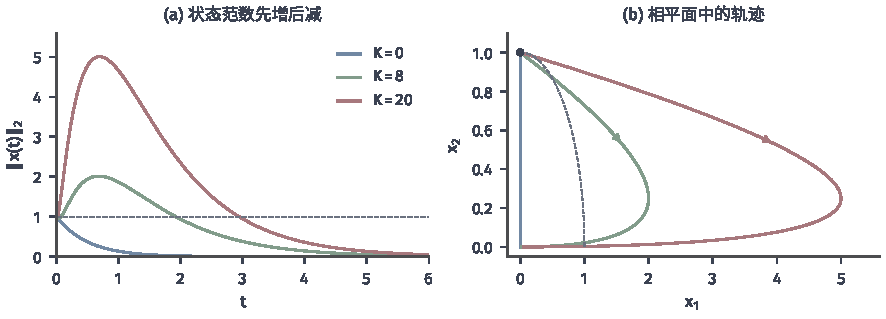
\includegraphics[width=150mm]{figures/03-optimization-evolution-and-signals/02-processes-and-trajectory-evolution/matplotlib/ode-transient-growth/figure.pdf}
  \caption{同谱系统的瞬态放大。$\bm A=\begin{bmatrix}-1&K\\0&-2\end{bmatrix}$，特征值恒为$-1,-2$，初值$(0,1)$。(a)状态的欧氏范数，$K=0,8,20$时峰值分别为$1$、约$2.02$、约$5.01$，灰色虚线为初始范数$1$。(b)相平面中的轨迹，灰色虚线为单位圆弧；$K>0$时轨迹先远离原点再返回。}
  \label{fig:ode-transient-growth}
\end{figure*}

放大来自第二个坐标向第一个坐标的单向耦合。$x_2$衰减的过程中不断向$x_1$输送“推力”，$x_1$来不及衰减就被推高。$K\neq0$时$\bm A\bm A^\top\neq\bm A^\top\bm A$，这类矩阵称为非正规矩阵；它的特征向量$(1,0)$与$(K,-1)$在$K$大时几乎共线，特征值只描述了最终的衰减速率，没有描述特征方向之间的几何关系。

何时会出现增长，可以直接从欧氏范数的导数判断：
\[
  \frac{\mathrm d}{\mathrm dt}\frac12\|\bm x\|_2^2=\bm x^\top\bm A\bm x=\bm x^\top\bm S\bm x,\qquad\bm S=\frac{\bm A+\bm A^\top}2.
\]
所以范数对一切初值都单调不增，当且仅当对称部分$\bm S$半负定。本例$\bm S$的最大特征值为$\bigl(-3+\sqrt{1+K^2}\bigr)/2$，$K>2\sqrt2$时为正，存在一些初始方向使范数先增长。谱判据说明“最终会回来”，对称部分说明“此刻是否在靠近”，二者回答的问题不同。下面的Lyapunov方程表明，换一个合适的二次型度量距离，就能让每条轨迹都单调靠近原点。

\paragraph{Lyapunov方程}
若欧氏距离不单调，不妨找一个椭圆形的度量：$V(\bm x)=\bm x^\top\bm P\bm x$，$\bm P\succ\bm0$。沿解有$\dot V=\bm x^\top(\bm A^\top\bm P+\bm P\bm A)\bm x$。要求它对一切非零$\bm x$为负，就是要求$\bm A^\top\bm P+\bm P\bm A$负定。

\begin{theorem}[连续时间Lyapunov方程]
  \label{thm:ode-lyapunov-equation}
  $\bm A$为Hurwitz矩阵，当且仅当对每个对称正定的$\bm Q$，存在唯一的对称正定$\bm P$满足
  \begin{equation}
    \bm A^\top\bm P+\bm P\bm A=-\bm Q.
    \label{eq:ode-lyapunov-equation}
  \end{equation}
\end{theorem}

\begin{proof}
  设$\bm A$为Hurwitz矩阵，令$\bm P=\int_0^\infty e^{t\bm A^\top}\bm Qe^{t\bm A}\,\mathrm dt$。由定理~\ref{thm:ode-linear-spectral-stability}，被积函数按$e^{-2\alpha t}$衰减，积分收敛。对非零$\bm x$，
  \[
    \bm x^\top\bm P\bm x=\int_0^\infty(e^{t\bm A}\bm x)^\top\bm Q(e^{t\bm A}\bm x)\,\mathrm dt>0,
  \]
  所以$\bm P\succ\bm0$。被积函数对$t$的导数是$\bm A^\top(\cdot)+(\cdot)\bm A$，积分得$\bm A^\top\bm P+\bm P\bm A=\bigl[e^{t\bm A^\top}\bm Qe^{t\bm A}\bigr]_0^\infty=-\bm Q$。若另有解，两解之差$\bm D$满足$\bm A^\top\bm D+\bm D\bm A=\bm0$，于是$\frac{\mathrm d}{\mathrm dt}\bigl(e^{t\bm A^\top}\bm De^{t\bm A}\bigr)=\bm0$，即$e^{t\bm A^\top}\bm De^{t\bm A}=\bm D$；令$t\to\infty$得$\bm D=\bm0$。

  反过来，设$\bm P,\bm Q\succ\bm0$满足方程。记$p_-,p_+$为$\bm P$的最小、最大特征值，$q_-$为$\bm Q$的最小特征值，则$p_-\|\bm x\|_2^2\leq V\leq p_+\|\bm x\|_2^2$，并且$\dot V=-\bm x^\top\bm Q\bm x\leq-q_-\|\bm x\|_2^2\leq-(q_-/p_+)V$。于是$\frac{\mathrm d}{\mathrm dt}\bigl(e^{(q_-/p_+)t}V\bigr)\leq0$，得$V(t)\leq e^{-(q_-/p_+)t}V(0)$，从而
  \[
    \|\bm x(t)\|_2\leq\sqrt{p_+/p_-}\;e^{-q_-t/(2p_+)}\|\bm x_0\|_2.
  \]
  这是全局指数稳定，由定理~\ref{thm:ode-linear-spectral-stability}，$\bm A$为Hurwitz矩阵。
\end{proof}

\begin{example}[手算Lyapunov方程]
  \label{ex:ode-lyapunov-equation}
  取$\bm A=\begin{bmatrix}0&1\\-2&-3\end{bmatrix}$，特征值$-1,-2$。令$\bm Q=\bm I$，$\bm P=\begin{bmatrix}p&q\\q&r\end{bmatrix}$，方程~\eqref{eq:ode-lyapunov-equation}的三个独立分量为$-4q=-1$、$p-3q-2r=0$、$2q-6r=-1$，解得$q=r=\tfrac14$，$p=\tfrac54$。$\bm P$的特征值约为$1.309$与$0.191$，确实正定。由上面的估计，$\|\bm x(t)\|_2$的上界按$e^{-t/(2\times1.309)}\approx e^{-0.38t}$衰减。这是一个保证，比最慢模态的真实速率$e^{-t}$保守。另一方面，$\bm A$的对称部分$\begin{bmatrix}0&-1/2\\-1/2&-3\end{bmatrix}$有正特征值约$0.081$，所以欧氏范数并非对一切初值单调下降，而$\bm P$给出的椭圆度量却是单调的。
\end{example}

图~\ref{fig:ode-lyapunov-levels}(a)画出这个例子：黄色椭圆是$V=\bm x^\top\bm P\bm x$的等值线，蓝色轨迹每穿过一条椭圆都由外向内，从不回头。线性系统因此总能为稳定的动力学找到一个二次“能量”，只是这个能量一般不是欧氏范数的平方。

\paragraph{非线性系统的局部线性化}
在平衡点附近，光滑向量场近似于它的线性部分。设$\bm g$在$\bm x^\ast$附近连续可微，记Jacobian矩阵$\bm J=\partial\bm g(\bm x^\ast)$，偏差$\bm e=\bm x-\bm x^\ast$满足
\[
  \dot{\bm e}=\bm J\bm e+\bm\rho(\bm e),\qquad\|\bm\rho(\bm e)\|_2\leq\epsilon(r)\|\bm e\|_2\quad(\|\bm e\|_2\leq r),
\]
其中$\epsilon(r)\to0$（$r\to0$），这正是可微性的定义。问题是：高阶项$\bm\rho$会不会改变线性部分给出的结论？

\begin{theorem}[线性化判据]
  \label{thm:ode-linearization}
  设$\bm g$在平衡点$\bm x^\ast$的邻域内连续可微，$\bm J=\partial\bm g(\bm x^\ast)$。
  \begin{enumerate}
    \item 若$\bm J$为Hurwitz矩阵，则$\bm x^\ast$局部指数稳定。
    \item 若$\bm J$有实部为正的特征值，则$\bm x^\ast$不稳定。
  \end{enumerate}
\end{theorem}

\begin{proof}
  (1)由定理~\ref{thm:ode-lyapunov-equation}取$\bm P\succ\bm0$满足$\bm J^\top\bm P+\bm P\bm J=-\bm I$，令$V(\bm e)=\bm e^\top\bm P\bm e$。沿解，
  \[
    \dot V=-\|\bm e\|_2^2+2\bm e^\top\bm P\bm\rho(\bm e)\leq-\bigl(1-2p_+\epsilon(r)\bigr)\|\bm e\|_2^2\qquad(\|\bm e\|_2\leq r).
  \]
  取$r$足够小，使$2p_+\epsilon(r)\leq\tfrac12$且闭球在邻域内，则$\dot V\leq-\tfrac12\|\bm e\|_2^2\leq-V/(2p_+)$。集合$\{V<p_-r^2\}$包含在半径$r$的球内；从其中出发的解，$V$沿途不增，所以不能离开这个集合，由定理~\ref{thm:ode-escape}对全部$t\geq0$存在。与上一定理的证明相同，得$\|\bm e(t)\|_2\leq\sqrt{p_+/p_-}\,e^{-t/(4p_+)}\|\bm e(0)\|_2$。

  (2)的证明构造一个在不稳定方向上增长的二次函数，论证与(1)类似但更长，这里引用其结论。
\end{proof}

第(2)条的完整证明见Khalil的非线性系统教材\scite{math-khalil2002nonlinear}。线性化给出的是局部结论：它只说明从足够近处出发的轨迹回到平衡点，不说明“足够近”有多近。若$\bm J$的特征值落在虚轴上而其余都在左半平面，线性化无法判断，高阶项决定结果。$\dot x=-x^3$与$\dot x=x^3$在原点的线性化都是$0$，前者渐近稳定，后者的解$x_0/\sqrt{1-2x_0^2t}$在有限时间爆炸，原点不稳定。

回到摆。最低点$(0,0)$处$\bm J=\begin{bmatrix}0&1\\-1&-c\end{bmatrix}$，$c>0$时为Hurwitz矩阵，最低点局部指数稳定；$c=0$时特征值为$\pm\mathrm i$，线性化无法判断，下一小节用能量说明它稳定但不吸引。倒立点$(\pi,0)$处$\bm J=\begin{bmatrix}0&1\\1&-c\end{bmatrix}$，行列式为$-1<0$，有一个正特征值，是鞍点，不稳定。这些局部画面正是图~\ref{fig:ode-phase-portraits}中的焦点、中心与鞍点。

\paragraph{虚轴与单位圆}
第~\ref{chap:discrete-dynamical-systems}章的离散线性系统$\bm x_{n+1}=\bm M\bm x_n$以单位圆为界：全部特征值的模小于$1$时渐近稳定。连续时间的界是虚轴。两者通过指数映射对应：步长为$h$的精确采样给出$\bm M=e^{h\bm A}$，其特征值为$e^{h\lambda}$，模为$e^{h\operatorname{Re}\lambda}$，于是$\operatorname{Re}\lambda<0$恰好对应$|e^{h\lambda}|<1$。精确采样保持稳定性；近似的离散化却未必。Euler近似给出$\bm M=\bm I+h\bm A$，特征值为$1+h\lambda$，它落在单位圆内要求$h\lambda$落在以$-1$为心的单位圆盘内，例如$\lambda=-0.2$时要求$h<10$。离散与连续的稳定条件不能套用同一个不等式，第~\ref{sec:ode-stiff}小节将系统研究这一点。

\subsection{Lyapunov函数与极限集合}
\label{sec:ode-lyapunov}

\paragraph{沿轨迹的变化率}
线性化只看平衡点的一个小邻域。要对更大的区域下结论，可以模仿Lyapunov方程中的做法：找一个标量函数$V$度量“离平衡有多远”，再证明它沿每条轨迹下降。关键在于不需要求出轨迹就能计算这个下降速率。若$V$连续可微，链式法则给出
\[
  \frac{\mathrm d}{\mathrm dt}V\bigl(\bm x(t)\bigr)=\nabla V\bigl(\bm x(t)\bigr)^\top\bm g\bigl(\bm x(t)\bigr).
\]
右端只依赖当前状态，于是定义$\dot V(\bm x)=\nabla V(\bm x)^\top\bm g(\bm x)$，它是$V$的梯度与向量场的内积。几何上，把$V$的等值线画在相平面上：$\dot V<0$意味着向量场在每一点都指向$V$更小的一侧，轨迹只能一层一层地穿过等值线向内走。

以原点为平衡点，称$C^1$函数$V$在原点的邻域$U$内正定，若$V(\bm0)=0$且$V(\bm x)>0$对$\bm x\in U\setminus\{\bm0\}$成立。正定只是形状上的要求，说明“$V$小”意味着“离原点近”；它还没有说明$V$沿轨迹怎样变化。

\begin{definition}[Lyapunov函数]
  \label{def:ode-lyapunov-function}
  设原点是$\dot{\bm x}=\bm g(\bm x)$的平衡点，$V$在原点的邻域$U$内连续可微且正定。若$\dot V(\bm x)\leq0$对$\bm x\in U$成立，称$V$为$U$上的\term{Lyapunov函数}；若$\dot V(\bm x)<0$对$\bm x\in U\setminus\{\bm0\}$成立，称为严格Lyapunov函数。
\end{definition}

\begin{theorem}[连续时间Lyapunov判据]
  \label{thm:ode-lyapunov}
  \label{thm:dynamical-nonlinear-lyapunov}
  设原点是$\dot{\bm x}=\bm g(\bm x)$的平衡点，$\bm g$在原点的邻域$U$内局部Lipschitz。
  \begin{enumerate}
    \item 若$U$上存在Lyapunov函数，则原点稳定。
    \item 若$U$上存在严格Lyapunov函数，则原点渐近稳定。
    \item 若$U=\mathbb R^d$，$V$在$\mathbb R^d$上正定、径向无界（即$\|\bm x\|_2\to\infty$时$V(\bm x)\to\infty$），并且$\dot V\leq0$，则每条解对全部$t\geq0$存在且原点稳定；若进而$\dot V(\bm x)<0$对一切$\bm x\neq\bm0$成立，则原点全局渐近稳定。
  \end{enumerate}
\end{theorem}

\begin{proof}
  (1)取$\varepsilon>0$足够小，使闭球$\bar B_\varepsilon=\{\|\bm x\|_2\leq\varepsilon\}\subseteq U$。$V$在球面$\|\bm x\|_2=\varepsilon$上连续且为正，有正的最小值$c_\varepsilon$。$V$在原点连续且$V(\bm0)=0$，故存在$\delta\in(0,\varepsilon)$使$\|\bm x_0\|_2<\delta$时$V(\bm x_0)<c_\varepsilon$。从这样的$\bm x_0$出发，只要轨迹留在$\bar B_\varepsilon$中，$V$就不增，始终小于$c_\varepsilon$；而要离开球，轨迹必须先到达球面，那里$V\geq c_\varepsilon$，矛盾。于是轨迹留在紧集$\bar B_\varepsilon$中，由定理~\ref{thm:ode-escape}对全部$t\geq0$存在，且$\|\bm x(t)\|_2<\varepsilon$，这就是稳定性。

  (2)沿用(1)中的轨迹。$V(\bm x(t))$单调不增且非负，有极限$v_\infty\geq0$。若$v_\infty>0$，由$V$的连续性，存在$\eta>0$使$\|\bm x(t)\|_2\geq\eta$对全部$t$成立（否则轨迹会任意接近原点，$V$也会任意接近$0$）。在紧集$\{\eta\leq\|\bm x\|_2\leq\varepsilon\}$上连续函数$-\dot V$有正的最小值$\kappa$，于是$V(\bm x(t))\leq V(\bm x_0)-\kappa t$，$t$大时为负，矛盾。故$v_\infty=0$。最后，若$\bm x(t)$不趋于零，则有$\eta'>0$与$t_j\to\infty$使$\|\bm x(t_j)\|_2\geq\eta'$，从而$V(\bm x(t_j))\geq\min_{\eta'\leq\|\bm x\|_2\leq\varepsilon}V>0$，与$v_\infty=0$矛盾。

  (3)径向无界保证每个子水平集$\{V\leq V(\bm x_0)\}$有界，它又是闭集，所以紧。轨迹的$V$不增，因而留在这个紧集中，对全部$t\geq0$存在。稳定性同(1)。严格下降时，把(2)中的球$\bar B_\varepsilon$换成这个子水平集，同样的论证对任意初值成立。
\end{proof}

为什么全局结论需要径向无界？若$V$在远处趋于一个有限值，它的某些子水平集就无界，轨迹可以一边让$V$下降，一边沿着无界的子水平集跑向无穷。只在原点附近正定，控制不了远处的状态。

\begin{example}[线性化失效而Lyapunov函数有效]
  \label{ex:ode-lyapunov-cubic}
  考虑$\dot x_1=-x_1^3+x_2$，$\dot x_2=-x_1-x_2^3$。原点的Jacobian矩阵为$\begin{bmatrix}0&1\\-1&0\end{bmatrix}$，特征值$\pm\mathrm i$，定理~\ref{thm:ode-linearization}无法判断。取$V=(x_1^2+x_2^2)/2$，则
  \[
    \dot V=x_1(-x_1^3+x_2)+x_2(-x_1-x_2^3)=-x_1^4-x_2^4,
  \]
  在原点之外严格为负；$V$正定且径向无界。由定理~\ref{thm:ode-lyapunov}，原点全局渐近稳定。衰减却不是指数的：$\dot V\geq-(x_1^2+x_2^2)^2=-4V^2$，所以$V(t)\geq V_0/(1+4V_0t)$，只按$1/t$减小。
\end{example}

若还能找到常数$c_1,c_2,c_3>0$使$c_1\|\bm x\|_2^2\leq V\leq c_2\|\bm x\|_2^2$且$\dot V\leq-c_3\|\bm x\|_2^2$，Lyapunov方程证明中的积分估计照样适用，给出指数稳定。一般的严格下降没有这种二次比较，上例就是渐近稳定而不指数稳定的情形。

\paragraph{不变集与$\omega$极限集}
许多物理系统的能量只在部分方向上耗散。阻尼摆的机械能$V=p^2/2+(1-\cos q)$满足$\dot V=-cp^2$，在整条直线$p=0$上为零，所以$V$只是非严格的Lyapunov函数，定理~\ref{thm:ode-lyapunov}的(2)用不上。可是直觉上摆终将停下：轨迹即使碰到$p=0$，也会被重力立刻推离。要把这一直觉写成证明，需要描述“轨迹最终停留在哪里”。

\begin{definition}[不变集与$\omega$极限集]
  \label{def:ode-invariant-limit-sets}
  \label{def:dynamical-invariant-limit-sets}
  设$\bm\varphi_t$是局部Lipschitz自治方程的流。
  \begin{enumerate}
    \item 若从$\Omega$中每一点出发的解对全部$t\geq0$存在且$\bm\varphi_t(\Omega)\subseteq\Omega$，称$\Omega$为\term{正向不变集}。
    \item 若从$M$中每一点出发的解对全部$t\in\mathbb R$存在且$\bm\varphi_t(M)=M$对全部$t\geq0$成立，称$M$为\term{不变集}。等价地，$M$中每一点都位于一条始终留在$M$中的完整轨迹上。
    \item 设从$\bm x_0$出发的解对全部$t\geq0$存在。它的\term{$\omega$极限集}是
    \[
      \omega(\bm x_0)=\bigl\{\bm z:\text{存在}t_j\to\infty\text{使}\bm x(t_j)\to\bm z\bigr\}.
    \]
  \end{enumerate}
\end{definition}

正向不变集限制一批初值的全部未来；$\omega$极限集记录一条轨迹在越来越晚的时刻反复靠近的状态。趋于平衡点的轨迹，其$\omega$极限集就是这个点；绕着闭曲线越转越近的轨迹，其$\omega$极限集是整条闭曲线。轨迹“趋于”一个集合，指它到该集合的距离趋于零，不要求它在集合中停下。

\begin{lemma}[$\omega$极限集的性质]
  \label{lem:ode-omega-limit}
  设从$\bm x_0$出发的解对全部$t\geq0$存在，并始终留在紧集$K\subseteq D$中。则$\omega(\bm x_0)$非空、紧、不变，并且$\operatorname{dist}\bigl(\bm x(t),\omega(\bm x_0)\bigr)\to0$。
\end{lemma}

\begin{proof}
  \emph{非空与紧。}由紧性，序列$\bm x(j)$有收敛子列，其极限属于$\omega(\bm x_0)$。$\omega(\bm x_0)\subseteq K$有界；它也是闭集：若$\bm z_k\in\omega(\bm x_0)$收敛到$\bm z$，对每个$k$取$t_k>k$使$\|\bm x(t_k)-\bm z_k\|_2<1/k$，则$\bm x(t_k)\to\bm z$。

  \emph{不变。}设$\bm z=\lim_j\bm x(t_j)\in\omega(\bm x_0)$，固定$s\geq0$。由定理~\ref{thm:ode-continuous-dependence}（在紧集$K$的一个紧邻域上取Lipschitz常数），流在有限时间$s$内连续依赖初值，故$\bm x(t_j+s)=\bm\varphi_s(\bm x(t_j))\to\bm\varphi_s(\bm z)$，即$\bm\varphi_s(\bm z)\in\omega(\bm x_0)$。反方向，$j$充分大时$t_j>s$，由紧性可从$\bm x(t_j-s)$中取出收敛子列，其极限$\bm w$属于$\omega(\bm x_0)$，并且$\bm\varphi_s(\bm w)=\lim\bm x(t_j)=\bm z$。所以$\bm\varphi_s(\omega(\bm x_0))=\omega(\bm x_0)$；从$\bm z$出发向过去的解可由这样的$\bm w$逐段拼出，始终在$\omega(\bm x_0)$中。

  \emph{吸引。}若距离不趋于零，则有$\varepsilon>0$与$t_j\to\infty$使$\operatorname{dist}(\bm x(t_j),\omega(\bm x_0))\geq\varepsilon$。紧性给出收敛子列，其极限属于$\omega(\bm x_0)$，与距离下界矛盾。
\end{proof}

\paragraph{LaSalle不变性原理}
有了$\omega$极限集，非严格下降的问题可以这样处理：$V$沿轨迹单调有下界，最终趋于一个常数，所以在$\omega$极限集上$V$恒为这个常数，$\dot V$在那里为零；而$\omega$极限集又是不变的。于是只需在$\dot V=0$的集合里找出“能整条轨迹待在里面”的部分。

\begin{theorem}[LaSalle不变性原理]
  \label{thm:ode-lasalle}
  设$\Omega\subseteq D$紧且正向不变，$V$在包含$\Omega$的开集上连续可微，并在$\Omega$上满足$\dot V\leq0$。令$E=\{\bm x\in\Omega:\dot V(\bm x)=0\}$，$M$为$E$中所含的最大不变集。则从$\Omega$出发的每条解满足$\operatorname{dist}(\bm x(t),M)\to0$（$t\to\infty$）。
\end{theorem}

\begin{proof}
  解留在紧集$\Omega$中，由引理~\ref{lem:ode-omega-limit}，$\omega(\bm x_0)\subseteq\Omega$非空、不变，并且轨迹趋于它。$V(\bm x(t))$不增且在紧集上有下界，趋于某个$v_\infty$；由连续性，$V$在$\omega(\bm x_0)$上恒等于$v_\infty$。从$\omega(\bm x_0)$中一点出发的解留在其中，沿它$V$为常数，所以$\dot V=0$，即$\omega(\bm x_0)\subseteq E$。不变的$\omega(\bm x_0)$因而包含在$M$中，轨迹趋于$\omega(\bm x_0)$，也就趋于$M$。
\end{proof}

\begin{example}[阻尼摆停在最低点]
  \label{ex:ode-damped-pendulum-lasalle}
  阻尼摆$\dot q=p$，$\dot p=-\sin q-cp$，$c>0$，取机械能$V=p^2/2+1-\cos q$，则$\dot V=p(-\sin q-cp)+p\sin q=-cp^2\leq0$。固定$v_0<2$，令$\Omega=\{(q,p):|q|\leq\arccos(1-v_0),\ V\leq v_0\}$。它是$\{V\leq v_0\}$中包含原点的那一块，有界闭，并且与其他块（围绕$q=\pm2\pi,\ldots$）不相连；$V$不增与轨迹的连续性使轨迹不能离开它，所以$\Omega$紧且正向不变。零导数集$E$是$\Omega$中$p=0$的部分。若一条完整轨迹始终在$E$中，则$p\equiv0$，于是$\dot p=-\sin q=0$，在$|q|<\pi$内只能$q=0$。所以$M=\{(0,0)\}$，从$\Omega$出发的轨迹都趋于最低点。
\end{example}

\begin{figure*}[htbp]
  \centering
  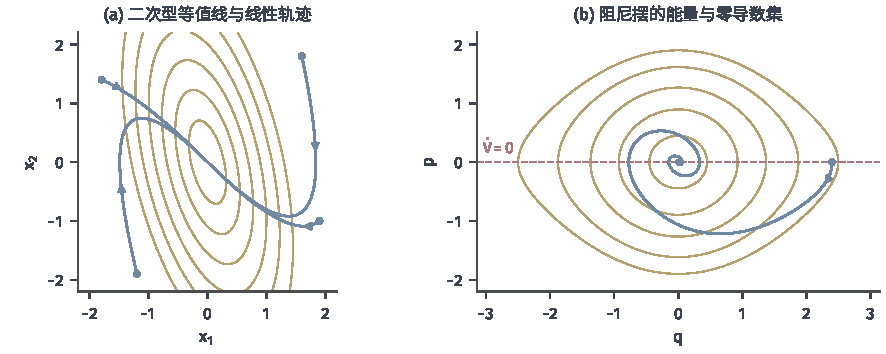
\includegraphics[width=150mm]{figures/03-optimization-evolution-and-signals/02-processes-and-trajectory-evolution/matplotlib/ode-lyapunov-levels/figure.pdf}
  \caption{Lyapunov函数的等值线与轨迹。(a)线性系统$\bm A=\begin{bmatrix}0&1\\-2&-3\end{bmatrix}$，黄色椭圆是示例~\ref{ex:ode-lyapunov-equation}中$V=\bm x^\top\bm P\bm x$的等值线，四条蓝色轨迹计算到$t=8$，每次穿过椭圆都由外向内。(b)阻尼摆$\dot q=p$，$\dot p=-\sin q-0.5p$，黄色曲线是机械能$V=p^2/2+1-\cos q$的等值线，红色虚线是零导数集$p=0$；蓝色轨迹从$(2.4,0)$出发（$V\approx1.737$），虽从零导数集上起步，却立刻被推离，$t=30$时$V$约为$10^{-6}$。}
  \label{fig:ode-lyapunov-levels}
\end{figure*}

图~\ref{fig:ode-lyapunov-levels}(b)画出这个论证。轨迹每次穿过$p=0$时能量暂时不减，但它不能沿着$p=0$走下去，因为那里的向量场$(0,-\sin q)$在$q\neq0$时竖直地指离这条直线。能量的单调性先把轨迹限制在一个紧区域里，动力学再排除那些不能持续停留的零导数点。若把整个$E$都称为“最终状态”，就漏掉了论证中最关键的一步。

无阻尼时$c=0$，$\dot V\equiv0$，能量守恒，$E=\Omega$，最大不变集是整个$\Omega$：LaSalle原理只给出平凡的结论。这时最低点稳定（能量的子水平集是围绕它的小闭曲线，由定理~\ref{thm:ode-lyapunov}的(1)），却不吸引，轨迹沿等能量的闭曲线永远摆动。

\paragraph{梯度流：下降、驻点与收敛}
优化中最常见的连续时间动力学是\term{梯度流}
\begin{equation}
  \dot{\bm x}=-\nabla F(\bm x),
  \label{eq:ode-gradient-flow}
\end{equation}
其中$F:\mathbb R^d\to\mathbb R$连续可微且$\nabla F$局部Lipschitz。目标函数本身就是候选的Lyapunov函数：$\dot F=\nabla F^\top(-\nabla F)=-\|\nabla F\|_2^2\leq0$，下降速率恰是梯度长度的平方。积分得
\[
  \int_0^T\|\nabla F(\bm x(t))\|_2^2\,\mathrm dt=F(\bm x_0)-F(\bm x(T)).
\]
若$F$有下界，左端对一切$T$有统一的上界，所以梯度在大部分时间里都很小。

由此能推出多少，取决于额外条件。若子水平集$\{F\leq F(\bm x_0)\}$有界，它就是紧的正向不变集，LaSalle原理（取$V=F$）说明轨迹趋于$E=\{\nabla F=\bm0\}$中的最大不变集；驻点都是平衡点，平衡点组成的集合本身不变，所以轨迹趋于驻点组成的集合。这个结论没有说轨迹收敛到某一个驻点，对一般光滑函数这一点确实可能不成立。若子水平集无界，连趋于驻点也不能保证：一维的$F(x)=e^{-x}$下界为零但没有最小点，梯度流$\dot x=e^{-x}$的解$x(t)=\log(e^{x_0}+t)$趋于无穷，$F$下降到$0$，状态却没有极限。下降有下界，不等于状态收敛。

强凸性给出最干净的结论。设存在$\mu>0$使$\langle\nabla F(\bm x)-\nabla F(\bm y),\bm x-\bm y\rangle\geq\mu\|\bm x-\bm y\|_2^2$对一切$\bm x,\bm y$成立，$\bm x^\ast$为唯一的最小点。则
\[
  \frac{\mathrm d}{\mathrm dt}\frac12\|\bm x-\bm x^\ast\|_2^2=-\langle\nabla F(\bm x)-\nabla F(\bm x^\ast),\bm x-\bm x^\ast\rangle\leq-\mu\|\bm x-\bm x^\ast\|_2^2,
\]
于是$\|\bm x(t)-\bm x^\ast\|_2\leq e^{-\mu t}\|\bm x_0-\bm x^\ast\|_2$，全局指数稳定。在非退化的鞍点处，Hessian矩阵有负特征值，梯度流的线性化$-\nabla^2F$有正特征值，由定理~\ref{thm:ode-linearization}，鞍点不稳定。梯度下降是梯度流的显式Euler离散，离散算法的步长条件与收敛速率在第~\ref{chap:opt-smooth}章研究；连续流的结论不能代替离散算法的定理，两者的关系正是第~\ref{sec:ode-numerics}节的数值离散问题。

\paragraph{周期轨道与极限环}
长期行为不一定是趋于平衡点。若非常值解满足$\bm x(t+T)=\bm x(t)$对一切$t$成立（$T>0$），它的轨迹是一条闭曲线，称为周期轨道。无阻尼摆的等能量曲线都是周期轨道，但它们一条挨着一条，邻近的轨迹不会靠过来。另一类周期轨道会吸引周围的轨迹，称为\term{极限环}（limit cycle）。van der Pol方程
\[
  \dot x=y,\qquad\dot y=\mu(1-x^2)y-x,\qquad\mu>0
\]
是典型例子。看能量$E=(x^2+y^2)/2$：$\dot E=\mu(1-x^2)y^2$，在$|x|<1$的带子里向系统注入能量，在$|x|>1$处耗散能量。小的振荡被放大，大的振荡被削弱，二者在一条闭曲线上平衡。图~\ref{fig:ode-limit-cycle-bifurcation}(a)显示，从原点附近和远处出发的轨迹都趋于同一条闭曲线，它们的$\omega$极限集就是这条极限环，而唯一的平衡点原点不稳定。对平面系统，Poincaré--Bendixson定理说明：若一条正向有界轨迹的$\omega$极限集不含平衡点，它就是一条周期轨道\scite{math-khalil2002nonlinear}。维数更高时，长期行为可以复杂得多，离散时间中的敏感依赖已在第~\ref{chap:discrete-dynamical-systems}章出现。

\begin{figure*}[htbp]
  \centering
  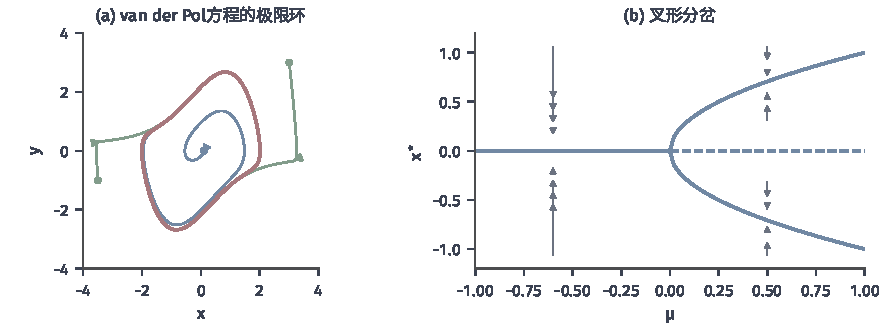
\includegraphics[width=150mm]{figures/03-optimization-evolution-and-signals/02-processes-and-trajectory-evolution/matplotlib/ode-limit-cycle-bifurcation/figure.pdf}
  \caption{平衡点之外的长期行为与参数变化。(a)van der Pol方程$\dot x=y$，$\dot y=(1-x^2)y-x$：从$(0.1,0)$（蓝）以及$(3,3)$、$(-3.5,-1)$（绿）出发的轨迹计算到$t=30$，都趋于红色的极限环。(b)方程$\dot x=\mu x-x^3$的平衡点随参数$\mu$的变化：实线为稳定平衡点，虚线为不稳定平衡点，灰色箭头是$\mu=-0.6$与$\mu=0.5$时状态的运动方向。}
  \label{fig:ode-limit-cycle-bifurcation}
\end{figure*}

\paragraph{参数变化与局部分岔}
向量场含参数时，平衡点及其稳定性会随参数改变。最简单的例子是$\dot x=\mu x-x^3$。$\mu<0$时唯一的平衡点是原点，线性化$\mu<0$，稳定。$\mu>0$时原点的线性化$\mu>0$，变得不稳定，同时出现两个新的平衡点$\pm\sqrt\mu$，其线性化为$\mu-3\mu=-2\mu<0$，都是稳定的。图~\ref{fig:ode-limit-cycle-bifurcation}(b)中平衡点的分支像一把叉子，称为叉形分岔。转变发生在$\mu=0$，那里线性化的特征值穿过零，正是线性化判据失效的临界情形。

van der Pol方程在原点的线性化是$\begin{bmatrix}0&1\\-1&\mu\end{bmatrix}$，特征值$\bigl(\mu\pm\sqrt{\mu^2-4}\bigr)/2$。$\mu$从负变正时，一对复特征值从左向右穿过虚轴，原点由稳定焦点变为不稳定焦点，同时出现极限环。特征值穿过虚轴的位置决定了分岔的类型：穿过零点产生新的平衡点，成对的复特征值穿过虚轴产生周期轨道。完整的分岔理论需要中心流形等工具，本书不展开；这两个低维例子说明，线性化判据的临界情形往往正是定性行为发生改变的地方。

\subsection{持续输入下的轨迹响应}
\label{sec:ode-input-response}

初值误差只在开始时注入一次，稳定系统会逐渐把它忘掉。输入则可以在每个时刻持续地推动状态：暖气的功率一直偏大，房间就一直偏热，不会因为系统“稳定”而回到原来的温度。本小节估计持续输入留下的状态范围，区分哪些部分会被遗忘、哪些部分会保留。

\paragraph{线性系统：初态记忆与输入留下的范围}
设$\bm A$为Hurwitz矩阵，由定理~\ref{thm:ode-linear-spectral-stability}有常数$M\geq1$、$\alpha>0$使$\|e^{t\bm A}\|\leq Me^{-\alpha t}$。对常数变易公式~\eqref{eq:ode-lti-variation}两项分别取范数，得
\begin{equation}
  \|\bm x(t)\|_2\leq Me^{-\alpha(t-t_0)}\|\bm x_0\|_2+M\|\bm B\|\int_{t_0}^te^{-\alpha(t-s)}\|\bm u(s)\|_2\,\mathrm ds.
  \label{eq:ode-linear-input-bound}
\end{equation}
若$\|\bm u(s)\|_2\leq U$，第二项不超过$\frac{M\|\bm B\|U}{\alpha}\bigl(1-e^{-\alpha(t-t_0)}\bigr)$。第一项是初态的记忆，按指数衰减；第二项是输入的累计，最终不超过$M\|\bm B\|U/\alpha$。所以有界输入产生有界状态，状态最终落入半径约为$M\|\bm B\|U/\alpha$的范围，与初态无关。两组初值与输入之差满足同一个线性方程，把上式中的状态、初值和输入分别换成差，就得到两条轨迹的比较界：初值差被遗忘，输入差留下。

以温度模型为例，取示例~\ref{ex:ode-periodic-heating}的周期加热$u(t)=0.4+0.2\sin(0.5t)$。对偏差$x-2$应用式~\eqref{eq:ode-linear-input-bound}，$M=1$、$\alpha=0.2$、$U=0.2$，得
\[
  |x(t)-2|\leq e^{-0.2t}|x_0-2|+\bigl(1-e^{-0.2t}\bigr),
\]
最终范围是$[1,3]$。图~\ref{fig:ode-input-response}显示，从$x_0=0$与$x_0=4$出发的两条轨迹在约$20$分钟后几乎重合，都贴近示例~\ref{ex:ode-periodic-heating}算出的稳态振荡$2+0.371\sin(0.5t-1.19)$。实际振幅$0.371$远小于界给出的$1$：界只用了输入的大小，没有用到输入在快速摆动、正负部分相互抵消这一点。

\begin{figure}[htbp]
  \centering
  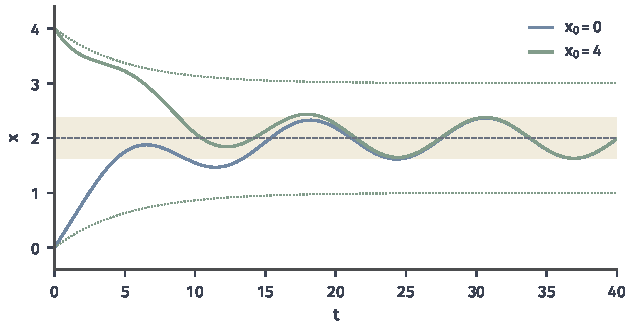
\includegraphics[width=107mm]{figures/03-optimization-evolution-and-signals/02-processes-and-trajectory-evolution/matplotlib/ode-input-response/figure.pdf}
  \caption{持续输入下的温度响应。方程$\dot x=-0.2x+u$，$u(t)=0.4+0.2\sin(0.5t)$。蓝、绿实线分别从$x_0=0$与$x_0=4$出发；同色点线是式~\eqref{eq:ode-linear-input-bound}给出的上下界$2\pm\bigl(e^{-0.2t}|x_0-2|+1-e^{-0.2t}\bigr)$；浅黄带是稳态振荡的范围$2\pm0.371$，灰色虚线为平均平衡值$2$。}
  \label{fig:ode-input-response}
\end{figure}

恒定的偏差最能说明“稳定不消除持续扰动”。若加热量固定偏多$\delta u$，平衡点从$u/\lambda$移到$(u+\delta u)/\lambda$，稳态偏差为$\delta u/\lambda$；$\lambda=0.2$时是$5\,\delta u$。初值的影响以速率$0.2$衰减，这个偏差却一直存在。消除它需要根据测得的温度调整加热量，那是反馈控制的任务。

\paragraph{非线性系统：含输入项的Lyapunov不等式}
非线性系统没有常数变易公式，但Lyapunov函数的方法可以把输入写进下降条件。设$\dot{\bm x}=\bm g(\bm x,\bm u)$，$\bm g(\bm0,\bm0)=\bm0$，并有连续可微的$V$与常数$c_1,c_2,c_3,\gamma>0$，使对一切$\bm x$与输入值$\bm v$，
\begin{equation}
  c_1\|\bm x\|_2^2\leq V(\bm x)\leq c_2\|\bm x\|_2^2,\qquad
  \nabla V(\bm x)^\top\bm g(\bm x,\bm v)\leq-c_3\|\bm x\|_2^2+\gamma\|\bm v\|_2^2.
  \label{eq:ode-iss-lyapunov}
\end{equation}
第二个条件说：状态大时$V$下降，输入大时$V$可以上升，上升的幅度由增益$\gamma$控制。

\begin{theorem}[含输入项的Lyapunov估计]
  \label{thm:ode-iss-bound}
  在条件~\eqref{eq:ode-iss-lyapunov}下，设输入$\bm u$可测且$\|\bm u(t)\|_2\leq U$，$\bm g$关于状态局部Lipschitz并满足Carathéodory条件。则每条解对全部$t\geq t_0$存在，并且
  \[
    \|\bm x(t)\|_2^2\leq\frac{c_2}{c_1}e^{-(c_3/c_2)(t-t_0)}\|\bm x_0\|_2^2+\frac{\gamma c_2}{c_1c_3}U^2.
  \]
\end{theorem}

\begin{proof}
  令$v(t)=V(\bm x(t))$，它沿绝对连续的解几乎处处可导，由条件~\eqref{eq:ode-iss-lyapunov}，$\dot v\leq-c_3\|\bm x\|_2^2+\gamma U^2\leq-(c_3/c_2)v+\gamma U^2$。记$k=c_3/c_2$，则$\frac{\mathrm d}{\mathrm dt}\bigl(e^{k(t-t_0)}v\bigr)\leq\gamma U^2e^{k(t-t_0)}$，积分得$v(t)\leq e^{-k(t-t_0)}v(t_0)+\gamma U^2/k$。再用$c_1\|\bm x\|_2^2\leq v$与$v(t_0)\leq c_2\|\bm x_0\|_2^2$即得所述不等式。它在解的存在区间上成立，说明解留在一个有界集合中，由定理~\ref{thm:ode-escape}，解对全部$t\geq t_0$存在。
\end{proof}

满足这类条件的系统称为\term{输入到状态稳定}（input-to-state stable, ISS）的一种二次形式：初态的影响按指数衰减，输入只留下与其大小成比例的最终范围。例如$\dot x=-x-x^3+u$，取$V=x^2/2$，则$\dot V=-x^2-x^4+xu\leq-x^2+xu\leq-\tfrac12x^2+\tfrac12u^2$，最后一步用了$xu\leq\tfrac12x^2+\tfrac12u^2$。于是$c_1=c_2=c_3=\gamma=\tfrac12$，定理给出$\limsup_{t\to\infty}|x(t)|\leq U$。

无输入时稳定，不等于有输入时有界。$\dot x=-x+x^2u$在$u\equiv0$时原点全局指数稳定；可是取恒定输入$u\equiv1$、$x_0=2$，方程变成$\dot x=x(x-1)$，解为$x(t)=1/(1-e^t/2)$，在$t=\log2$时爆炸。问题在于输入通过$x^2$进入方程，状态越大，输入的作用越强，条件~\eqref{eq:ode-iss-lyapunov}无法成立。本小节分析的是给定系统对给定输入的响应；如何设计依赖状态的输入，使闭环满足这类条件，是反馈稳定化的问题，可参考\BookChapterRef{chap:control-theory}{卷五“策略的实现与轨迹控制”章}。

% 第8章第5节：常微分方程的数值求解（显式Euler与Runge--Kutta；隐式方法与刚性；误差与步长选择）。

\section{常微分方程的数值求解}
\label{sec:ode-numerics}

大多数非线性方程没有闭式解，只能在计算机上一步一步推进。本节固定一个初值问题~\eqref{eq:ode-ivp}与有限时域$[t_0,t_0+T]$，取网格$t_n=t_0+nh$，$n=0,1,\ldots,N$，$Nh=T$，用数值状态$\widehat{\bm x}_n$近似$\bm x(t_n)$。一步数值方法是一个可计算的映射$\widehat{\bm x}_{n+1}=\bm\Psi_h(t_n,\widehat{\bm x}_n)$，它近似精确的演化映射$\bm\varphi_{t_{n+1},t_n}$。我们先构造这类映射，再看刚性怎样改变方法的选择，最后分析误差怎样从每一步累积到终点，以及怎样自动选择步长。

\subsection{显式Euler与Runge--Kutta方法}
\label{sec:ode-euler-rk}

\paragraph{冻结斜率：显式Euler}
最简单的做法是在每一小步内把斜率冻结为起点的值，沿这个方向走$h$时间，再在新位置重新读取斜率：
\begin{equation}
  \widehat{\bm x}_{n+1}=\widehat{\bm x}_n+h\,\bm g(t_n,\widehat{\bm x}_n).
  \label{eq:ode-forward-euler}
\end{equation}
这就是\term{显式Euler法}（explicit Euler method）。在斜率场图上，它相当于沿着当前箭头画一段长为$h$的直线。每步只需调用一次向量场。若向量场在一步之内变化，沿冻结方向走出的直线就会偏离真实的曲线。

衡量偏离的标准是：从精确状态出发走一步，与精确解相差多少。

\begin{definition}[局部截断误差与阶]
  \label{def:ode-local-truncation-error}
  设$\bm x$是精确解。一步方法在$t_n$处的\term{局部截断误差}为
  \[
    \bm\tau_{n+1}=\bm x(t_{n+1})-\bm\Psi_h\bigl(t_n,\bm x(t_n)\bigr).
  \]
  若存在与$n,h$无关的常数$C$，使$\|\bm\tau_{n+1}\|_2\leq Ch^{p+1}$对一切$n$与足够小的$h$成立，称方法的阶为$p$，也称其\term{收敛阶}为$p$。
\end{definition}

局部误差是$h^{p+1}$而阶数记为$p$，是因为走完固定时域需要$N=T/h$步，每步$O(h^{p+1})$的误差累计起来大约是$O(h^p)$；第~\ref{sec:ode-error-step}小节在稳定性条件下证明这一点。对显式Euler，Taylor展开给出$\bm x(t_{n+1})=\bm x(t_n)+h\dot{\bm x}(t_n)+\tfrac{h^2}2\ddot{\bm x}(\xi)$（逐分量取中间点），而$\dot{\bm x}(t_n)=\bm g(t_n,\bm x(t_n))$，所以$\bm\tau_{n+1}=O(h^2)$，阶为$1$。

\paragraph{在一步之内多看几次斜率}
要提高阶数，可以在一步之内多读几次斜率，再把它们组合起来。设$\bm g$足够光滑，沿解有$\ddot{\bm x}=\partial_t\bm g+\partial_{\bm x}\bm g\,\bm g$，于是
\[
  \bm x(t+h)=\bm x+h\bm g+\frac{h^2}2\bigl(\partial_t\bm g+\partial_{\bm x}\bm g\,\bm g\bigr)+O(h^3),
\]
右端各量在$(t,\bm x(t))$处取值。Euler法只匹配了前两项。若先用Euler走半步到中点，再在中点读取斜率，
\[
  \bm k_1=\bm g(t,\bm x),\qquad\bm k_2=\bm g\Bigl(t+\frac h2,\bm x+\frac h2\bm k_1\Bigr)=\bm g+\frac h2\bigl(\partial_t\bm g+\partial_{\bm x}\bm g\,\bm g\bigr)+O(h^2),
\]
那么$\bm x+h\bm k_2$恰好匹配到$h^2$项，局部误差为$O(h^3)$。这就是二阶的中点Runge--Kutta法（下文简称RK2）：
\begin{equation}
  \bm k_1=\bm g(t_n,\widehat{\bm x}_n),\quad
  \bm k_2=\bm g\Bigl(t_n+\frac h2,\widehat{\bm x}_n+\frac h2\bm k_1\Bigr),\quad
  \widehat{\bm x}_{n+1}=\widehat{\bm x}_n+h\bm k_2.
  \label{eq:ode-rk2}
\end{equation}
直观地说，起点的斜率只代表这一步开头的方向，中点的斜率更能代表整一步的平均方向。

沿同样的思路，用四次斜率评估、精心选取的组合系数，可以匹配到$h^4$项，得到经典的四阶Runge--Kutta法（RK4）：
\begin{equation}
  \begin{aligned}
    \bm k_1&=\bm g(t_n,\widehat{\bm x}_n),&
    \bm k_2&=\bm g\Bigl(t_n+\frac h2,\widehat{\bm x}_n+\frac h2\bm k_1\Bigr),\\
    \bm k_3&=\bm g\Bigl(t_n+\frac h2,\widehat{\bm x}_n+\frac h2\bm k_2\Bigr),&
    \bm k_4&=\bm g(t_n+h,\widehat{\bm x}_n+h\bm k_3),\\
    \widehat{\bm x}_{n+1}&=\widehat{\bm x}_n+\frac h6\bigl(\bm k_1+2\bm k_2+2\bm k_3+\bm k_4\bigr).
  \end{aligned}
  \label{eq:ode-rk4}
\end{equation}
若$\bm g$不依赖状态，RK4退化为对$\int_{t_n}^{t_{n+1}}\bm g(s)\,\mathrm ds$的Simpson求积，权重$1,4,1$中的中点权重被分给了$\bm k_2,\bm k_3$。一般地，$s$级显式\term{Runge--Kutta方法}写成
\[
  \bm k_i=\bm g\Bigl(t_n+c_ih,\widehat{\bm x}_n+h\sum_{j<i}a_{i,j}\bm k_j\Bigr),\qquad
  \widehat{\bm x}_{n+1}=\widehat{\bm x}_n+h\sum_{i=1}^sb_i\bm k_i,
\]
系数$a_{i,j},b_i,c_i$由Taylor展开的匹配条件决定，RK4满足四阶的全部条件\scite{math-hairer1993ode}。称$\bm k_i$为阶段变量；每步要调用$s$次向量场，RK2为$2$次，RK4为$4$次。

\paragraph{误差、阶数与计算量}
用一个有解析解的方程检验这些说法。取$\dot x=x\cos t$，$x(0)=1$，分离变量得$x(t)=e^{\sin t}$，终点$x(5)=e^{\sin5}\approx0.3833$。图~\ref{fig:ode-convergence-orders}(a)画出三种方法在$t=5$处的误差随步长的变化。在对数坐标下三条线近似是直线，斜率分别接近$1$、$2$、$4$：步长减半时，Euler的误差减半，RK2的误差变为四分之一，RK4的误差变为约十六分之一（例如$h=0.0098$与$0.0049$时，RK4的误差从$1.42\times10^{-11}$降到$8.9\times10^{-13}$）。

\begin{figure*}[htbp]
  \centering
  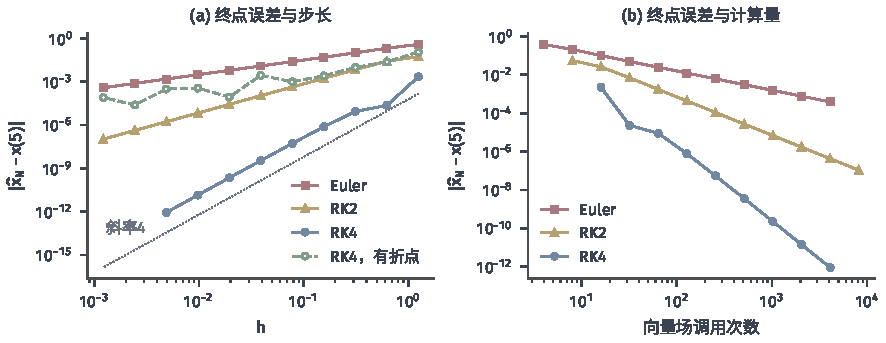
\includegraphics[width=150mm]{figures/03-optimization-evolution-and-signals/02-processes-and-trajectory-evolution/matplotlib/ode-convergence-orders/figure.pdf}
  \caption{终点误差、步长与计算量。方程$\dot x=x\cos t$，$x(0)=1$，比较$t=5$处与$e^{\sin5}$的误差，步长$h=5/2^k$（$k=2,\ldots,12$）。(a)误差对步长，点线为斜率$4$的参考线；绿色空心圆是RK4用于开关加热问题$\dot x=-0.2x+u(t)$（$u$在$t=\pi$处由$0.4$跳到$0$）的误差，跳变时刻不在网格上。(b)同样的误差对向量场调用总次数，Euler、RK2、RK4每步分别调用$1$、$2$、$4$次。}
  \label{fig:ode-convergence-orders}
\end{figure*}

比较效率时，应在同一终止时间、同一误差标准下比较总计算量，而不是比较每步的精度。图~\ref{fig:ode-convergence-orders}(b)把横轴换成向量场调用的总次数。要把误差压到约$10^{-6}$，RK4只需$32$步，即$128$次调用；RK2约需$1333$步，即约$2700$次调用；Euler则需要约$160$万步。高阶方法每步更贵，但能用大得多的步长，在光滑问题上总量反而小得多。

高阶的收益以足够的光滑性为前提。四阶的局部误差估计用到了解的五阶导数；若向量场在时间上有跳变，例如暖气在$t=\pi$时关闭而这个时刻落在某一步内部，RK4的四次斜率读数无法反映跳变发生在步内何处，那一步的局部误差只有$O(h)$量级，仅这一步就使整体误差降为一阶。图~\ref{fig:ode-convergence-orders}(a)中的绿色空心圆正是如此：误差随步长大致按一阶下降，并且随$\pi$在步内的位置而起伏。实际计算中应把已知的跳变时刻放在网格点上，在两侧分段积分。

\subsection{隐式方法与刚性问题}
\label{sec:ode-stiff}

\paragraph{快慢两种尺度}
考虑一个温度传感器：它的读数$x$以很快的速率$k=50$追随环境温度$\cos t$，
\begin{equation}
  \dot x=-k\bigl(x-\cos t\bigr),\qquad x(0)=0,\qquad k=50.
  \label{eq:ode-stiff-example}
\end{equation}
常数变易公式给出精确解$x(t)=\frac{2500\cos t+50\sin t}{2501}-\frac{2500}{2501}e^{-50t}$。最初约$0.1$个时间单位内，$e^{-50t}$项迅速消失；此后解几乎就是缓慢变化的$\cos t$。要准确描绘这条光滑曲线，步长取$0.1$到$0.2$就足够了。

显式Euler却做不到。偏差$e=x-x_{\mathrm{slow}}$近似满足$\dot e=-50e$，Euler把它每步乘以$1-50h$。$h=0.038$时因子为$-0.9$，偏差每步变号并缓慢衰减；$h=0.042$时因子为$-1.1$，偏差每步变号并放大，到$t=3$时数值解已达到约$868$。图~\ref{fig:ode-stiff}(a)画出这两种情形。为了不发散，步长必须小于$2/50=0.04$，这个限制来自早已衰减殆尽的快速分量，而不是来自我们真正想描绘的慢变化。这种“稳定性而非精度限制了显式方法的步长”的现象称为\term{刚性}（stiffness）。

\begin{figure*}[htbp]
  \centering
  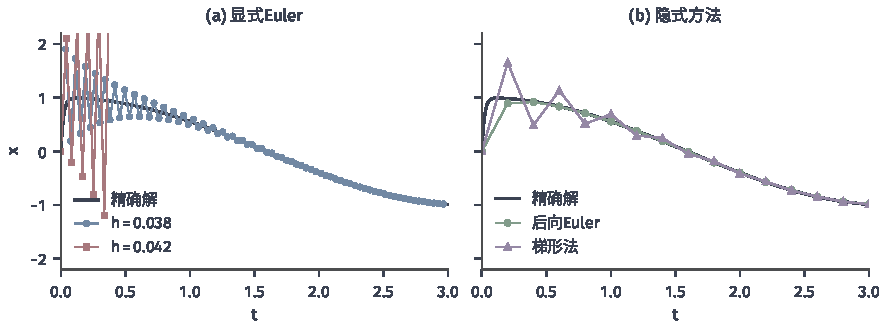
\includegraphics[width=150mm]{figures/03-optimization-evolution-and-signals/02-processes-and-trajectory-evolution/matplotlib/ode-stiff/figure.pdf}
  \caption{刚性方程$\dot x=-50(x-\cos t)$，$x(0)=0$。黑线为精确解。(a)显式Euler：$h=0.038$（蓝）时放大因子为$-0.9$，数值解振荡着缓慢靠近精确解；$h=0.042$（红）时因子为$-1.1$，数值解迅速发散（只画到超出$|x|>3$为止）。(b)步长$h=0.2$的后向Euler（绿）与梯形法（紫）：二者都不发散；后向Euler的放大因子为$1/11\approx0.091$，误差只在开头的快速过渡中可见；梯形法的放大因子为$-2/3$，开头的偏差以交替变号的方式缓慢消退。}
  \label{fig:ode-stiff}
\end{figure*}

\paragraph{线性测试方程与绝对稳定域}
为了把这个现象从具体方程中抽出来，把每个方法用于标量测试方程$\dot x=\lambda x$，$\lambda\in\mathbb C$。线性方程的一步数值映射总是乘以一个只依赖$z=h\lambda$的因子：$\widehat x_{n+1}=R(z)\widehat x_n$。显式Euler的$R(z)=1+z$；RK2与RK4的$R(z)$是$e^z$的Taylor多项式，分别截断到二次与四次：
\[
  R_{\mathrm{RK2}}(z)=1+z+\frac{z^2}2,\qquad R_{\mathrm{RK4}}(z)=1+z+\frac{z^2}2+\frac{z^3}6+\frac{z^4}{24}.
\]

\begin{definition}[绝对稳定域]
  \label{def:ode-absolute-stability}
  一步方法用于测试方程$\dot x=\lambda x$时给出$\widehat x_{n+1}=R(h\lambda)\widehat x_n$。集合$\mathcal S=\{z\in\mathbb C:|R(z)|\leq1\}$称为方法的\term{绝对稳定域}。若$\mathcal S$包含整个闭左半平面$\{\operatorname{Re}z\leq0\}$，称方法\term{A稳定}。
\end{definition}

对线性系统$\dot{\bm x}=\bm A\bm x$，若$\bm A$可对角化，方法在特征坐标下对每个特征值分别作用，数值解不增长的条件是每个$h\lambda_i$都落在$\mathcal S$中。这里要分清两种稳定性：方程的稳定性问的是$\operatorname{Re}\lambda<0$，即精确解是否衰减；方法的稳定性问的是$h\lambda\in\mathcal S$，即数值解是否衰减。前者是方程的性质，后者还依赖步长和方法。

图~\ref{fig:ode-stability-regions}(a)画出三个显式方法的稳定域。Euler的稳定域是以$-1$为心的单位圆盘；RK2稍大，在实轴上同样止于$-2$；RK4更大，在实轴上延伸到约$-2.785$，并且包含虚轴上的一段$|y|\leq2\sqrt2$。刚性例子中$\lambda=-50$，三者的步长上限依次约为$0.04$、$0.04$、$0.056$。显式Runge--Kutta方法的$R$是多项式，$|z|\to\infty$时$|R(z)|\to\infty$，所以稳定域总是有界的，不可能A稳定。提高阶数可以把稳定域扩大一些，却解除不了刚性带来的限制。

\begin{figure*}[htbp]
  \centering
  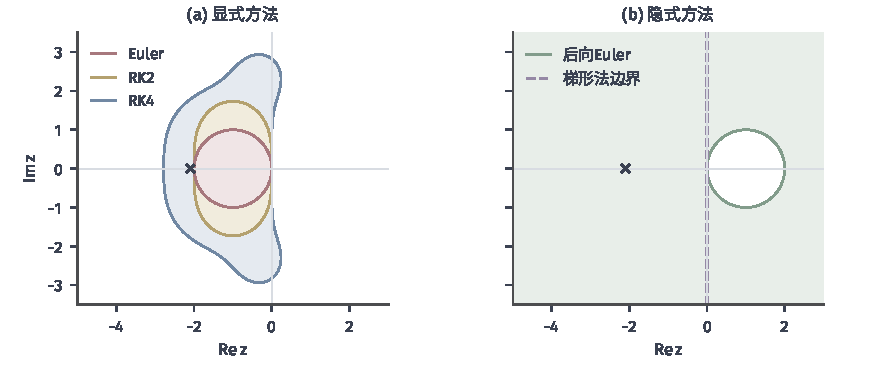
\includegraphics[width=150mm]{figures/03-optimization-evolution-and-signals/02-processes-and-trajectory-evolution/matplotlib/ode-stability-regions/figure.pdf}
  \caption{线性测试方程$\dot x=\lambda x$下的绝对稳定域$\{z=h\lambda:|R(z)|\leq1\}$。(a)显式方法：Euler（红，圆盘）、RK2（黄）、RK4（蓝）；三者在负实轴上分别止于$-2$、$-2$、约$-2.785$。(b)隐式方法：后向Euler的稳定域是以$1$为心的单位圆盘之外的全部区域（绿色填充），梯形法的稳定域恰为闭左半平面（紫色虚线为其边界）。两图中的叉号标出$z=-2.1$。}
  \label{fig:ode-stability-regions}
\end{figure*}

\paragraph{隐式方法}
显式方法只用起点的信息。若改用终点的斜率，
\begin{equation}
  \widehat{\bm x}_{n+1}=\widehat{\bm x}_n+h\,\bm g(t_{n+1},\widehat{\bm x}_{n+1}),
  \label{eq:ode-backward-euler}
\end{equation}
得到\term{后向Euler法}（backward Euler method）。未知的$\widehat{\bm x}_{n+1}$同时出现在两边，每一步都要解一个方程，所以称为隐式方法。用于测试方程，$\widehat x_{n+1}=\widehat x_n+z\widehat x_{n+1}$，即$R(z)=1/(1-z)$；当$\operatorname{Re}z\leq0$时$|1-z|\geq1$，所以后向Euler是A稳定的。它的稳定域甚至包含右半平面的大部分，只排除以$1$为心的单位圆盘。

把起点与终点的斜率平均，得到\term{梯形法}：
\begin{equation}
  \widehat{\bm x}_{n+1}=\widehat{\bm x}_n+\frac h2\Bigl(\bm g(t_n,\widehat{\bm x}_n)+\bm g(t_{n+1},\widehat{\bm x}_{n+1})\Bigr),
  \label{eq:ode-trapezoid}
\end{equation}
其$R(z)=(1+z/2)/(1-z/2)$。$|R(z)|\leq1$恰好等价于$\operatorname{Re}z\leq0$，所以梯形法的稳定域就是闭左半平面：它A稳定，而且是二阶的，后向Euler只有一阶。

A稳定只保证数值解不增长，不保证快速分量被迅速抹去。当$z\to-\infty$时，后向Euler的$R(z)\to0$，快速分量一步就几乎消失；梯形法的$R(z)\to-1$，快速分量几乎不衰减，只是每步变号。对刚性例子取$h=0.2$，$z=-10$，后向Euler的因子为$1/11\approx0.091$，梯形法为$-2/3$；若$h=2$，$z=-100$，梯形法的因子为$-49/51\approx-0.961$，开头的偏差要振荡很久才消退。图~\ref{fig:ode-stiff}(b)显示了$h=0.2$时的差别：后向Euler的误差只在开头的快速过渡中出现，最大约$0.093$；梯形法第一步给出$1.650$，而精确值为$0.984$，此后的偏差交替变号、按$2/3$的比例消退。是否需要强阻尼，取决于是否关心快速过渡阶段本身。

\paragraph{隐式方程怎样求解}
线性方程$\dot{\bm x}=\bm A\bm x+\bm b(t)$的后向Euler步是线性方程组
\[
  (\bm I-h\bm A)\,\widehat{\bm x}_{n+1}=\widehat{\bm x}_n+h\,\bm b(t_{n+1}).
\]
步长固定时，系数矩阵不变，可以只做一次LU分解，以后每步只需回代。刚性例子是标量情形，直接得到$\widehat x_{n+1}=(\widehat x_n+50h\cos t_{n+1})/(1+50h)$。

非线性方程要解$\bm G(\bm y)=\bm y-\widehat{\bm x}_n-h\bm g(t_{n+1},\bm y)=\bm0$。最直接的想法是不动点迭代$\bm y\leftarrow\widehat{\bm x}_n+h\bm g(t_{n+1},\bm y)$，可它是压缩的条件恰是$hL<1$；刚性问题的$L$很大，这个条件与显式方法的步长限制一样苛刻，隐式方法的好处就丢掉了。所以通常用Newton法：从显式Euler给出的预测值出发，反复求解
\[
  \bigl(\bm I-h\,\partial_{\bm x}\bm g(t_{n+1},\bm y^{(k)})\bigr)\bm\delta=-\bm G(\bm y^{(k)}),\qquad\bm y^{(k+1)}=\bm y^{(k)}+\bm\delta.
\]
Newton法在解附近二次收敛，其条件与性质可参考第~\ref{chap:opt-smooth}章。每次迭代需要Jacobian矩阵和一次$d\times d$线性方程组的求解，稠密情形代价为$O(d^3)$；实际中常在若干步之间重用同一个Jacobian及其分解，以牺牲一些收敛速度换取更低的代价。显式方法每步只需若干次向量场调用。因此，隐式方法以更贵的单步换取大得多的稳定步长，只在刚性问题上划算。迭代在有限次后停止，留下的残差相当于每步额外加入的一个小扰动，下一小节把它与截断误差、舍入误差放在一起分析。

后向Euler和梯形法都只用当前一步的信息。线性多步方法还利用前几步的状态，例如二阶后向差分公式
\[
  \frac32\widehat{\bm x}_{n+1}-2\widehat{\bm x}_n+\frac12\widehat{\bm x}_{n-1}=h\,\bm g(t_{n+1},\widehat{\bm x}_{n+1}),
\]
每步只解一个隐式方程就达到二阶，并且A稳定；代价是需要额外的起步值，变步长也更麻烦。A稳定的线性多步方法阶数不超过二，这是多步方法的一个基本限制\scite{math-suli2003numerical}。本书不展开多步方法。

\subsection{局部误差、全局误差与步长选择}
\label{sec:ode-error-step}

\paragraph{误差扇：局部误差怎样累积}
每一步的局部误差都把数值解推到一条邻近的精确解上；此后，精确的动力学会把这条邻近解带向何方，就决定了这个局部误差在终点变成多少。图~\ref{fig:ode-error-fan}把这一过程画出来：从每个数值点出发画一条精确解，红色竖线是每一步的局部误差。

\begin{figure*}[htbp]
  \centering
  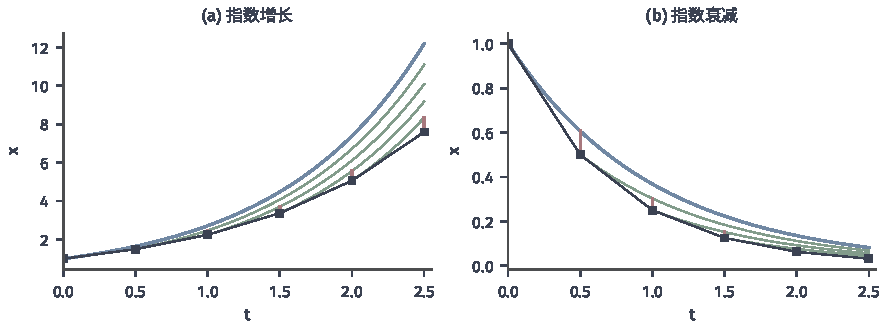
\includegraphics[width=150mm]{figures/03-optimization-evolution-and-signals/02-processes-and-trajectory-evolution/matplotlib/ode-error-fan/figure.pdf}
  \caption{局部误差的传播。显式Euler，步长$h=0.5$，$x(0)=1$，黑色方块为数值解，蓝色是精确解，绿色是从各数值点出发的精确解，红色竖线是每步的局部误差。(a)$\dot x=x$：五个局部误差约为$0.149,0.223,0.335,0.502,0.753$，被增长的流逐步放大，终点误差约为$4.59$。(b)$\dot x=-x$：局部误差约为$0.107,0.053,0.027,0.013,0.007$，被收缩的流逐步抹平，终点误差约为$0.051$。}
  \label{fig:ode-error-fan}
\end{figure*}

两种情形形成鲜明对比。在增长的方程$\dot x=x$中，绿色曲线像扇面一样张开，越早产生的局部误差被放大得越多，终点误差$4.59$远大于局部误差之和$1.96$。在衰减的方程$\dot x=-x$中，绿色曲线相互靠拢，早期的局部误差被逐渐遗忘，终点误差$0.051$小于局部误差之和$0.207$。全局误差由两个因素共同决定：每步产生多少局部误差，以及动力学把它们放大还是缩小。

\paragraph{相容性加稳定性给出收敛}
把这幅图写成不等式。记全局误差$\bm e_n=\widehat{\bm x}_n-\bm x(t_n)$，并允许每步计算带有一个额外扰动$\bm\eta_n$，它可以来自舍入误差，也可以来自隐式方程没有解准的残差：$\widehat{\bm x}_{n+1}=\bm\Psi_h(t_n,\widehat{\bm x}_n)+\bm\eta_n$。于是
\[
  \bm e_{n+1}=\underbrace{\bm\Psi_h(t_n,\widehat{\bm x}_n)-\bm\Psi_h\bigl(t_n,\bm x(t_n)\bigr)}_{\text{已有误差经一步传播}}-\underbrace{\bm\tau_{n+1}}_{\text{局部截断误差}}+\bm\eta_n.
\]
第一项需要数值映射本身不过分放大差别，第二项需要局部误差小。前者称为稳定性，后者称为\term{相容性}（consistency）。下面的离散Grönwall不等式把两者合起来。

\begin{lemma}[离散Grönwall不等式]
  \label{lem:ode-discrete-gronwall}
  设非负数列$\epsilon_n$满足$\epsilon_{n+1}\leq(1+\Lambda h)\epsilon_n+\beta$，其中$\Lambda>0$，$h,\beta\geq0$。则
  \[
    \epsilon_n\leq e^{\Lambda nh}\epsilon_0+\frac{e^{\Lambda nh}-1}{\Lambda h}\,\beta.
  \]
\end{lemma}

\begin{proof}
  归纳展开得$\epsilon_n\leq(1+\Lambda h)^n\epsilon_0+\beta\sum_{j=0}^{n-1}(1+\Lambda h)^j=(1+\Lambda h)^n\epsilon_0+\beta\frac{(1+\Lambda h)^n-1}{\Lambda h}$，再用$1+\Lambda h\leq e^{\Lambda h}$。
\end{proof}

\begin{theorem}[一步方法的有限时域收敛]
  \label{thm:ode-one-step-convergence}
  设精确解$\bm x$在$[t_0,t_0+T]$上存在，$K$是包含精确解与数值解的集合。设
  \begin{enumerate}
    \item （相容性）$\|\bm\tau_{n+1}\|_2\leq Ch^{p+1}$对一切$n$成立；
    \item （稳定性）$\|\bm\Psi_h(t,\bm y)-\bm\Psi_h(t,\bm z)\|_2\leq(1+\Lambda h)\|\bm y-\bm z\|_2$对$\bm y,\bm z\in K$成立，$\Lambda>0$；
    \item （扰动）$\|\bm\eta_n\|_2\leq\eta$对一切$n$成立。
  \end{enumerate}
  则对$nh\leq T$，
  \begin{equation}
    \|\bm e_n\|_2\leq e^{\Lambda T}\|\bm e_0\|_2+\frac{e^{\Lambda T}-1}{\Lambda}\Bigl(Ch^p+\frac\eta h\Bigr).
    \label{eq:ode-global-error}
  \end{equation}
\end{theorem}

\begin{proof}
  由误差递推式及三条假设，$\|\bm e_{n+1}\|_2\leq(1+\Lambda h)\|\bm e_n\|_2+Ch^{p+1}+\eta$。应用引理~\ref{lem:ode-discrete-gronwall}，取$\beta=Ch^{p+1}+\eta$，并用$nh\leq T$。
\end{proof}

式~\eqref{eq:ode-global-error}的三项各有含义。初值误差最多被放大$e^{\Lambda T}$倍，与连续依赖的估计一致。截断误差每步$Ch^{p+1}$，约$T/h$步累计成$O(h^p)$，这就是“局部$h^{p+1}$、全局$h^p$”的来源。每步扰动$\eta$也累计$T/h$次，变成$\eta/h$：步长越小，步数越多，舍入误差积累得越多。所以不断减小步长并不能无限提高精度，存在一个最佳步长，使$Ch^p$与$\eta/h$大致相当。双精度计算的舍入误差约为$10^{-16}$量级，对低阶方法这个下限通常远低于所需精度，对高阶方法和很严的容差则会显现。

对显式Euler，若$\bm g$在$K$上关于状态有Lipschitz常数$L$，则$\|\bm\Psi_h(t,\bm y)-\bm\Psi_h(t,\bm z)\|_2\leq(1+hL)\|\bm y-\bm z\|_2$，稳定性条件对$\Lambda=L$成立；若精确解满足$\|\ddot{\bm x}\|_2\leq M_2$，则$C=M_2/2$。代入式~\eqref{eq:ode-global-error}，从精确初值出发、无额外扰动时得到
\begin{equation}
  \|\widehat{\bm x}_n-\bm x(t_n)\|_2\leq\frac{M_2h}{2L}\bigl(e^{LT}-1\bigr).
  \label{eq:ode-euler-global-error}
\end{equation}
显式Runge--Kutta方法的阶段变量都是$\bm g$的Lipschitz函数，对$h\leq h_0$同样有某个$\Lambda$满足稳定性条件，再配合$p$阶的相容性就得到$O(h^p)$的全局误差。

\paragraph{用方向而不只是大小：单侧Lipschitz条件}
式~\eqref{eq:ode-global-error}中的$e^{\Lambda T}$用的是Lipschitz常数，与第~\ref{sec:ode-continuous-dependence}小节的连续依赖估计有同样的缺点：它只看向量场变化的大小，不看方向。对刚性例子，$L=50$，$e^{50T}$是一个天文数字，估计毫无用处，尽管精确解和后向Euler都在收缩差别。改进的办法是只看差别方向上的分量。若存在$\nu\in\mathbb R$使
\[
  \bigl\langle\bm g(t,\bm y)-\bm g(t,\bm z),\bm y-\bm z\bigr\rangle\leq\nu\|\bm y-\bm z\|_2^2
\]
对一切$\bm y,\bm z$成立，称$\bm g$满足单侧Lipschitz条件，常数$\nu$可以为负。刚性例子中$\nu=-50$，温度模型中$\nu=-\lambda$。

这个条件同时控制精确流和后向Euler。对两条精确解，$\frac{\mathrm d}{\mathrm dt}\frac12\|\bm x-\widetilde{\bm x}\|_2^2\leq\nu\|\bm x-\widetilde{\bm x}\|_2^2$，所以差别按$e^{\nu t}$变化：$\nu<0$时收缩。这正好弥补了第~\ref{sec:ode-continuous-dependence}小节中温度模型的Grönwall上界随时间增长的缺陷。对后向Euler，设两个起点$\bm a,\bm b$分别给出$\bm y,\bm z$，即$\bm y-h\bm g(\bm y)=\bm a$、$\bm z-h\bm g(\bm z)=\bm b$（省略时间变量）。两式相减后与$\bm y-\bm z$作内积，
\[
  \|\bm y-\bm z\|_2^2-h\bigl\langle\bm g(\bm y)-\bm g(\bm z),\bm y-\bm z\bigr\rangle=\langle\bm a-\bm b,\bm y-\bm z\rangle\leq\|\bm a-\bm b\|_2\|\bm y-\bm z\|_2,
\]
左端不小于$(1-h\nu)\|\bm y-\bm z\|_2^2$。所以当$h\nu<1$时，
\[
  \|\bm y-\bm z\|_2\leq\frac{\|\bm a-\bm b\|_2}{1-h\nu}.
\]
$\nu\leq0$时，后向Euler的一步映射对任何步长都不放大差别，稳定性常数与刚性强弱无关。这就是隐式方法在刚性问题上能给出有用误差界的原因。

\paragraph{嵌入式方法估计局部误差}
理论误差界中的常数通常未知，实际计算需要从计算结果本身估计误差，并据此调整步长。最常用的办法是嵌入式方法：用同一组阶段变量构造两个不同阶数的更新，二者之差估计较低阶更新的局部误差。最简单的一对是Heun--Euler对：
\[
  \begin{gathered}
  \bm k_1=\bm g(t_n,\widehat{\bm x}_n),\quad\bm k_2=\bm g(t_n+h,\widehat{\bm x}_n+h\bm k_1),\\
  \bm x^{[1]}=\widehat{\bm x}_n+h\bm k_1,\quad\bm x^{[2]}=\widehat{\bm x}_n+\frac h2(\bm k_1+\bm k_2).
  \end{gathered}
\]
$\bm x^{[1]}$是一阶的Euler步，$\bm x^{[2]}$是二阶的Heun步，二者共用两次向量场调用。由于$\bm x^{[2]}$的局部误差比$\bm x^{[1]}$高一阶，差值$\mathrm{err}=\|\bm x^{[2]}-\bm x^{[1]}\|=\frac h2\|\bm k_2-\bm k_1\|$在主项上等于$\bm x^{[1]}$的局部误差。另一种办法是步长加倍：分别用一步$h$和两步$h/2$推进，比较两个结果。

有了误差估计，步长控制按如下规则进行。给定容差$\mathrm{tol}$：若$\mathrm{err}\leq\mathrm{tol}$，接受这一步，并通常用较高阶的$\bm x^{[2]}$继续（称为局部外推）；否则拒绝，用更小的步长重算这一步。无论接受与否，下一个步长都取
\[
  h_{\mathrm{new}}=h\cdot\min\Bigl\{f_{\max},\ \max\Bigl\{f_{\min},\ 0.9\Bigl(\frac{\mathrm{tol}}{\mathrm{err}}\Bigr)^{1/(q+1)}\Bigr\}\Bigr\},
\]
其中$q$是被估计误差的那个更新的阶（Heun--Euler对中$q=1$）。理由是局部误差约为$Ch^{q+1}$，要让它恰好等于$\mathrm{tol}$，步长应乘以$(\mathrm{tol}/\mathrm{err})^{1/(q+1)}$；因子$0.9$留出安全余量，$f_{\min},f_{\max}$（例如$0.2$与$2$）防止步长剧烈跳动。

\begin{figure}[htbp]
  \centering
  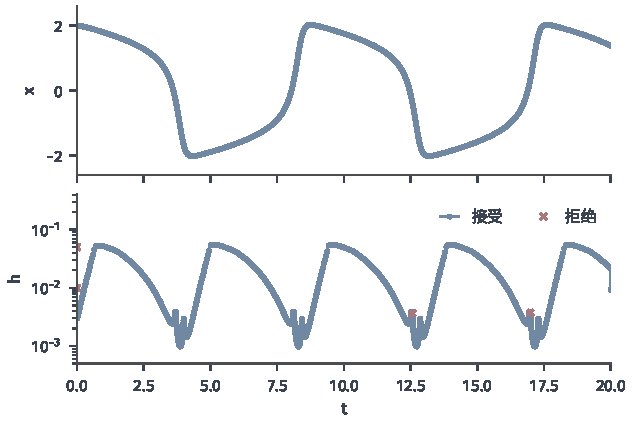
\includegraphics[width=107mm]{figures/03-optimization-evolution-and-signals/02-processes-and-trajectory-evolution/matplotlib/ode-adaptive-step/figure.pdf}
  \caption{自适应步长。van der Pol方程$\dot x=y$，$\dot y=3(1-x^2)y-x$，从$(2,0)$出发计算到$t=20$，使用Heun--Euler对，最大范数容差$10^{-4}$，$f_{\min}=0.2$，$f_{\max}=2$。上图：黑线为参考解的$x$分量，蓝点为接受的数值点。下图：接受的步长（蓝，对数纵轴）与被拒绝的尝试步长（红叉）。}
  \label{fig:ode-adaptive-step}
\end{figure}

图~\ref{fig:ode-adaptive-step}把这个规则用于$\mu=3$的van der Pol方程。解在缓慢漂移与急剧翻转之间交替；步长随之在约$0.056$与$0.00098$之间变化，翻转时自动缩小，漂移时自动放大。全程接受$3221$步、拒绝$4$次，共调用向量场$6450$次；若始终使用最小步长，则需要约$2.0$万步。$t=20$处的实际误差约为$9\times10^{-6}$。

\paragraph{局部误差控制的边界}
自适应方法控制的是每步的局部误差，不是终点的全局误差。误差扇说明，同样的局部误差在增长的动力学下会被放大$e^{\Lambda T}$倍；容差满足了，终点误差仍可能很大，长时间计算或对初值敏感的系统尤其如此。局部误差控制也不保证守恒量或几何结构：对无阻尼的振动系统，每步都合格的误差仍可能沿一个方向持续积累，使能量缓慢漂移，下一节专门处理这个问题。若把显式自适应方法用于刚性问题，步长控制器会发现：步长稍大，快速分量的不稳定就使误差估计变大，于是步长被一再压到稳定极限附近，计算量猛增。这是刚性的一个实用信号，应改用隐式方法。

% 第8章第6节：Hamilton系统与保结构计算（Hamilton方程与守恒结构；辛Euler、Leapfrog与长期误差）。

\section{Hamilton系统与保结构计算}
\label{sec:ode-hamiltonian}

前面的稳定性分析多半依赖耗散：能量或某个Lyapunov函数沿轨迹下降，轨迹最终停下。无摩擦的摆、行星的轨道、分子中原子的振动却不耗散，它们长时间运动而不停下。这类系统的特殊结构既决定了精确解的性质，也对数值方法提出了上一节没有考虑的要求。本节把位置与动量一起作为状态，在欧氏坐标与矩阵形式下研究这种结构；一般流形上的辛几何可参考\BookChapterRef{chap:differential-geometry-and-symmetry}{卷四“非线性空间与流形”章}。

\subsection{Hamilton方程与守恒结构}
\label{sec:ode-hamilton-equations}

\paragraph{从能量写出运动方程}
位置相同而速度不同的物体有不同的未来，所以力学状态要同时记录位置$\bm q\in\mathbb R^d$与动量$\bm p\in\mathbb R^d$。设质量矩阵$\bm M$对称正定，势能$U(\bm q)$连续可微，总能量为动能加势能：
\begin{equation}
  H(\bm q,\bm p)=U(\bm q)+\frac12\bm p^\top\bm M^{-1}\bm p.
  \label{eq:ode-separable-hamiltonian}
\end{equation}
运动方程是：位置的变化率等于速度$\bm M^{-1}\bm p$，动量的变化率等于力$-\nabla U(\bm q)$。对照$H$的偏导数，这恰好是
\begin{equation}
  \dot{\bm q}=\nabla_{\bm p}H,\qquad\dot{\bm p}=-\nabla_{\bm q}H.
  \label{eq:ode-hamilton-equations}
\end{equation}
一个标量函数通过“对动量求导给出位置的变化、对位置求导取负号给出动量的变化”组织出一对方程。摆取$M=1$，$H=p^2/2+1-\cos q$，式~\eqref{eq:ode-hamilton-equations}给出$\dot q=p$、$\dot p=-\sin q$；谐振子取$H=(q^2+p^2)/2$，得$\dot q=p$、$\dot p=-q$。

把$\bm q,\bm p$合成$\bm z=(\bm q^\top,\bm p^\top)^\top\in\mathbb R^{2d}$，方程可以写成一个式子。

\begin{definition}[Hamilton系统]
  \label{def:ode-hamiltonian-system}
  设$H:\mathbb R^{2d}\to\mathbb R$二阶连续可微，令
  \[
    \bm J=\begin{bmatrix}\bm0&\bm I_d\\-\bm I_d&\bm0\end{bmatrix}.
  \]
  方程$\dot{\bm z}=\bm J\nabla H(\bm z)$称为以$H$为\term{Hamilton量}的\term{Hamilton系统}。$H$具有形式~\eqref{eq:ode-separable-hamiltonian}时称为可分的。
\end{definition}

$\bm J$是反对称矩阵，$\bm J^\top=-\bm J$，并且$\bm J^2=-\bm I$。它把梯度转动成运动方向：在$d=1$时，$\bm J\nabla H=(\partial_pH,-\partial_qH)$正是把梯度$(\partial_qH,\partial_pH)$顺时针转了九十度。

\paragraph{同一能量的两种流}
同一个函数$H$可以产生完全不同的动力学。梯度流$\dot{\bm z}=-\nabla H$沿最陡的方向下降；Hamilton流$\dot{\bm z}=\bm J\nabla H$沿与梯度垂直的方向运动。图~\ref{fig:ode-hamilton-gradient-flow}取$H=(q^2+p^2)/2$并从同一点出发：Hamilton流沿圆周永远转下去，梯度流径直落向原点。

\begin{figure}[htbp]
  \centering
  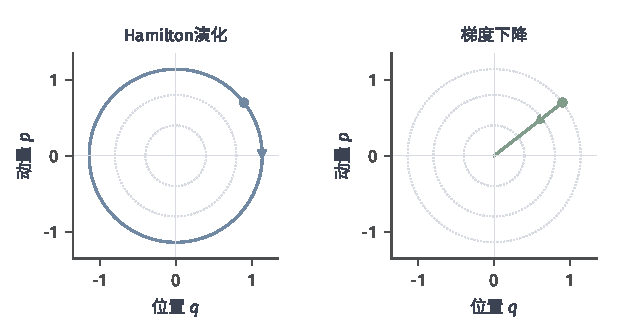
\includegraphics[width=107mm]{figures/00-shared/mathematical-preliminaries-lower/02-dynamical-systems-control-decision-and-games/matplotlib/reader-hamilton-gradient-flow/figure.pdf}
  \caption{同一函数$H(q,p)=(q^2+p^2)/2$下的两种精确流。两面板均从$(q_0,p_0)=(0.9,0.7)$出发，绘制$0\leq t\leq2\pi$；灰色虚线是相同的能量等值线，箭头表示运动方向。左侧Hamilton系统$\dot q=p,\dot p=-q$保持能量，右侧梯度流$\dot q=-q,\dot p=-p$使能量下降。}
  \label{fig:ode-hamilton-gradient-flow}
\end{figure}

两者沿轨迹的能量变化分别是
\[
  \frac{\mathrm d}{\mathrm dt}H=\nabla H^\top\bm J\nabla H=0,\qquad
  \frac{\mathrm d}{\mathrm dt}H=-\nabla H^\top\nabla H=-\|\nabla H\|_2^2,
\]
第一个等式成立是因为反对称矩阵的二次型为零。更一般地，取对称半正定矩阵$\bm R$，方程$\dot{\bm z}=(\bm J-\bm R)\nabla H$满足$\dot H=-\nabla H^\top\bm R\nabla H\leq0$。阻尼摆正是$\bm R=\operatorname{diag}(0,c)$的情形，能量导数为$-cp^2$，这就是第~\ref{sec:ode-lyapunov}小节用过的计算。能量函数相同，动力学由它前面的矩阵决定：反对称部分产生守恒的旋转，对称半正定部分产生耗散。梯度流用于优化，在第~\ref{chap:opt-smooth}章作为离散算法的连续对照出现；Hamilton流则描述保守运动。

\paragraph{能量守恒}
上面对谐振子的计算只用到了$\bm J$的反对称性，并不依赖$H$的具体形式。把它写成一般结论：

\begin{theorem}[Hamilton系统的能量守恒]
  \label{thm:ode-energy-conservation}
  设$H$连续可微，$\bm z(t)$是Hamilton系统在某区间上的解，则$H(\bm z(t))$在该区间上为常数。
\end{theorem}

\begin{proof}
  链式法则给出$\frac{\mathrm d}{\mathrm dt}H(\bm z(t))=\nabla H^\top\dot{\bm z}=\nabla H^\top\bm J\nabla H=0$。
\end{proof}

因此轨迹被限制在初始能量的等值面上。若这些等值面有界（例如势能$U$在无穷远处趋于无穷），轨迹就留在紧集中，由定理~\ref{thm:ode-escape}对全部时间存在。守恒本身并不保证有界：自由粒子$H=p^2/2$保持能量，但$p\neq0$时$q(t)=q_0+pt$无界。若$H$显含时间，同样的计算只给出$\frac{\mathrm d}{\mathrm dt}H=\partial_tH$，能量不再守恒。

\paragraph{辛结构与相空间体积}
能量守恒是对一条轨迹的标量约束，它没有说明一团相邻的初态怎样变形。第~\ref{sec:ode-flows}小节已经看到，无阻尼摆的流把圆盘拉长弯曲，面积却保持不变。现在说明这背后的结构。

取相空间中两个小位移$\bm u,\bm v\in\mathbb R^{2d}$。在$d=1$时，它们张成的平行四边形的有向面积是$u_qv_p-u_pv_q=\bm u^\top\bm J\bm v$。$d>1$时，$\bm u^\top\bm J\bm v=\sum_{i=1}^d(u_{q_i}v_{p_i}-u_{p_i}v_{q_i})$是每一对“位置—动量”坐标平面上有向面积之和。

\begin{definition}[辛形式与辛映射]
  \label{def:ode-symplectic-map}
  对$\bm u,\bm v\in\mathbb R^{2d}$，称$\omega(\bm u,\bm v)=\bm u^\top\bm J\bm v$为标准\term{辛形式}。开集上的连续可微映射$\bm\psi$若在每一点的Jacobian矩阵$\bm G=\partial\bm\psi$都满足
  \begin{equation}
    \bm G^\top\bm J\bm G=\bm J,
    \label{eq:ode-symplectic-condition}
  \end{equation}
  称为\term{辛映射}（symplectic map）。
\end{definition}

条件~\eqref{eq:ode-symplectic-condition}说，任意两个小位移经映射的线性部分作用后，辛形式的值不变。取行列式得$(\det\bm G)^2=1$，所以辛映射保持体积（再由连续性可知行列式为$1$，也保持定向）。反过来不成立：在坐标$(q_1,q_2,p_1,p_2)$下，$\bm G=\operatorname{diag}(2,1,1,\tfrac12)$的行列式为$1$，保持体积，却把第一对坐标平面上的面积乘以$2$、第二对乘以$\tfrac12$，不满足式~\eqref{eq:ode-symplectic-condition}。总体积允许不同坐标对之间相互抵消，辛性不允许。$d=1$时二者等价，辛就是保面积。

\begin{theorem}[Hamilton流是辛映射]
  \label{thm:ode-hamiltonian-flow-symplectic}
  设$H$二阶连续可微，$\bm\varphi_t$是Hamilton系统的流。则在其定义域上，每个$\bm\varphi_t$都是辛映射，并且$\det\partial\bm\varphi_t=1$。
\end{theorem}

\begin{proof}
  由定理~\ref{thm:ode-variational-equation}，$\bm G_t=\partial\bm\varphi_t(\bm z_0)$满足变分方程$\dot{\bm G}_t=\bm J\bm S\bm G_t$，$\bm G_0=\bm I$，其中$\bm S=\nabla^2H(\bm z(t))$是对称的Hessian矩阵。于是
  \[
    \begin{aligned}
    \frac{\mathrm d}{\mathrm dt}\bigl(\bm G_t^\top\bm J\bm G_t\bigr)&=\bm G_t^\top\bigl((\bm J\bm S)^\top\bm J+\bm J\bm J\bm S\bigr)\bm G_t\\
    &=\bm G_t^\top\bigl(\bm S\bm J^\top\bm J+\bm J^2\bm S\bigr)\bm G_t=\bm G_t^\top(\bm S-\bm S)\bm G_t=\bm0,
    \end{aligned}
  \]
  这里用了$\bm J^\top\bm J=\bm I$与$\bm J^2=-\bm I$。初值$\bm G_0^\top\bm J\bm G_0=\bm J$，所以$\bm G_t^\top\bm J\bm G_t=\bm J$。行列式的结论可由定理~\ref{thm:ode-state-transition-properties}的Liouville公式直接得到：$\operatorname{tr}(\bm J\bm S)=\operatorname{tr}(\bm S\bm J^\top)=-\operatorname{tr}(\bm J\bm S)$，故迹为零，$\det\bm G_t=e^0=1$。
\end{proof}

这解释了图~\ref{fig:ode-flow-deformation}：无阻尼摆的流保持面积，阻尼使向量场的迹变为$-c$，面积按$e^{-ct}$缩小。三种性质需要分开：能量守恒是沿一条轨迹的标量性质；体积保持是对一团初值的整体性质；辛性比体积保持更强，约束每一对坐标平面。它们互不蕴含。保持能量而不保持面积的例子是：在谐振子的相平面上用极坐标$(r,\theta)$，令$\bm\psi(r,\theta)=(r,\theta+\epsilon\sin\theta)$，$0<\epsilon<1$。它把每个能量圆映到自身，因而保持$H=r^2/2$；但它沿圆周方向的伸缩率是$1+\epsilon\cos\theta$，不是常数，面积不保持。

\subsection{辛Euler、Leapfrog与长期误差}
\label{sec:ode-symplectic-integrators}

\paragraph{显式Euler为何让能量漂移}
把显式Euler用于谐振子$\dot q=p$，$\dot p=-q$，一步更新为
\[
  \begin{bmatrix}q_{n+1}\\p_{n+1}\end{bmatrix}=\begin{bmatrix}1&h\\-h&1\end{bmatrix}\begin{bmatrix}q_n\\p_n\end{bmatrix},
  \qquad q_{n+1}^2+p_{n+1}^2=(1+h^2)(q_n^2+p_n^2).
\]
每一步能量都精确地乘以$1+h^2$，轨迹沿螺线向外。$h=0.1$时，$120$步后能量变为原来的$1.01^{120}\approx3.30$倍，见图~\ref{fig:ode-symplectic-energy}(a)。后向Euler的因子是$1/(1+h^2)$，轨迹向内螺旋。从稳定域的角度看，谐振子的特征值$\pm\mathrm i$乘以$h$落在虚轴上。显式Euler的稳定域只在原点处碰到虚轴，$|1+\mathrm ih|=\sqrt{1+h^2}>1$；后向Euler在虚轴上（原点除外）满足$|1/(1-\mathrm ih)|<1$。精确流的$|e^{\mathrm ih}|=1$恰好介于二者之间，任何偏向一侧的误差都会在长时间里单调积累。

RK4的稳定域包含虚轴上的一段，在那里$|R_{\mathrm{RK4}}(\mathrm iy)|^2=1-y^6/72+y^8/576$，对$0<|y|\leq2\sqrt2$略小于$1$。所以RK4用于谐振子时能量也单调地减小，只是每步的损失是$O(h^6)$，很慢。问题不在于阶数不够高，而在于方法没有尊重系统的结构。

\paragraph{辛Euler与Leapfrog}
对可分的Hamilton量，可以把一步拆成两种可以精确求解的子运动。只保留势能时，$\dot{\bm q}=\bm0$，$\dot{\bm p}=-\nabla U(\bm q)$，位置不动，动量受一次“冲击”：$(\bm q,\bm p)\mapsto(\bm q,\bm p-c\nabla U(\bm q))$，记为$\bm\Phi_U^c$。只保留动能时，$\dot{\bm q}=\bm M^{-1}\bm p$，$\dot{\bm p}=\bm0$，动量不变，位置“漂移”：$(\bm q,\bm p)\mapsto(\bm q+c\bm M^{-1}\bm p,\bm p)$，记为$\bm\Phi_K^c$。两者都是对应子系统的精确流。

先冲击、再漂移，得到\term{辛Euler法}：
\begin{equation}
  \bm p_{n+1}=\bm p_n-h\nabla U(\bm q_n),\qquad\bm q_{n+1}=\bm q_n+h\bm M^{-1}\bm p_{n+1}.
  \label{eq:ode-symplectic-euler}
\end{equation}
与显式Euler的唯一区别是：位置更新使用已经更新过的动量。把冲击对半分开、夹住一次整步漂移，得到对称的\term{Leapfrog方法}（也称蛙跳法或Störmer--Verlet方法）：
\begin{equation}
  \begin{aligned}
  \bm p_{n+1/2}&=\bm p_n-\frac h2\nabla U(\bm q_n),\\
  \bm q_{n+1}&=\bm q_n+h\bm M^{-1}\bm p_{n+1/2},\\
  \bm p_{n+1}&=\bm p_{n+1/2}-\frac h2\nabla U(\bm q_{n+1}).
  \end{aligned}
  \label{eq:ode-leapfrog}
\end{equation}
即$\bm\Psi_h=\bm\Phi_U^{h/2}\circ\bm\Phi_K^h\circ\bm\Phi_U^{h/2}$。连续两步之间，后一步开头的半步冲击与前一步结尾的半步冲击使用同一个力$\nabla U(\bm q_{n+1})$，所以每步只需计算一次力。辛Euler是一阶方法，Leapfrog是二阶方法。

用于谐振子（$U=q^2/2$，$M=1$），两者的更新矩阵分别是
\[
  \begin{bmatrix}1-h^2&h\\-h&1\end{bmatrix},\qquad
  \begin{bmatrix}1-h^2/2&h\\-h+h^3/4&1-h^2/2\end{bmatrix},
\]
行列式都是$1$。图~\ref{fig:ode-symplectic-energy}(a)中，两者在$120$步内都紧贴单位圆，没有向外或向内的漂移。

\begin{figure*}[htbp]
  \centering
  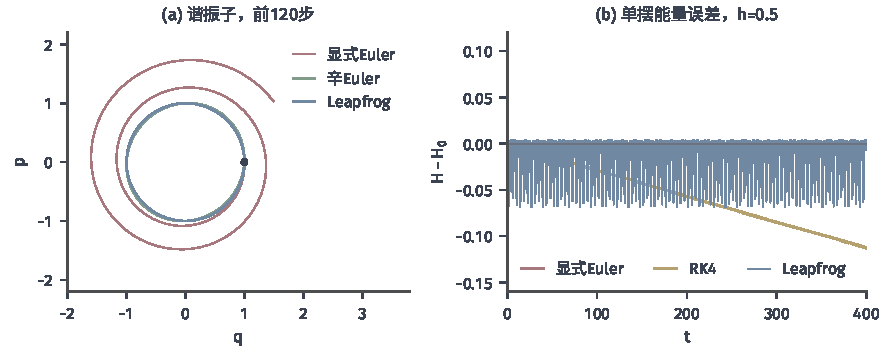
\includegraphics[width=150mm]{figures/03-optimization-evolution-and-signals/02-processes-and-trajectory-evolution/matplotlib/ode-symplectic-energy/figure.pdf}
  \caption{保守系统的长期数值行为。(a)谐振子$\dot q=p$，$\dot p=-q$，从$(1,0)$出发，步长$h=0.1$，各算$120$步：显式Euler（红）的能量按$1.01^n$增长，$120$步后为初值的约$3.30$倍；辛Euler（绿）与Leapfrog（蓝）贴近灰色虚线所示的精确圆周。(b)单摆$\dot q=p$，$\dot p=-\sin q$，从$(2,0)$出发（$H_0=1-\cos2\approx1.416$），步长$h=0.5$，计算到$t=400$，纵轴为能量误差$H-H_0$：显式Euler在约$t=3$时误差即超出图示范围；RK4（黄）单调下降到约$-0.113$；Leapfrog（蓝）在$[-0.069,0.004]$内振荡而不漂移。}
  \label{fig:ode-symplectic-energy}
\end{figure*}

\paragraph{验证保辛与可逆}
设$U$二阶连续可微。冲击与漂移的Jacobian矩阵为
\[
  \bm G_U=\begin{bmatrix}\bm I&\bm0\\-c\nabla^2U&\bm I\end{bmatrix},\qquad
  \bm G_K=\begin{bmatrix}\bm I&c\bm M^{-1}\\\bm0&\bm I\end{bmatrix}.
\]
直接相乘可验证$\bm G_U^\top\bm J\bm G_U=\bm J$：计算中出现的是$-c\nabla^2U+c(\nabla^2U)^\top$，由Hessian矩阵的对称性为零；同理$\bm M^{-1}$的对称性给出$\bm G_K^\top\bm J\bm G_K=\bm J$。辛映射的复合仍是辛映射，因为$(\bm G_1\bm G_2)^\top\bm J(\bm G_1\bm G_2)=\bm G_2^\top(\bm G_1^\top\bm J\bm G_1)\bm G_2=\bm G_2^\top\bm J\bm G_2=\bm J$。所以辛Euler与Leapfrog都是辛映射。这也说明了它们为何与显式Euler不同：显式Euler同时用旧的位置和旧的动量更新两者，用于谐振子时Jacobian的行列式是$1+h^2$，不是辛映射。

Leapfrog还有一个对称性。每个子步把$c$换成$-c$就得到它的逆，而三个子步对称排列，所以$\bm\Psi_h^{-1}=\bm\Psi_{-h}$：向后走一步等于把步长取负。若$\bm R(\bm q,\bm p)=(\bm q,-\bm p)$表示动量反向，还有$\bm R\circ\bm\Psi_h\circ\bm R=\bm\Psi_h^{-1}$：把动量反过来走一步，再把动量反回来，恰好回到出发前的状态。这就是数值上的时间可逆性，与精确流的可逆性相对应。辛Euler没有这种对称性，它的逆是“先漂移、后冲击”的另一种排列。

\paragraph{保辛不等于精确保能量}
辛方法并不精确保持$H$。对谐振子的Leapfrog，更新矩阵的迹为$2-h^2$，行列式为$1$；当$0<h<2$时，两个特征值是单位圆上一对不同的共轭复数，可以直接验证它精确保持修正的二次型
\[
  \widetilde H_h(q,p)=\Bigl(1-\frac{h^2}4\Bigr)q^2+p^2.
\]
这是一族椭圆而不是原来的能量圆。例如从$(1,0)$出发取$h=1$，一步得到$(\tfrac12,-\tfrac34)$，原能量从$\tfrac12$变成$\tfrac{13}{32}$，修正二次型却保持为$\tfrac34$。原能量在椭圆上周期性地变化，偏差是$O(h^2)$，但不会单调地漂移。辛Euler类似地保持$q^2+p^2-hqp$。$h>2$时Leapfrog的更新矩阵有模大于$1$的特征值，数值解指数增长；保辛并不意味着任意步长都稳定。

非线性情形没有这样简单的修正二次型。图~\ref{fig:ode-symplectic-energy}(b)取单摆与较大的步长$h=0.5$计算到$t=400$：Leapfrog的能量误差始终在$[-0.069,0.004]$内振荡；RK4每步的局部误差小得多，能量却单调下降，到$t=400$约少了$0.113$；显式Euler的能量误差在$t\approx3$时就超出了图示范围。还要注意，RK4每步调用$4$次向量场，Leapfrog只需$1$次力的计算。对一般光滑的Hamilton量，辛方法在长时间内能量误差有界的表现，依赖步长足够小、$H$足够光滑以及轨道留在有界区域等条件，相应的理论（后向误差分析）超出本书范围。

\paragraph{用于采样时还缺什么}
Leapfrog的保体积与可逆性，使它成为Hamilton Monte Carlo采样中的标准积分器\scite{pgm-sampling-neal2011}。但它不能单独完成采样。精确的Hamilton流保持能量，只在一个能量等值面上运动，无法探索不同能量的状态，所以需要定期从相应分布中重新抽取动量。Leapfrog又只近似保持能量，若不加修正，所得样本的分布会有偏差，所以每条数值轨迹的终点还要按能量误差决定是否接受。保辛、可逆和保体积使这个接受概率可以简单地计算，但并不能代替它。完整的构造与正确性证明属于随机过程，在第~\ref{chap:discrete-time-stochastic-processes}章讨论。

% 第8章第7节：本章小结。

\section{本章小结}
\label{sec:ode-summary}

本章从“只知道每个瞬间的变化率，能否确定整条轨迹”出发。第~\ref{sec:ode-ivp}节把问题写成初值问题：向量场规定瞬时方向，积分方程把方向累计成状态；输入只在时间上可测时，解放宽为几乎处处满足方程的绝对连续曲线，而不是任意连续曲线。第~\ref{sec:ode-well-posedness}节用同一个积分方程回答了章首的第一组问题：在关于状态局部Lipschitz的条件下，积分映射在短时间的曲线空间里是压缩映射，解局部存在且唯一；局部解按唯一性拼接成最大解，它在有限时间内停止的唯一方式是离开状态集合中的每个紧集，线性增长条件借助Grönwall不等式排除了这种情形；初值、输入与模型的误差在有限时间内至多按$e^{Lt}$放大，可微时由变分方程给出一阶灵敏度。只有连续性时解可能不唯一，增长过快时解可能在有限时间爆炸，这两个反例标出了条件的边界。

第~\ref{sec:ode-analytic-solutions}节在可以求解的方程上落实这些结论。可分离变量方程把时间写成路程除以速度的积分，统一解释了爆炸与有限时间离开平衡点；常数变易公式把解分成初值的记忆与输入的累计；矩阵指数与状态转移矩阵给出线性系统的完整解法，其中时变系数的传播必须保留时间次序。零阶保持离散化在输入分段常值时是精确的，这一点把连续模型与离散模型准确地联系起来。

第~\ref{sec:ode-stability}节回答长期行为。线性系统的稳定性由特征值相对虚轴的位置决定，但非正规矩阵可能在衰减之前先放大；Lyapunov方程为稳定的线性系统提供一个单调下降的二次度量，线性化把这一结论推广到非线性平衡点的邻域。要对更大的区域下结论，需要Lyapunov函数；能量只是非严格下降时，LaSalle不变性原理用$\omega$极限集的不变性排除那些不能持续停留的零导数点。梯度流说明下降有下界并不等于状态收敛，极限环与分岔说明长期行为不只是趋于平衡点。持续输入下，稳定系统会遗忘初态，却会把输入的大小留在状态的最终范围中。

第~\ref{sec:ode-numerics}节与第~\ref{sec:ode-hamiltonian}节回答计算问题。一步方法的全局误差由相容性与稳定性共同控制：局部截断误差$O(h^{p+1})$经约$T/h$步累计为$O(h^p)$，舍入与隐式方程的残差则随步数增加而积累。刚性问题中，显式方法的步长受稳定域而非精度限制，A稳定的隐式方法以每步求解方程为代价解除这一限制，单侧Lipschitz条件说明了它们的误差界为何不随刚性恶化。自适应步长控制局部误差，却不能保证全局误差或长期的结构性质。对保守系统，精确流保持能量、辛结构与相空间体积，三者互不蕴含；辛Euler与Leapfrog保持辛结构而只近似保持能量，在合适的步长下能量误差有界而不漂移，这是阶数更高的通用方法做不到的。

两个贯穿例子概括了向量场结构的作用。温度模型和阻尼摆是耗散的：误差与初值记忆随时间消退，长期行为由稳定性理论刻画，数值方法要关心的是稳定域与刚性。无阻尼摆是保守的：误差不会自动消退，长期行为是在能量面上的永恒运动，数值方法要关心的是能否尊重这种结构。区分这些结论时，还要注意每一条结论作用于真实轨迹还是离散近似，以及它在有限时间内还是在长期成立。

本章的状态是有限维向量。若未知量是一根杆上的温度分布或一张膜的位移，状态就成为空间区域上的函数，方程中出现对空间变量的导数，边界上的条件也成为问题的一部分。第~\ref{chap:partial-differential-equations}章研究这种情形，本章的时间推进方法将在那里作为空间离散之后的求解工具再次出现。

